\documentclass{article}
\usepackage{xeCJK}
\usepackage[T1]{fontenc}
\setCJKmainfont[BoldFont=FandolSong-Bold,ItalicFont=FandolKai-Regular]{FandolSong-Regular}
\setCJKsansfont[BoldFont=FandolHei-Bold]{FandolHei-Regular}
\setCJKmonofont{FandolFang-Regular}
\usepackage[preprint]{colm2025_conference} 
\usepackage{xcolor}
\usepackage{hyperref}
\usepackage[margin=1.25in]{geometry}
\usepackage{graphicx}
\usepackage{amsmath}
\usepackage{amsfonts}
\usepackage{amssymb}
\usepackage{booktabs}
\usepackage{adjustbox}
\usepackage{cellspace}
\usepackage{wrapfig}
\usepackage{amsthm}
\usepackage[ruled,linesnumbered,noresetcount]{algorithm2e}
\usepackage{mathtools}
\usepackage{csquotes}
\usepackage{array}
\usepackage{url,eucal}
\usepackage{tabularx}
\usepackage{makecell}
\newtheorem{theorem}{定理}
\theoremstyle{definition}
\newtheorem{definition}{定义}[section]
\newtheorem{proposition}{命题}
\newtheorem*{explanation}{说明}
\DeclareMathOperator*{\argmax}{arg\,max}
\DeclareMathOperator*{\argmin}{arg\,min}
\DeclareMathOperator\supp{supp}
\DeclareMathOperator\image{Im}

\setlength{\marginparwidth}{0.8in}

\title{世界模型的定义与发展路线图}



\author{上海人工智能实验室物理智能团队}



% Translate labels while retaining the original style definitions.
\renewcommand{\contentsname}{目录}
\renewcommand{\figurename}{图}
\renewcommand{\tablename}{表}
\renewcommand{\refname}{参考文献}
\usepackage{etoolbox}
\patchcmd{\abstract}{Abstract}{摘要}{}{\PackageError{translation}{Abstract label not found}{}}
\hypersetup{hidelinks,unicode=true,pdftitle={世界模型的定义与发展路线图},pdfauthor={上海人工智能实验室物理智能团队}}
% Chinese typesetting on top of the original COLM article template.
% Keep the original paper, text area, numbering, figures and page furniture.
\usepackage{indentfirst}
\usepackage{xurl}
\usepackage{caption}
\usepackage{needspace}
\captionsetup{font=small,labelfont=bf,skip=7pt}

\makeatletter
\renewcommand{\normalsize}{%
  \@setfontsize\normalsize{11pt}{17.6pt}%
  \abovedisplayskip 9pt plus 2pt minus 2pt
  \belowdisplayskip 9pt plus 2pt minus 2pt
  \abovedisplayshortskip 3pt plus 2pt
  \belowdisplayshortskip 6pt plus 2pt minus 2pt}
\renewcommand{\small}{\@setfontsize\small{10pt}{15pt}}
\renewcommand{\footnotesize}{\@setfontsize\footnotesize{9pt}{13.5pt}}
\renewcommand{\scriptsize}{\@setfontsize\scriptsize{7.5pt}{10pt}}
\renewcommand{\tiny}{\@setfontsize\tiny{6.5pt}{8pt}}
\renewcommand{\large}{\@setfontsize\large{13pt}{20pt}}
\renewcommand{\Large}{\@setfontsize\Large{16pt}{24pt}}
\renewcommand{\LARGE}{\@setfontsize\LARGE{18pt}{27pt}}
\renewcommand{\huge}{\@setfontsize\huge{20pt}{30pt}}
\renewcommand{\Huge}{\@setfontsize\Huge{24pt}{34pt}}

\renewcommand{\section}{\@startsection{section}{1}{\z@}%
  {18pt plus 2pt minus 2pt}{8pt plus 1pt}%
  {\large\sffamily\bfseries\raggedright}}
\renewcommand{\subsection}{\@startsection{subsection}{2}{\z@}%
  {13pt plus 2pt minus 1pt}{5pt plus 1pt}%
  {\fontsize{12pt}{19pt}\selectfont\sffamily\bfseries\raggedright}}
\renewcommand{\subsubsection}{\@startsection{subsubsection}{3}{\z@}%
  {10pt plus 1pt minus 1pt}{4pt plus 1pt}%
  {\normalsize\sffamily\bfseries\raggedright}}
\patchcmd{\@maketitle}{\Large\bf}%
  {\fontsize{18pt}{26pt}\selectfont\sffamily\bfseries}{}%
  {\PackageError{translation}{Title font patch failed}{}}
\patchcmd{\@maketitle}{\hsize\textwidth}%
  {\hsize\textwidth\parindent=0pt}{}%
  {\PackageError{translation}{Title indentation patch failed}{}}
\patchcmd{\abstract}{\large\bf}{\large\sffamily\bfseries}{}%
  {\PackageError{translation}{Abstract font patch failed}{}}
\pretocmd{\l@section}{\Needspace{3\baselineskip}}{}%
  {\PackageError{translation}{Contents spacing patch failed}{}}

% Keep numbered-heading link targets inside the heading line. Otherwise a
% preceding float page can capture the vertical-mode target in XeLaTeX.
\newcommand{\zh@headingstep}[1]{%
  \let\zh@savedraisedlink\Hy@raisedlink
  \def\Hy@raisedlink##1{\def\zh@headinganchor{\Hy@raisedlink{##1}}}%
  \refstepcounter{#1}%
  \let\Hy@raisedlink\zh@savedraisedlink}
\pretocmd{\NR@sect}{\let\zh@headinganchor\@empty}{}%
  {\PackageError{translation}{Heading target initialization failed}{}}
\patchcmd{\NR@sect}{\refstepcounter}{\zh@headingstep}{}%
  {\PackageError{translation}{Heading counter patch failed}{}}
\patchcmd{\NR@sect}{\@hangfrom{\hskip #3\relax\@svsec}}%
  {\@hangfrom{\hskip #3\relax\zh@headinganchor\@svsec}}{}%
  {\PackageError{translation}{Heading target placement failed}{}}

\renewcommand{\@listi}{%
  \leftmargin\leftmargini
  \topsep 5pt plus 1pt minus 1pt
  \partopsep 0pt
  \itemsep 3pt plus 1pt minus 1pt
  \parsep 2pt plus 1pt minus 1pt}
\makeatother

\normalsize
\setlength{\parindent}{2em}
\setlength{\parskip}{3pt plus 1pt minus 1pt}
\setlength{\footnotesep}{9pt}
\setlength{\skip\footins}{12pt plus 2pt minus 2pt}
\setlength{\headheight}{16pt}
\addtolength{\topmargin}{-4pt}
\renewcommand{\bibfont}{\fontsize{9.5pt}{12.5pt}\selectfont}
\setlength{\bibsep}{4pt plus 1pt minus 1pt}
% Larger Chinese headings and leading need room below top-of-page figures.
\renewcommand{\textfraction}{0.12}
\raggedbottom

\begin{document}
\maketitle


\begin{abstract}
世界模型（World Model）是学习环境结构与动力学的内部模拟器，已成为人工智能领域讨论最活跃的概念之一。从基于模型的强化学习（model-based reinforcement learning，MBRL）、视频生成，到具身机器人乃至物理人工智能（Physical AI），各个子领域的研究者都在构建被称为“世界模型”的系统。然而，对于世界模型究竟是什么、应当预测什么、应当如何构建，目前尚无共识。本文作为一篇观点文章，给出世界模型的科学定义，讨论其关键技术问题，并提出构建有效世界模型的分阶段发展路线图。
\end{abstract}

\tableofcontents
\clearpage


\section{引言}

“世界模型”一词在不同语境中积累了多种用法，既揭示了一些含义，也掩盖了另一些含义。早在1943年，\cite{craik1943nature}便提出，生物体通过在头脑中维持物理世界的“工作模型”（working model）来生存和繁衍。这些模型使心智能够模拟假想情境、预测候选行动的结果，并预先计算最优策略，而不必完全依赖缓慢的物理试错交互。这一思想的算法实现，正是今天所谓“世界行动模型”（World Action Model，WAM）的形式化体现。Craik的假说为强化学习智能体和生成模型等重要人工智能架构奠定了思想基础\citep{sutton2018rl}。计算机视觉、机器人学和生成建模等领域都使用这一概念，但它们所指的系统往往大不相同。近年来，最有影响的概念澄清尝试是李飞飞（Fei-Fei Li）提出的功能分类：将世界模型划分为\textit{渲染器（renderer）}（生成像素）、\textit{模拟器（simulator）}（预测状态转移）和\textit{规划器（planner）}（提出行动）三类\citep{worldlabs2026taxonomy}。

这一功能分类有助于澄清概念，但它的根本局限在于：所划分的是表征（representation）的\textit{解码方式（decoding）}（也称投影），而非表征本身。一个统一的内部模型可以根据调用的查询接口，解码为RGB像素、状态向量或候选行动方案。该分类规定了世界模型输出什么，却没有定义内部模型是什么、应当如何构建。上游问题——如何构建一种共享的内部表征，以支持这三种解码——仍是功能分类尚未回答的问题。

另一种观点以\cite{lecun2022path}的论述最具代表性，认为生成式重建从来都不是正确的目标：在潜在空间（latent space）中进行预测的联合嵌入架构（joint-embedding architecture）已经足够，而像素级重建会将表征容量浪费在无关的光度细节上。我们赞同，精确的像素级重建不应成为世界模型的终极目标；不过，重建质量有助于查明压缩表征没有保留哪些信息。最终，重建对世界建模究竟有多重要，只能通过测试来判断。

关于压缩表征，如今人们普遍认为，大语言模型（large language model，LLM）擅长压缩人类的\textit{语言}知识。类似地，世界模型是一种统一的压缩机制（compression mechanism），其核心目标是尽可能压缩\textit{现实世界物理感官观测与智能体行动的联合分布}。有损压缩带来了不可避免的表征取舍，形成一条连续谱：潜在表征可以偏向紧凑的高层语义抽象，也可以优先保留细粒度物理动力学和感知保真度；所有实际世界模型都在这两个极端之间取得某种平衡。这种以压缩为中心的观点，或许更能刻画当前研究中的架构选择、数据约束和经验瓶颈。

\paragraph{数据决定能力上限}
我们的出发点是一个简单却影响深远的前提：任何智能系统在物理世界中的泛化能力上限，都由训练数据所包含的物理经验多样性决定。在架构和计算预算固定的条件下，决定这一上限的是数据多样性，而非模型结构或训练超参数。架构与计算量影响系统接近上限的效率，却不能抬高上限\citep{hoffmann2022training}。

目前，唯一能够扩展到所需多样性的物理数据来源，是开放互联网中数以千亿计的图像、视频和文本样本。专有数据来源——灵巧操作数据集、第一人称具身记录以及安装在外骨骼上的传感器——在多样性和规模上都受到结构性限制。在可预见的未来，无论部署多少硬件，都无法产生互联网规模的操作数据。因此，要构建能够泛化到物理世界的“世界模型”，就必须从现有数据中尽可能多地提取物理理解。

尤其是互联网视频，它是规模空前的自然语料库，以完全隐含的方式编码了极其广泛、具有结构的物理世界知识。日常视频的原始像素流中，蕴藏着支配物理现实的基本先验：物体恒存性（object permanence，即物体在视野之外仍持续存在）、区分刚体与可变形材料的刚性和非刚性约束、物体运动与交互的运动学限制、光照和阴影的时间变化、遮挡与显露的因果逻辑、事件的层级因果链，以及类人行动与交互的结构先验。\textit{关键困难在于，所有这些物理结构在原始像素空间中都处于潜在状态，无法直接获取。}

图\ref{fig:data1}给出了我们提出的\textbf{倒金字塔工作流（Inverted Pyramid Workflow）}，用以解决上述核心困难。原始互联网视频中蕴藏着潜在物理先验，但这些先验埋藏在无标签像素中；专有机器人硬件又无法独立产生规模和多样性相当的数据。该流程以互联网中范围极广的真实物理场景影像为基础，首先通过自动筛选和标注，释放其中潜在、隐含的物理知识，以数据多样性提高世界模型的泛化上限。随后逐级收窄的数据漏斗起到精细蒸馏的作用：去除无关视觉内容，合成标准化行动表征，只保留机器人所需、具有物理意义的运动与交互信号。最终形成规模紧凑、符合任务要求的真实世界数据集，使模型能够在具身操作任务上高效收敛，同时保留从数十亿互联网视频中提取的广泛物理先验。架构与计算量只决定模型学习的速度；这一倒置流程则扩展了训练语料中基础物理经验的多样性，提高了世界模型对未见现实物体、运动和因果情境的泛化上限，而这些内容无法被规模有限的专有机器人数据集充分涵盖。

\begin{figure}[h]
    \centering
    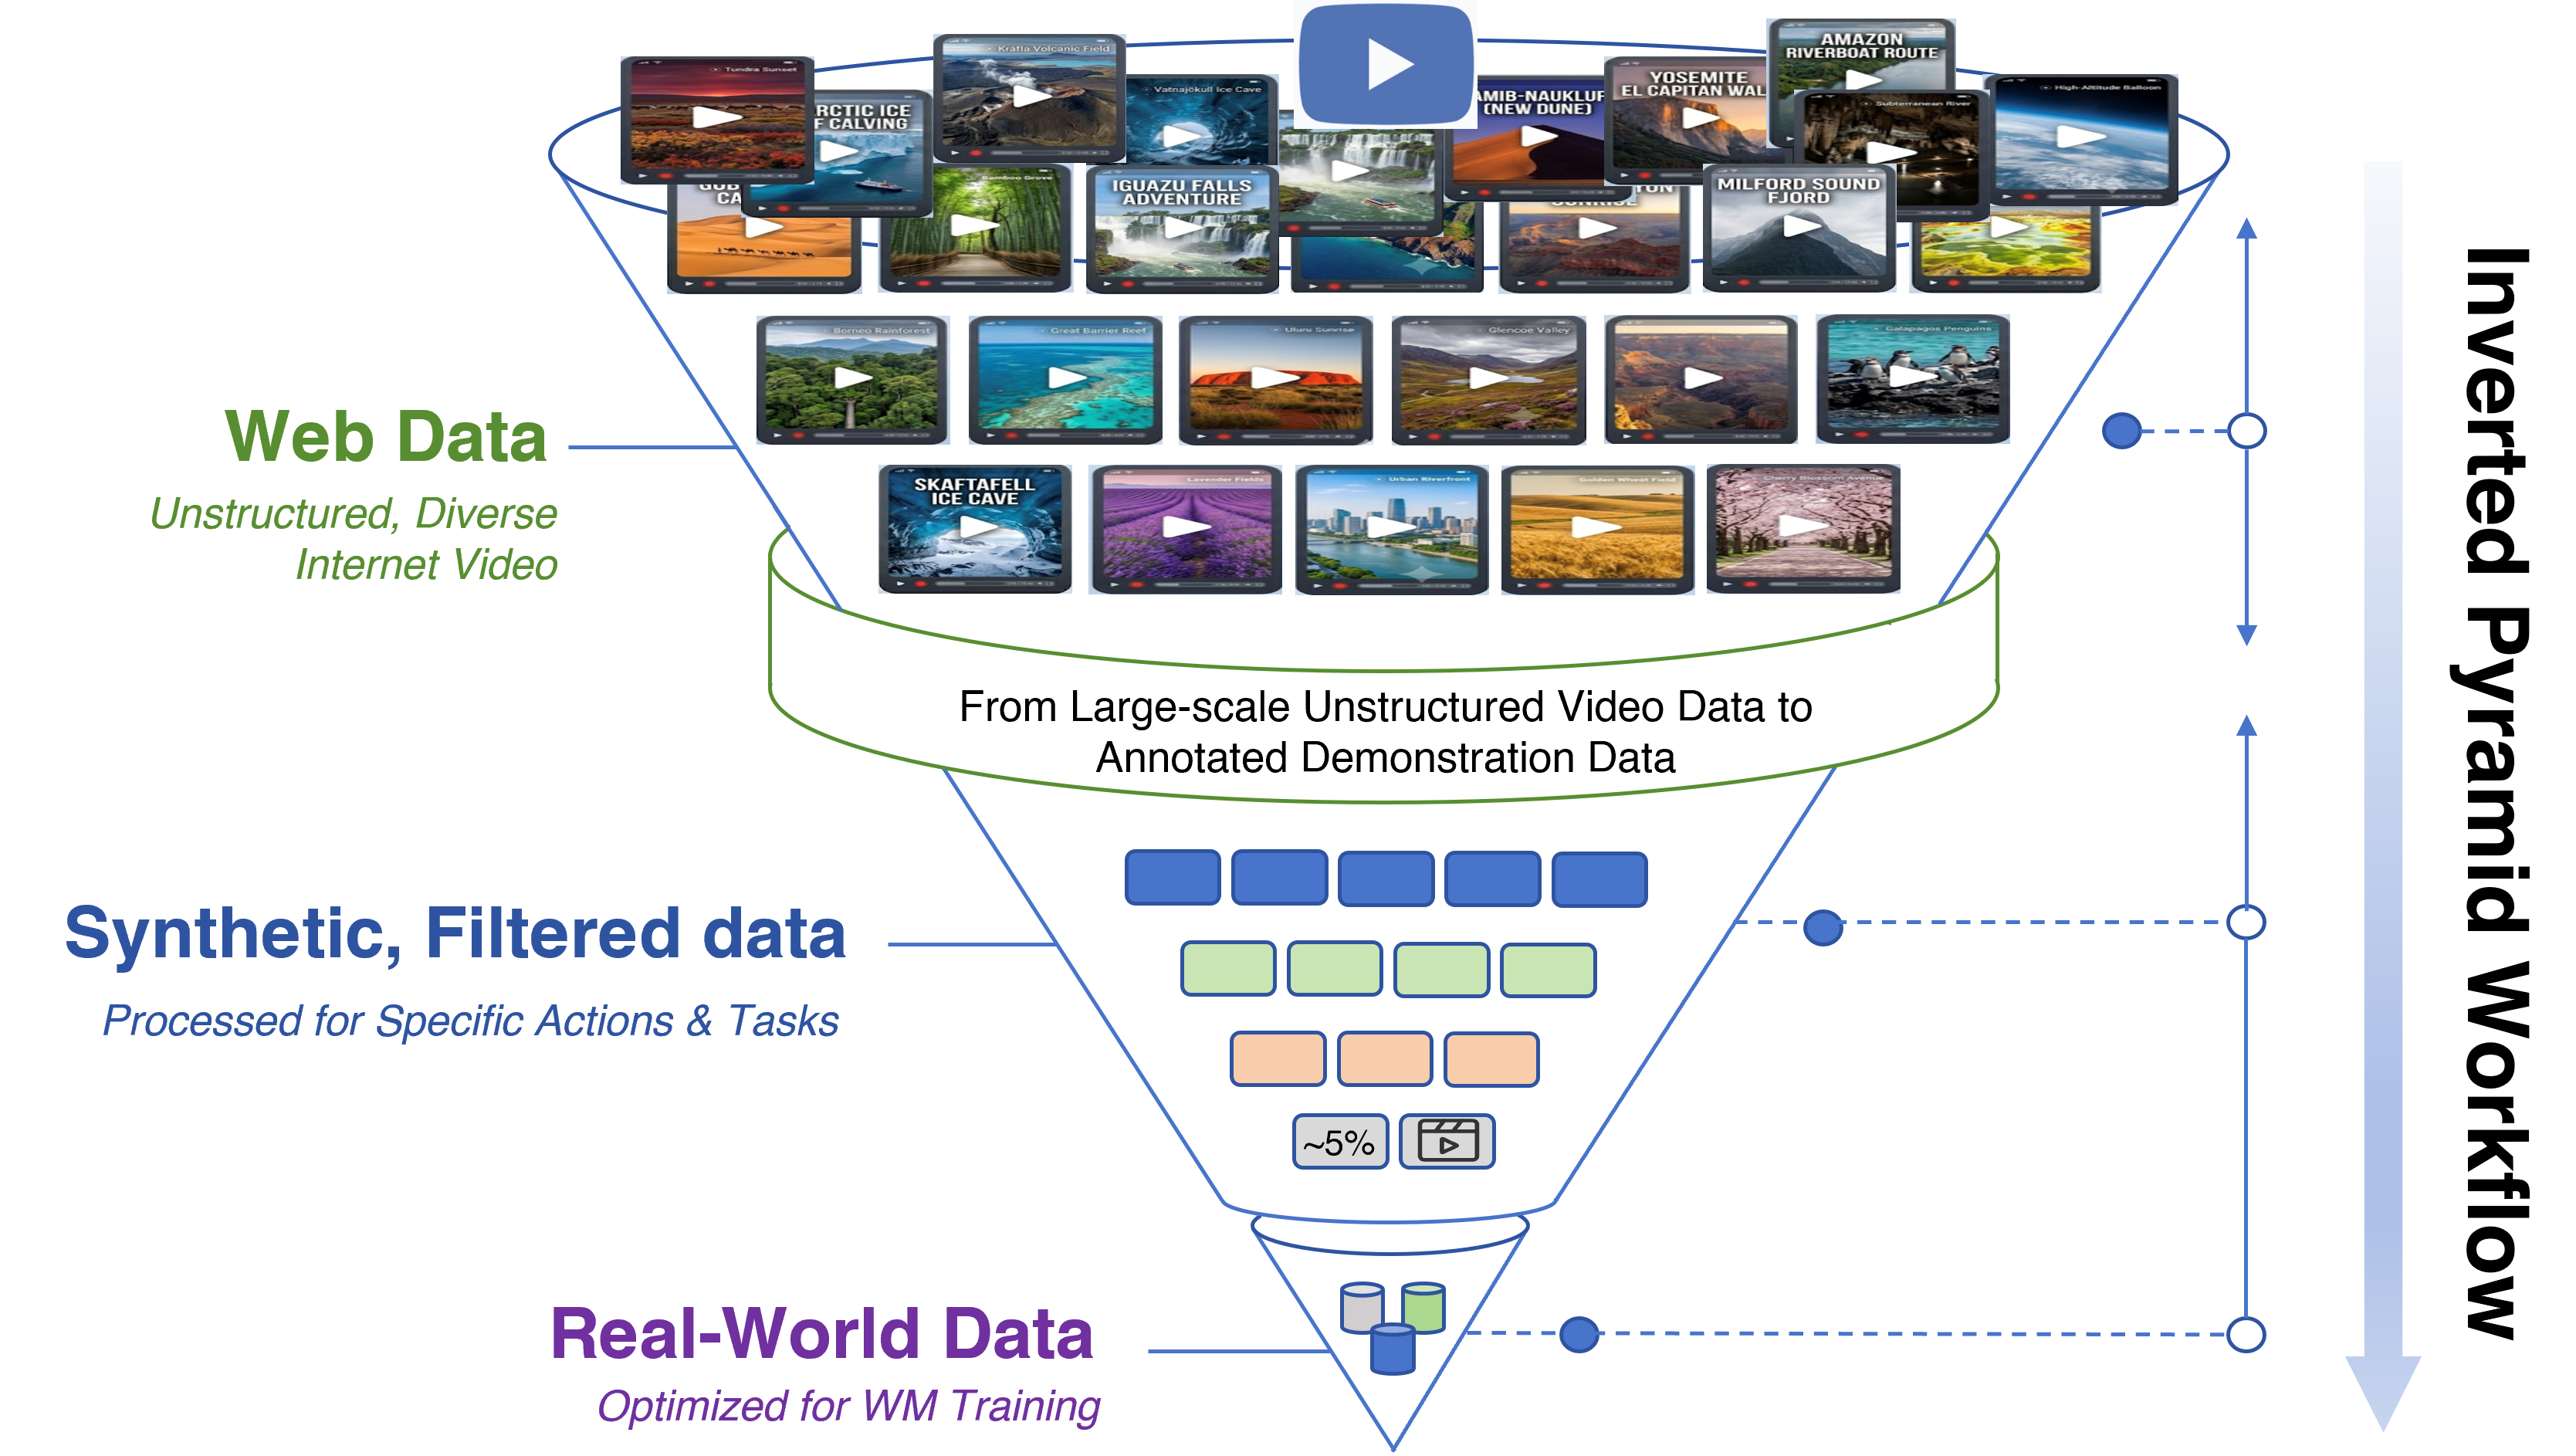
\includegraphics[width=0.85\linewidth]{figs/data4.png}
    \caption{用于机器人与物理世界模型训练的数据金字塔倒置漏斗：从海量无结构公共媒体，逐级提炼出规模紧凑、面向任务优化的机器人训练数据。最宽的顶层是“互联网数据来源”：无结构、多样化的公共视频，即数十亿段记录人类物理交互的原始像素流。中间层为“合成与筛选数据集”：经过大幅精简、为特定机器人行动与操作任务筛选及合成的数据子集。最窄的底端是“真实世界任务数据”：规模小、经过精心整理、为端到端机器人训练充分优化的数据集，其紧凑规模便于高效微调具身模型。}
    \label{fig:data1}
\end{figure}

\paragraph{作为压缩机制的世界模型}
高维视频观测主要由与任务无关的光度变化占据：视角、光照、纹理、传感器噪声和杂乱背景的变化，掩盖了底层物理规律。原始像素并不显式表征恒存性、因果性或约束，只编码表面外观，而不编码产生视觉信号的物理生成结构。因此，提取这些隐含物理先验需要一种专门设计的\textit{压缩机制}，将高维、含噪视频观测提炼为紧凑、有力且具有语义结构的表征。这种压缩的核心功能不仅是降维，而是有针对性地保留信息：准确保留下游物理推理与控制所需的结构化因果和物理信息，同时系统地舍弃原始像素数据中占主导地位、却与任务无关的光度变化。\textit{我们认为，这正是世界模型具有定义性、奠基性的任务；从根本上说，它严格属于压缩问题，而非生成或模拟问题。}生成和模拟是良好压缩表征所带来的下游能力，并非目标本身；世界模型的核心目标，是解决一个信息论问题：将高维感官数据中隐含的物理知识提炼为可用、紧凑的形式。


\section{什么是世界模型？}
\subsection{定义与主要性质}

\begin{figure}
\centering
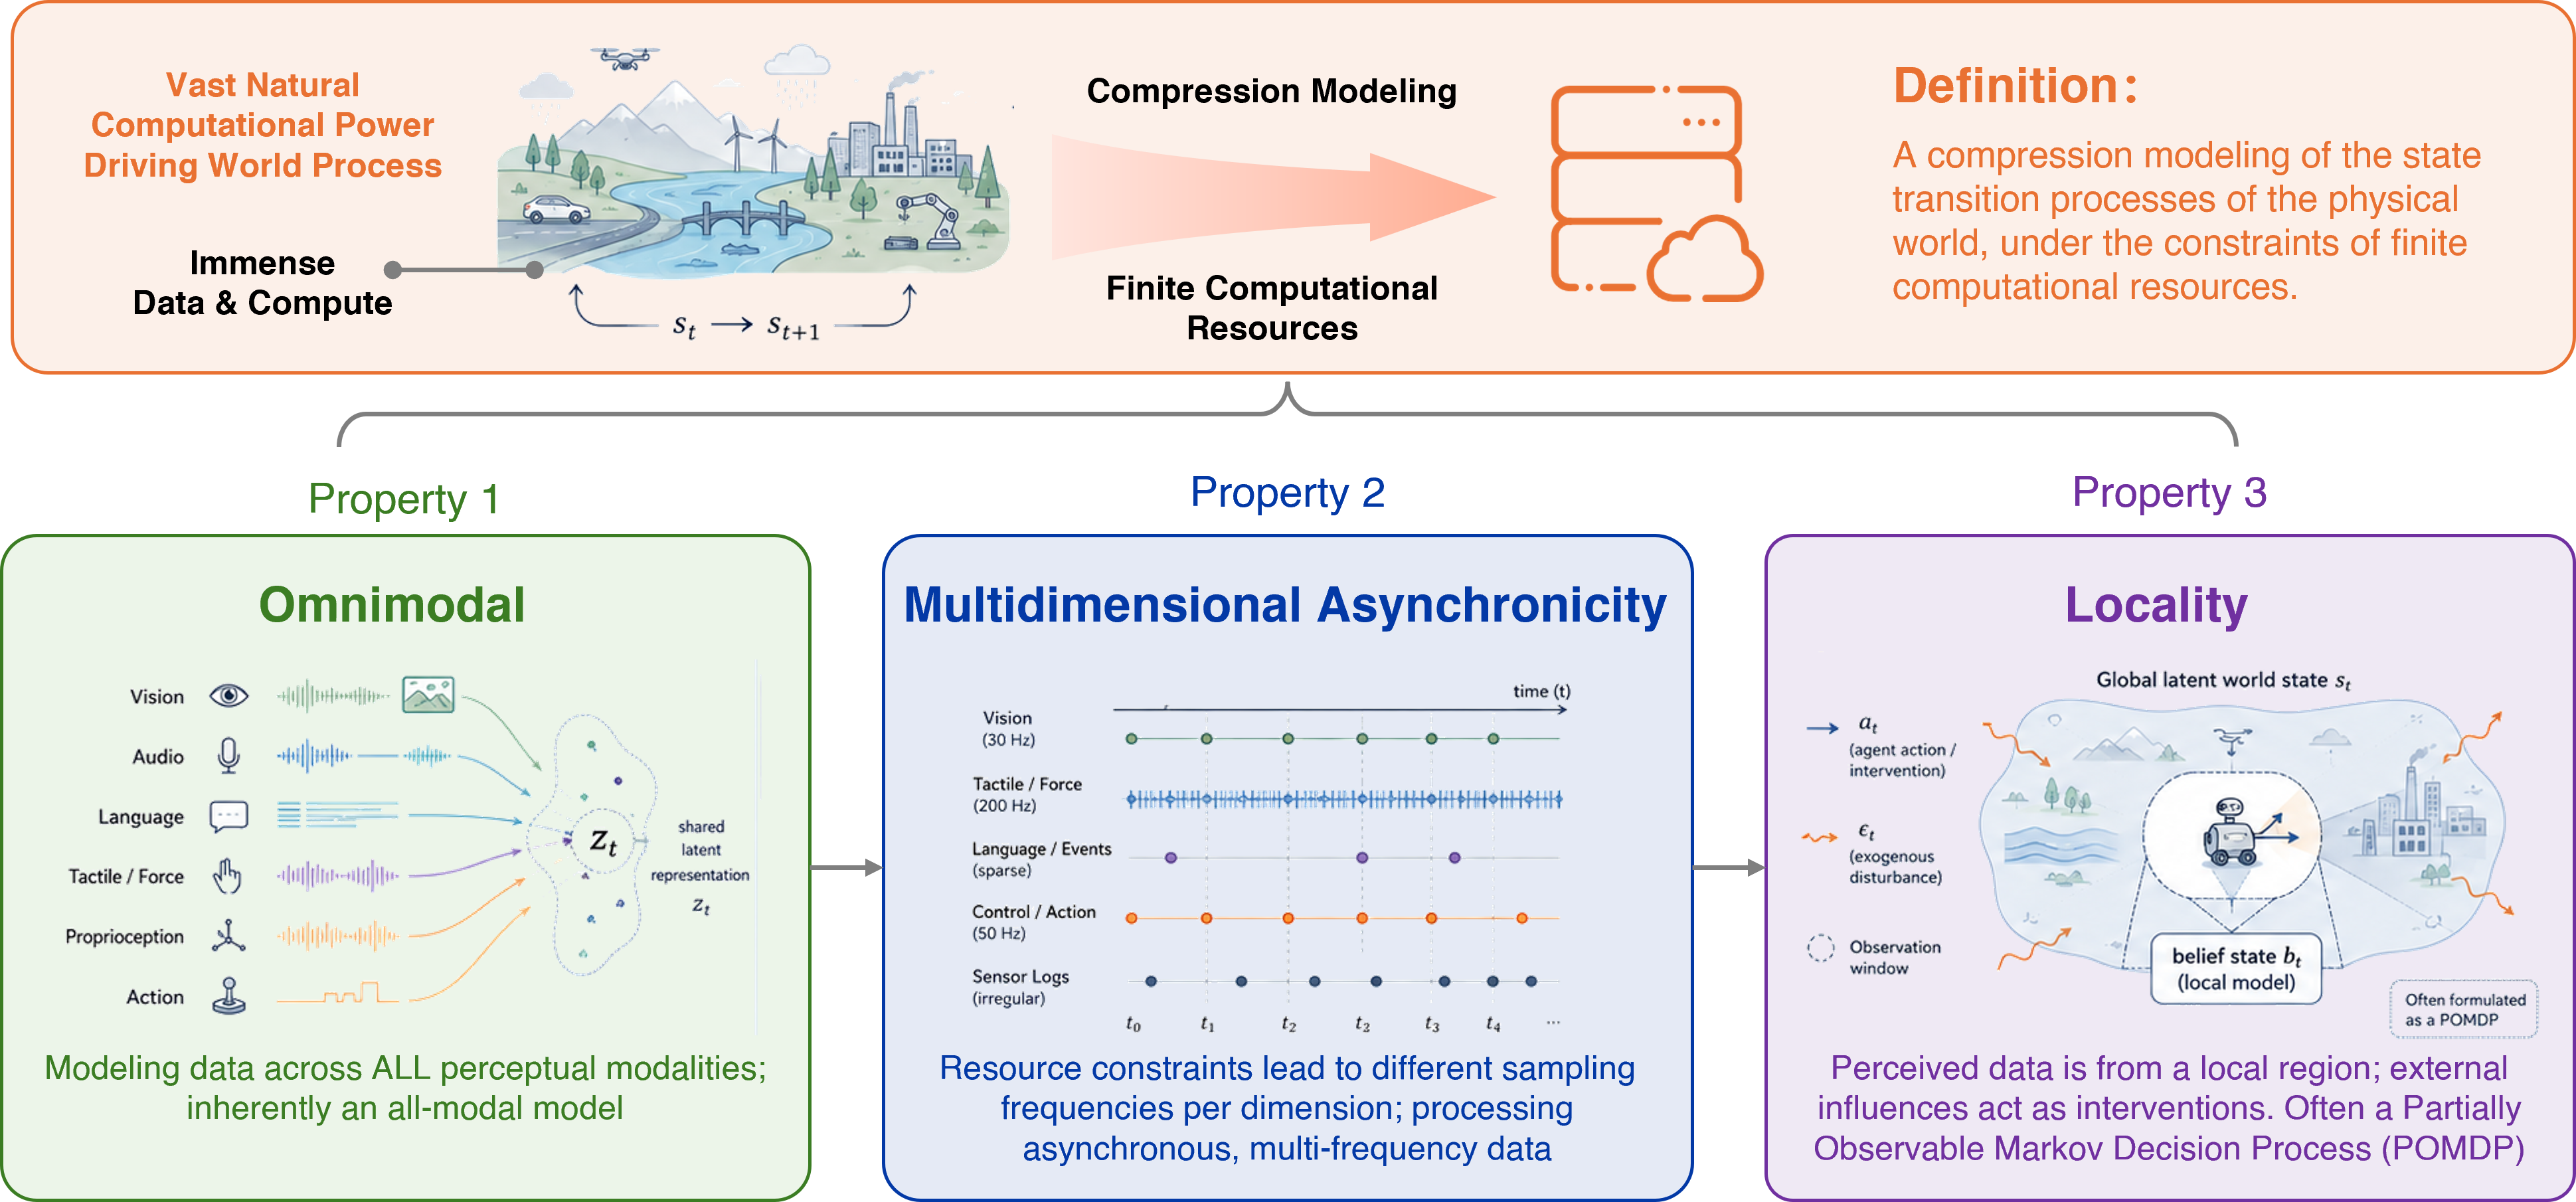
\includegraphics[width=\linewidth]{figs/WM-definition2.png}
\caption{世界模型的本质及其主要性质示意。}\label{fig:def-and-propoerties}
\end{figure}

本节专门从物理世界建模的角度，明确界定世界模型的概念，并概述其基本性质。

宇宙中一切物质与波的状态转移过程都客观存在，但驱动这些物理过程的自然计算能力极其庞大，难以估量。人类构建的系统无法复现这种无限复杂性，因此我们给出如下形式定义。

\begin{definition}[世界模型]
\label{def:worldmodel}
\textit{世界模型\footnote{依照这一定义，本文中的“世界模型”与“物理世界模型”（Physical World Model）含义相同，可以互换使用；但这并不意味着，在其他文献中，例如涉及交互式、三维几何一致的视频生成模型时，二者也具有相同含义。译注：原文此处写作“but this does mean”，与本句的转折关系及上下文不符，按“但这并不意味着”理解。}是在有限计算资源约束下，对物理世界状态转移过程进行的压缩建模。}
\end{definition}

如图\ref{fig:def-and-propoerties}所示，在这些内在计算约束下，通用物理世界模型具有三项主要性质：
\begin{itemize}
\item \textbf{全模态的作用范围（Omnimodal workscope）。}世界模型必须能够对所有感知模态的数据进行建模。它不限于文本或视觉，而在本质上是一种能够形成统一潜在表征的全模态基础模型。
\item \textbf{多维异步性（Multidimensional Asynchronicity）。}由于计算与感知资源有限，对物理世界各个维度的感知数据会以不同频率采样。因此，世界模型必须能够处理多维、异步（多频率）的序列数据。
\item \textbf{局部性（Locality）。}智能体的感知能力受资源限制，所采集的数据往往局限于某个局部区域。外部区域持续影响这一局部区域，构成干预。因此，从局部视角对世界建模，通常可表述为部分可观测马尔可夫决策过程（partially observable Markov decision process，POMDP）。
\end{itemize}

要理解这种局部、全模态近似的必要性，需要考察当前模型如何尝试回答关于现实的问题。当今人工智能领域占主导地位的世界模型，无论是潜在空间中的预测表征、用于游戏智能体的强化学习模型，还是用于具身模拟的视频预测模型，都遵循一种共同的生成式提问方式：给定当前观测，接下来会发生什么？真正的物理世界模型则重新界定了整个范式。基本问题从“将会发生什么”转向“正在发生什么、为什么会发生，以及将会发生什么”。这要求模型通过认识性推理（epistemic reasoning）\footnote{认识性推理是评估知识、信念及有理由支持的确信状态的逻辑过程，而非只关注世界的物理状态。它分析智能体如何依据部分观测、支持信息，以及关于其他智能体知道什么的元知识，构建、更新和评估内部表征。}理解物理系统的运行结构：发现系统自身的运行本体，识别离散的运行状态区间，确定正常与异常行为的边界，并刻画系统如何沿因果路径到达当前状态。

这一方法的意义，在于物理世界与数字世界有着巨大差异。数字数据一经产生，便可长期保持可读；多年前训练的语言模型，今天仍能回答量子力学问题。相反，物理系统内在地具有非平稳性，始终在变化。尤其是最重要的事件，如涉及安全的严重故障和罕见失效模式，可能从未出现在静态训练语料中。因此，静态世界模型不可避免地难以解决物理世界问题。我们需要一种架构，能够以通用基础表征为起点，自主、实时地适应各个应用中特有的物理规律。这样的动态系统应当具有\textbf{自洽性（self-consistency）}：当新的模态或数据通道进入时，世界模型仍能继续运行和演化，而不会面临崩溃。

归根结底，物理世界模型不仅是一台模拟引擎。它代表一种根本不同的智能形式：在局部观测与有限计算的约束下，深入理解物理世界、其持续演化及底层运行规律。

\subsection{智能体—环境循环}
\begin{figure}[t]
    \centering
    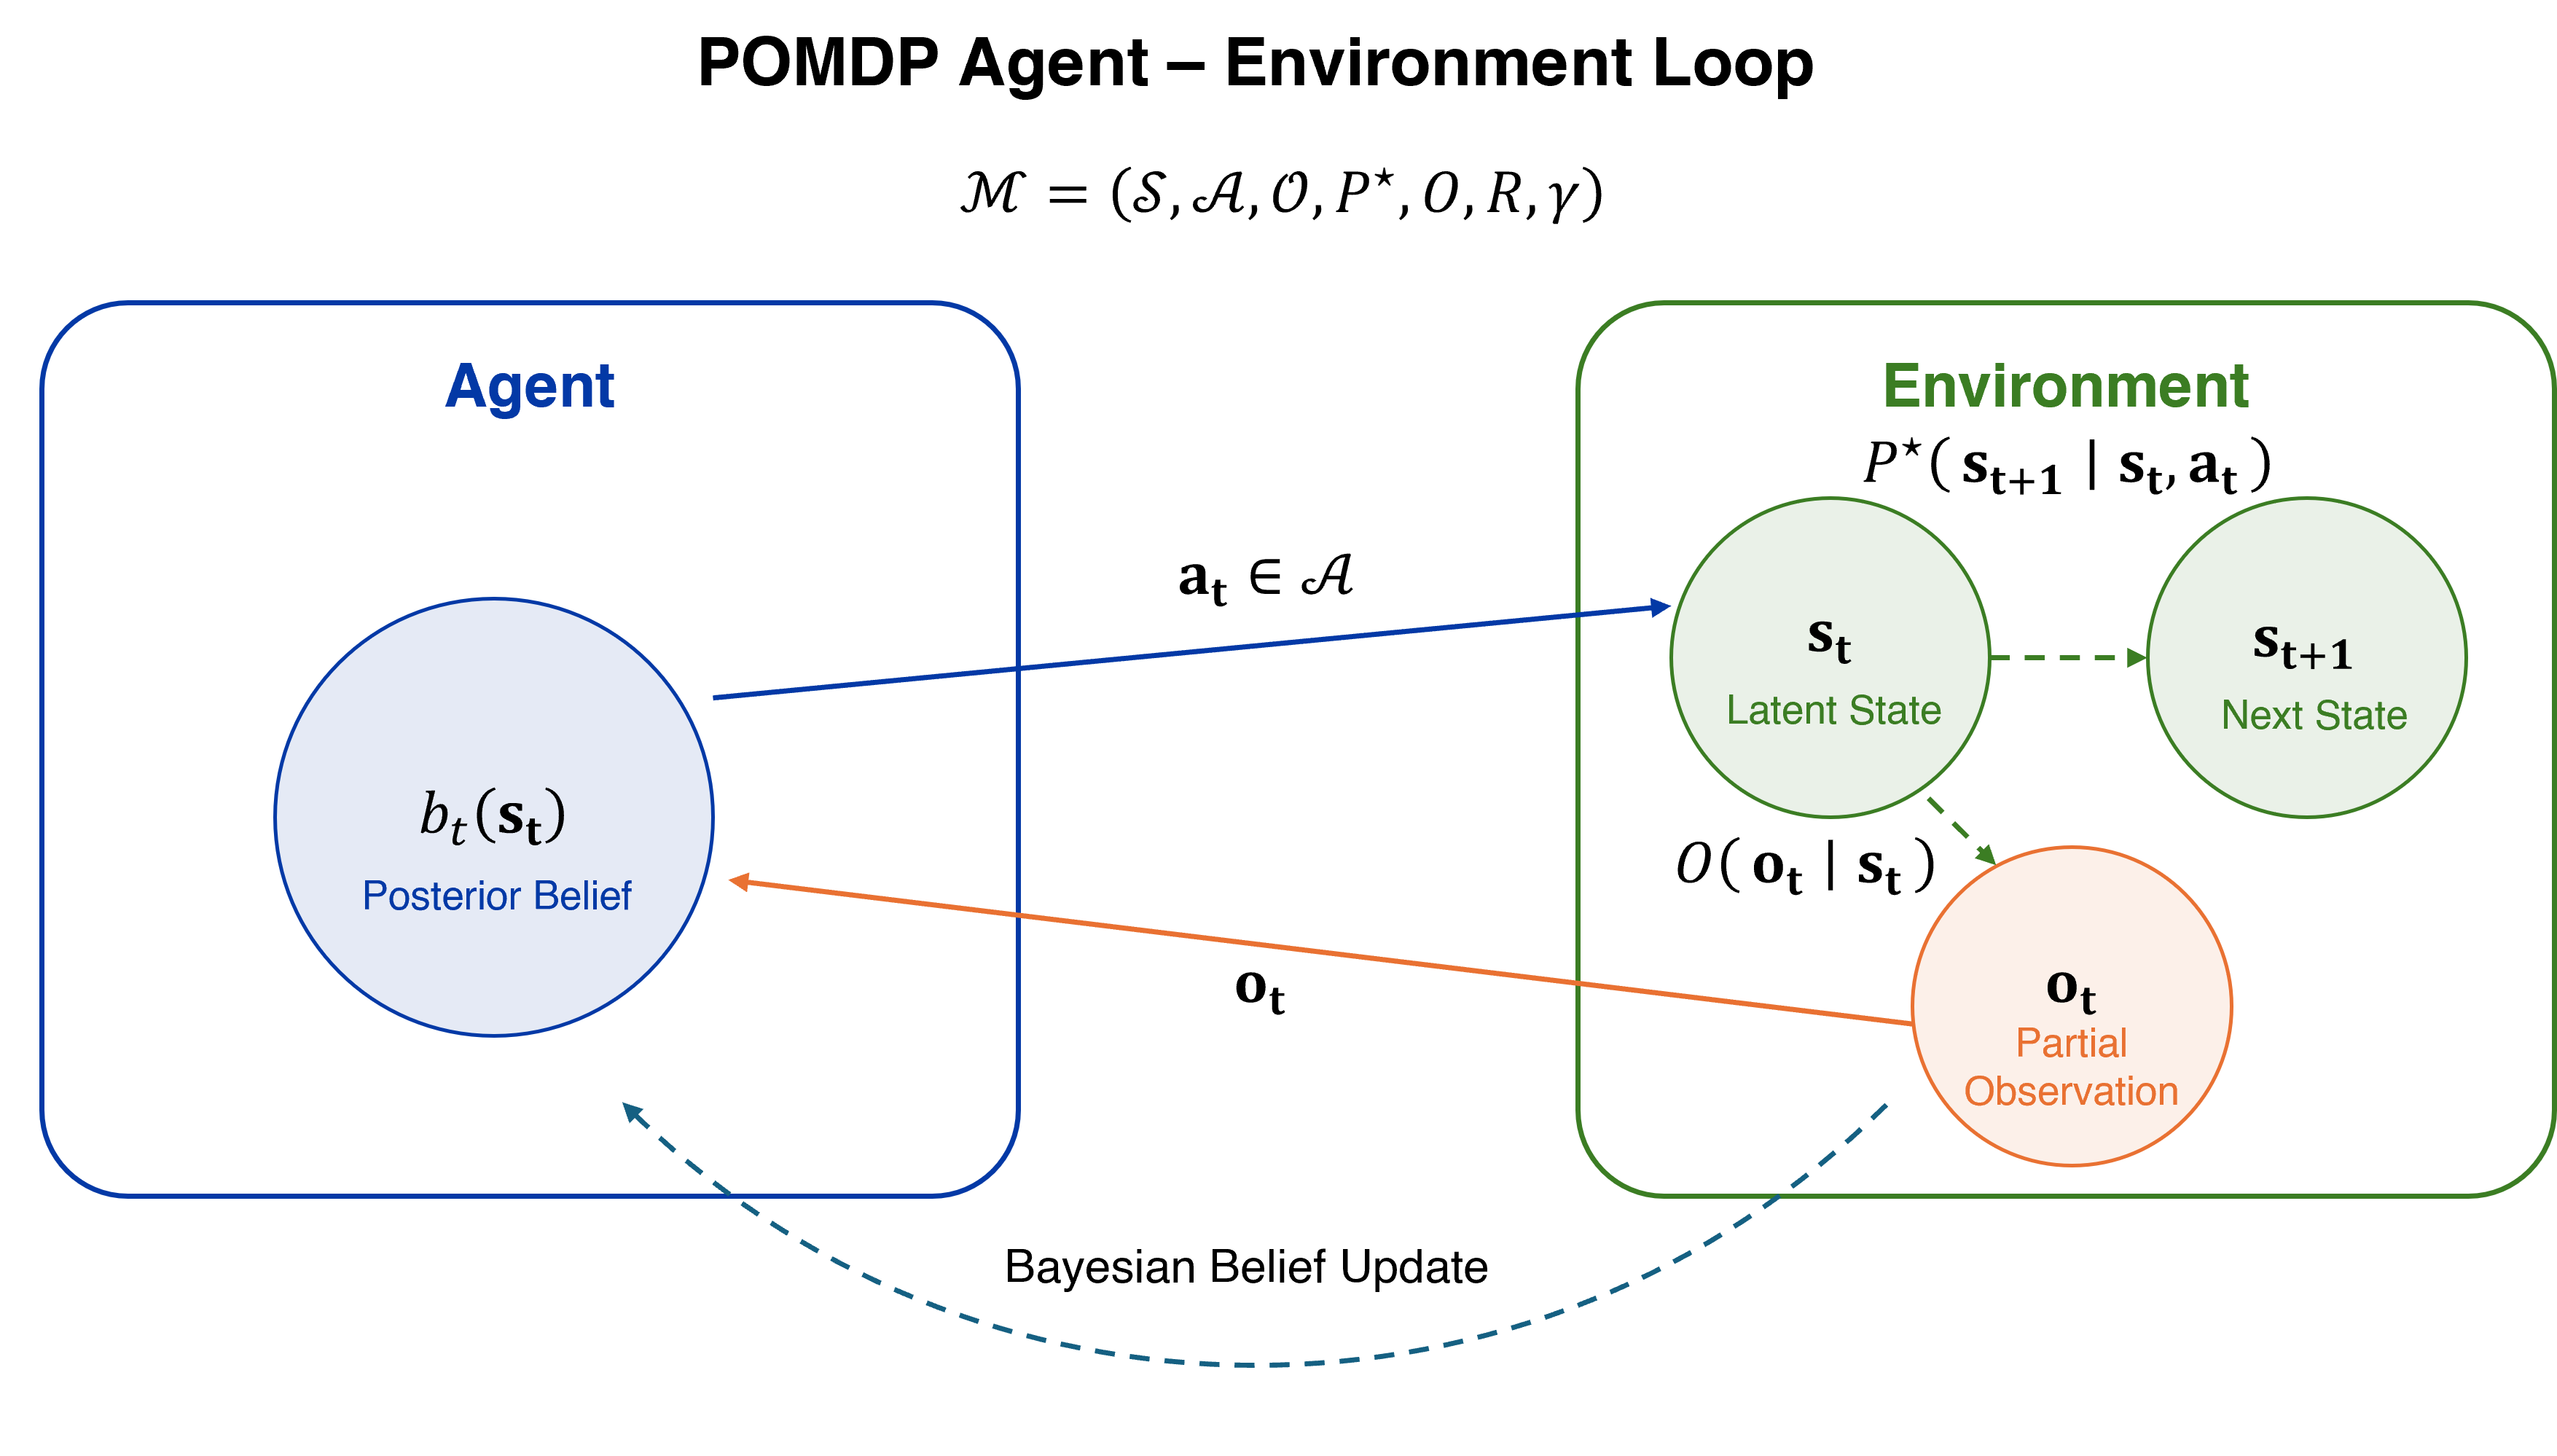
\includegraphics[width=0.8\linewidth]{figs/pomdp.png}
    \caption{采用本小节符号的POMDP智能体—环境循环示意。智能体维持后验信念$b_t(\mathbf{s}_t)$，选择行动$\mathbf{a}_t$；环境按照真实转移核$P^\star$演化，通过观测模型$O$产生部分观测$\mathbf{o}_t$；随后利用贝叶斯滤波更新信念。}
    \label{fig:pomdp-agent-environment-loop}
\end{figure}

一个在科学上有用的世界模型定义，应当从智能体与环境之间的序贯循环出发，而非从某个特定模型家族出发。自然的形式化方式是部分可观测马尔可夫决策过程（POMDP）$\mathcal{M}=(\mathcal{S},\mathcal{A},\mathcal{O}, P^\star,O,R,\gamma)$：环境处于潜在状态（latent state）$\mathbf{s}_t\in\mathcal{S}$，智能体选择行动$\mathbf{a}_t\in\mathcal{A}$，状态依照转移核（transition kernel）$P^\star(\mathbf{s}_{t+1}\mid \mathbf{s}_t,\mathbf{a}_t)$演化，智能体只能接收由观测模型$O(\mathbf{o}_t\mid \mathbf{s}_t)$生成的部分观测$\mathbf{o}_t\in\mathcal{O}$。真实状态通常是隐藏的，因此，有效行为不能只依赖原始观测，还需要对可能状态维持内部信念，并在新观测到来时更新信念。从这个意义上说，世界模型不只是像素、词元（token）或轨迹预测器，而是一个关于潜在状态、观测形成机制和行动条件动力学（action-conditioned dynamics）的内部模型，使智能体能够推断当前状况、想象接下来可能发生的事情，并在不确定性下评估干预。图\ref{fig:pomdp-agent-environment-loop}概括了这一循环及其核心变量。

这种表述也澄清了该术语的历史脉络。Craik早期的心智模型理论将智能理解为构建一种内部替代模型，在实际行动之前，先让它超前于现实运行\citep{craik1943nature}。Sutton的Dyna架构将这一思想转化为现代强化学习，把真实经验、模型学习、规划与行动显式地耦合在同一个循环中\citep{sutton1990dyna,sutton1991dyna}。近期的批评进一步强调：世界模型的目标不是穷尽式复现世界，也不只是生成视觉上可信的未来，而是为了有目的的推理和行动，模拟现实世界中可以采取行动的各种可能性\citep{xing2025critiques}。“可行动”这一限定至关重要。有用的世界模型不仅必须预测观测之间如何共同变化，还必须预测环境在干预下如何改变、哪些隐藏变量对控制重要，以及哪些不确定性仍未消除。在这一观点下，形式目标是学习一个对决策相关状态、转移与观测结构足够忠实的内部模拟器，使感知、反事实想象和策略选择都能在共同闭环中进行。

\subsection{理解与预测：世界模型的两种观点}
上述定义将物理情境下的世界模型界定为：在有限资源下对物理世界状态转移过程的近似，并强调全模态性、多维异步性和局部性三项主要性质。在这一定义之内，近期文献表明，“世界模型”一词有两种部分重叠、但哲学取向不同的含义\citep{ding2024understanding}。第一种观点主要将世界模型视为理解工具：它把感官数据压缩为持久的内部表征，揭示解释当前情境所需的实体、关系与机制。预测依然重要，但主要作为训练信号或一致性约束，促使表征捕捉正确的潜在结构。早期深度世界模型研究强调紧凑内部状态、记忆与潜在动力学，将其视为下游控制赖以建立的基础，体现的正是这一思想\citep{ha2018worldmodelsorig}。第二种观点主要将世界模型视为预测工具：根据模型向前推进世界、生成候选未来，以及为规划和决策提供前瞻的能力来评判它。LeCun的自主智能研究计划将这种预测式世界模型置于推理与行动的中心\citep{dawid2023autonomous}；Sora等大规模视频生成器则在可观测未来这一层面，使这种预测式理解尤为突出\citep{openai2024sora}。

这一区别会改变我们要求模型表征什么、优化什么、证明什么，因此十分重要。面向理解的模型通常偏好潜在抽象、以物体或关系为中心的结构、信念估计，以及对无关细节的不变性；其训练目标常强调表征学习、状态估计，或紧凑表征所具有的预测充分性；评估应检验所学状态能否为控制、解释和因果干预提供有用信息。面向预测的模型只要能够准确、可控地向前模拟，就可以容忍较弱的可解释性，因此常优先关注下一状态或下一观测的生成、长时域推演的持续可靠性、行动条件化，以及由外部标准判定的一致性。这两种观点也意味着不同的失效模式。模型可能推断出紧凑且与决策相关的状态，却生成视觉效果较差的渲染。相反，视频生成器可能生成极为逼真的未来，但如果不能保留隐藏状态、因果结构或干预含义，它仍无法成为控制所需的可靠模拟器\citep{xing2025critiques}。最强的系统最终将需要兼具二者：内部表征分离出恰当的潜在变量（latent variable），预测机制则将这些变量沿反事实未来向前推进。因此，这种分歧更适合被理解为：在特定架构中，哪种能力被视为首要能力，哪种被视为派生能力；而不是在两个不相容的定义之间做选择。

我们的观点是，对于物理世界模型，理解应当居于首位，预测应当服务于理解。无法识别潜在运行状态、因果结构以及与干预相关不确定性的模型，或许能够生成看似合理的未来，却仍不足以作为科学推理或具身控制的基础。另一方面，预测推演仍不可或缺，但其主要作用是通过反事实模拟检验并改进内部理解。从这个意义上说，最有用的世界模型并非单纯的未来生成器，而是把部分观测转化为可指导行动的理解，再利用预测支持决策的系统。

\subsection{功能分类：渲染器、模拟器与规划器}
区分面向理解和面向预测的世界模型，有助于澄清各自强调的能力，但尚未说明这些能力如何在行动系统中组织起来。因此，功能分类是有益的下一步：它根据世界模型在智能体—环境循环中的作用进行分解，而非按哲学侧重点划分。

李飞飞的功能分类可以重新表述为智能体—环境系统中三种互补的计算角色\citep{worldlabs2026taxonomy}。第一，渲染器是观测生成模型：以场景描述、交互历史或预期行动序列为条件，输出感知结果，最常见的是图像或视频。因此，它的功能是近似视觉上可信的观测分布，而非恢复环境完整的底层状态。第二，模拟器是承载动力学的模型，表征潜在或显式结构化的世界状态如何在干预下演化。它必须充分保留几何、物理约束、物体恒存性以及行动条件下的时间规律，才能支持可靠的前向预测。第三，规划器是决策模型，根据任务目标评估反事实未来并选择行动或行动序列。它不只是预测可能发生什么，还要决定应当追求哪一种可控未来。

这些角色自然地对应于POMDP闭环\citep{kaelbling1998planning}。真实环境状态不能直接获取，因此智能体对可能状态维持信念分布（belief distribution）。模拟器近似转移模型，在设想的行动下推进候选状态；渲染器近似观测模型，将这些状态投影为智能体随后可能接收的感官信息；规划器评估由此形成的、依赖信念的未来，以选择行动。选定行动执行后，环境产生新观测，修正智能体的信念并开启下一轮循环。因此，这三种功能既不是孤立模块，也不是相互排斥的模型类别。规划器查询模拟器，以比较行动后果，也可以调用渲染器，预期与任务相关的感知结果。反过来，规划器的干预决定环境的哪些方面变得可观测，从而产生可以改进感知预测与动力学估计的信息。它们的交互构成一个反复进行的推断、想象、干预与修正过程。

\begin{figure}
    \centering
    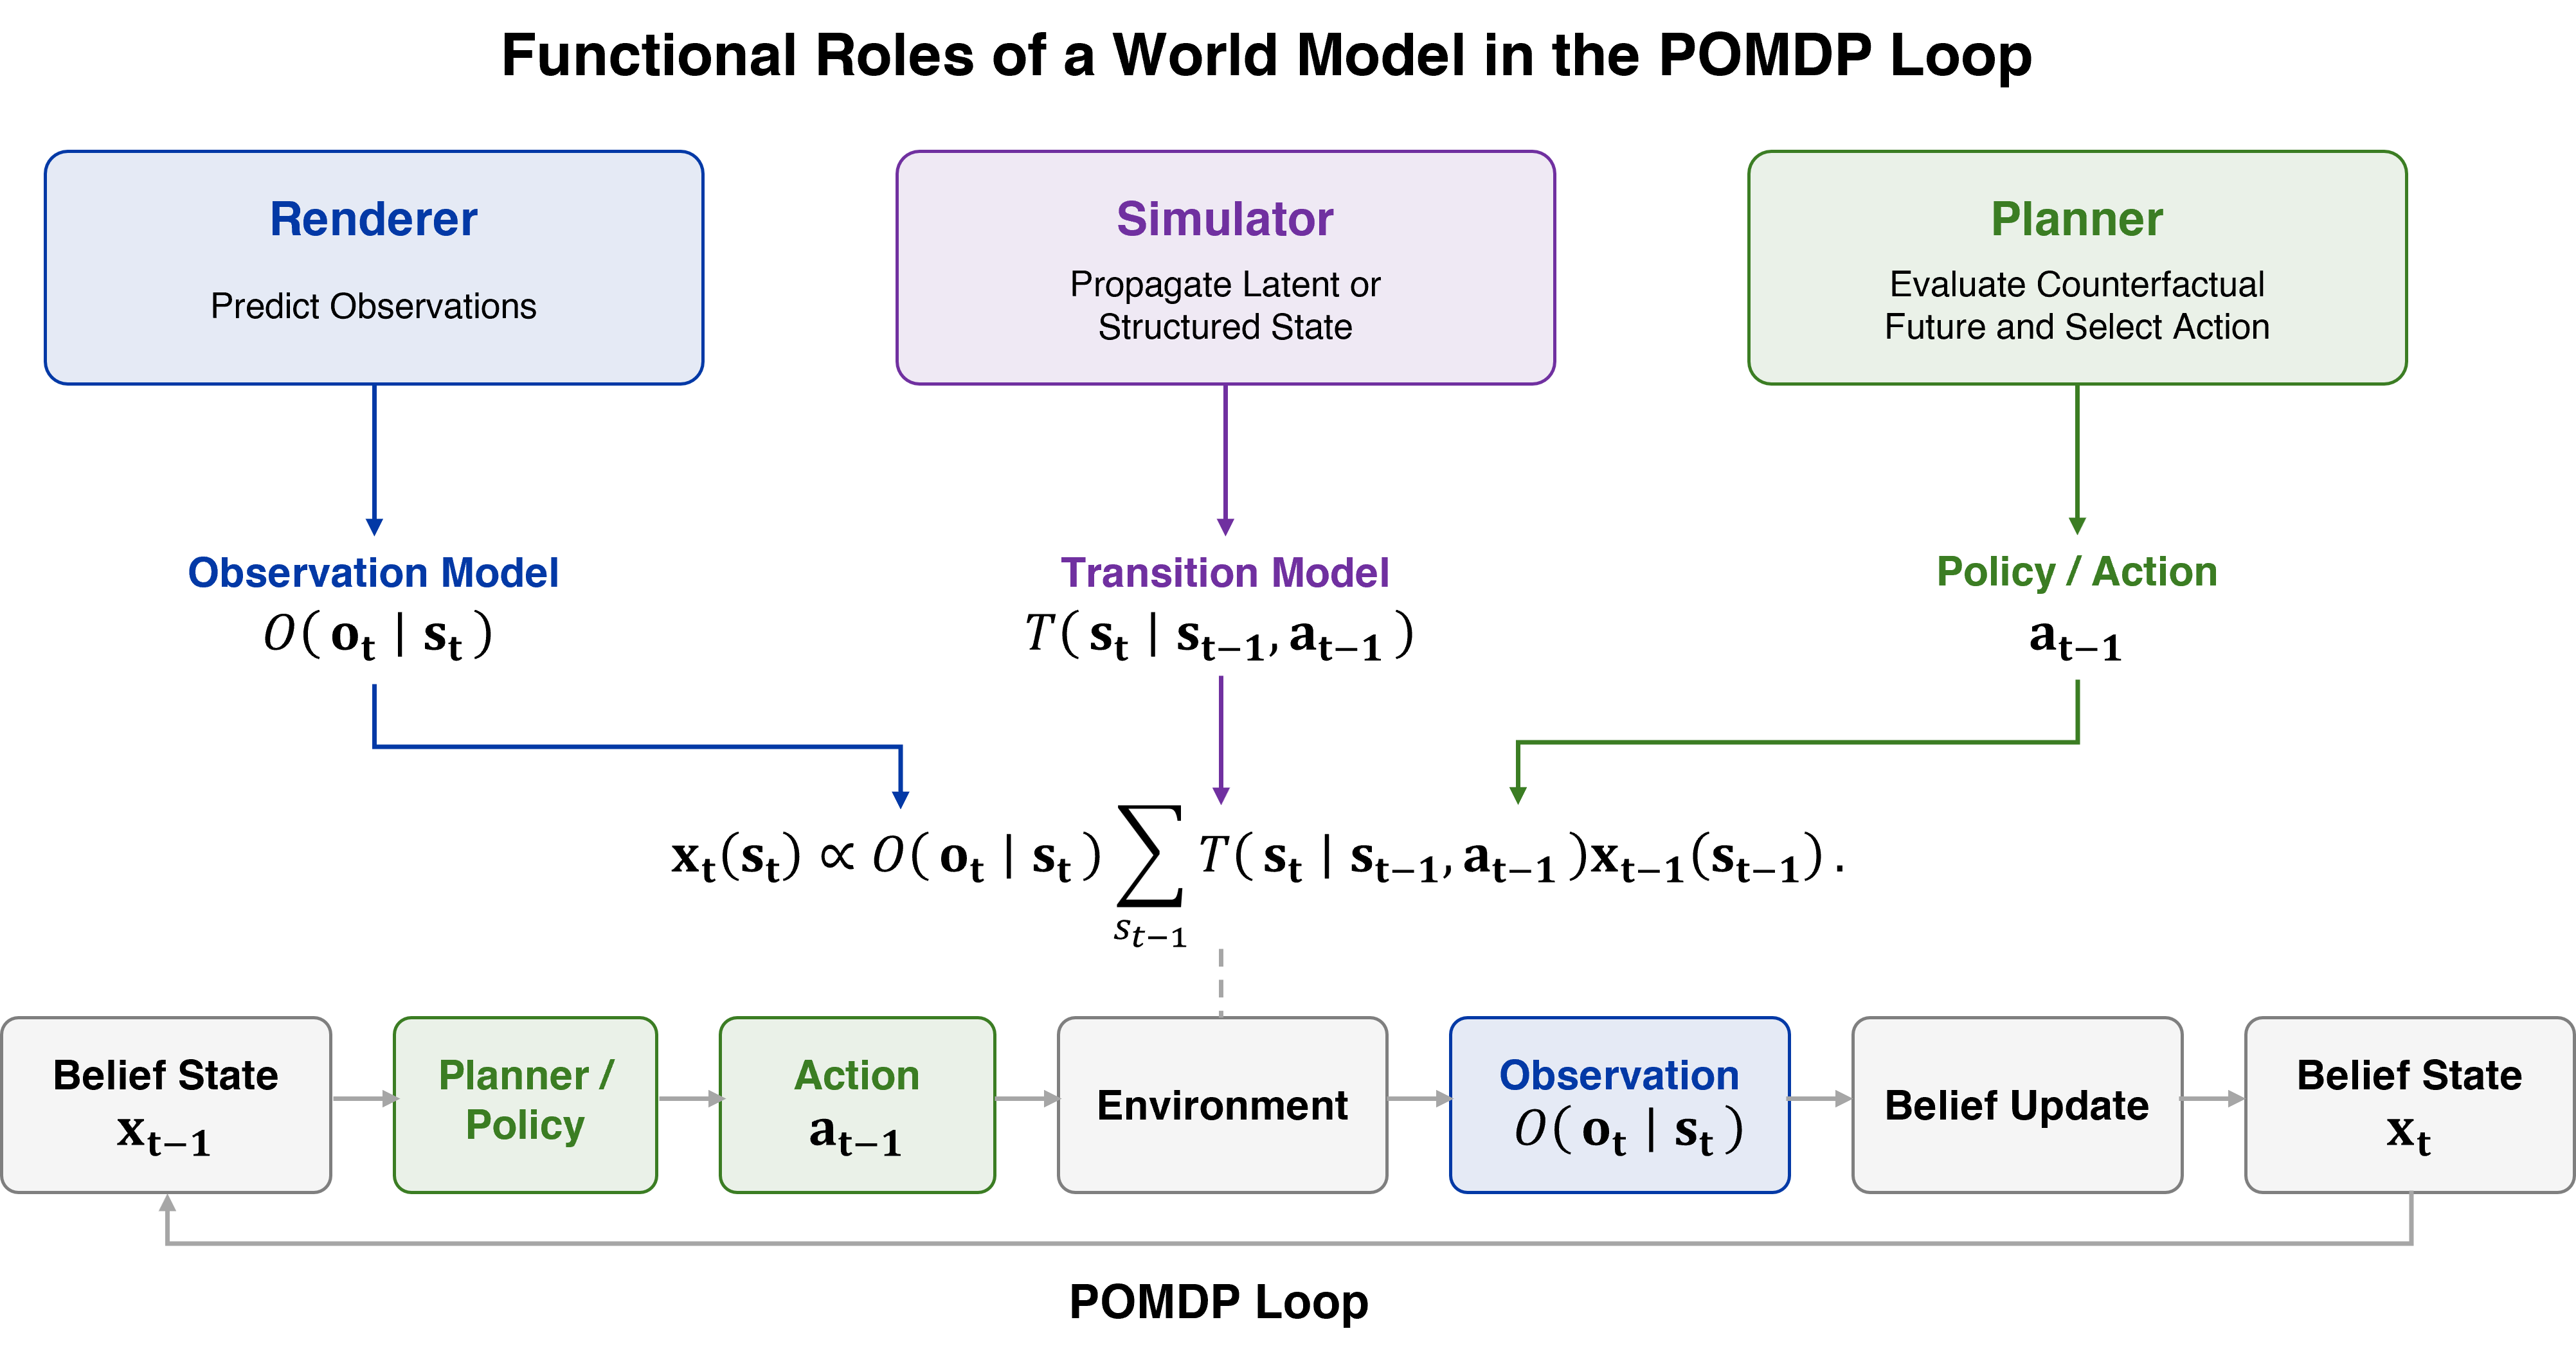
\includegraphics[width=0.96\linewidth]{figs/functional_roles3.png}
    \caption{世界模型在POMDP循环中的功能角色。}
    \label{fig:functional-roles}
\end{figure}

贝叶斯推断从规范角度解释了这一循环应当如何处理不确定性。在接收当前观测之前，智能体通过转移动力学传播上一时刻的后验，形成预测先验。随后，新观测按下式更新这一先验：
\begin{equation}
\mathbf{x}_t(\mathbf{s_t})\propto O(\mathbf{o}_t\mid\mathbf{s}_t)\sum_{s_{t-1}}T(\mathbf{s_t}\mid \mathbf{s_{t-1}},\mathbf{a_{t-1}})\mathbf{x}_{t-1}(\mathbf{s_{t-1}}).
\end{equation}
其中，$\mathbf{x}_t$表示后验信念，$T$是状态转移模型，$O$是观测似然。所得后验将积累的知识与当前信息结合起来，并显式保留不确定性，因此构成适当的决策信息基础。该后验随后又成为下一次预测先验的来源，使序贯贝叶斯滤波（Bayesian filtering）成为POMDP循环的推断支柱。理性规划应当在完整信念分布上优化期望效用，而非只考虑最可能的轨迹。因此，行动可以同时具有工具价值（instrumental value）和认识价值（epistemic value）：智能体可以为了实现外部目标而行动，也可以通过获取有信息量的观测来降低不确定性，或在两者之间权衡。先验编码跨环境学习得到、可重复利用的规律，后验使这些规律适应当前情境，反事实模拟则把二者与策略选择联系起来。因此，统一世界模型不应仅被理解为可能未来的生成器，而应被视为一个贝叶斯决策系统，持续地把不确定预测转化为依据观测信息、面向目标的行为。

\subsection{二维分类：功能与架构}
李飞飞的“渲染器—模拟器—规划器”分类与我们提出的分类处在不同的抽象层次。前者依据模型在智能体—环境循环中的功能角色分类：渲染器产生预测观测，模拟器在物理或动力学约束下推进世界状态，规划器依据目标选择行动。我们的框架则按模型的表征基础（representational substrate）与预测机制分类：观测层生成模型（observation-level generative model）直接在像素、视频等感知空间预测；潜在空间动力学模型（latent-space dynamics model）把观测编码为紧凑状态，并在表征空间中预测其演化；三维或其他结构化世界表征则显式建模几何、拓扑、物体、关系或物理属性。第一种分类问的是系统做什么，第二种问的是相关世界知识如何表示和计算。二者互补，而非相互竞争；一个模型通常应当在两个维度上各有一个或多个类别标签。

图\ref{fig:taxonomy}明确展示了这种多对多映射。Sora和Seedance位于观测层渲染器区域，因为它们对外提供的预测目标是视觉上可信的视频，而非结构显式、可独立查询的世界状态\citep{openai2024sora,gao2025seedance}。Genie 3的表征与输出仍位于观测层，但向三维世界表征方向延伸\citep{genie3}：它响应导航指令、智能体行动和可通过提示触发的世界事件，逐帧生成环境，从而支持交互式推演、反事实探索，以及智能体研究与训练。

JEPA家族位于潜在空间模拟器区域，因为其定义性预测目标是抽象的未来表征，而非重建像素\citep{assran2023ijepa,bardes2024vjepa}。VLA-JEPA将行动相关的潜在转移与连续行动生成耦合起来，从而把这一潜在预测机制扩展至规划器区域\citep{sun2026vlajepa}。Dreamer也位于潜在空间一列，但采用不同的生成式状态空间范式\citep{hafner2019dreamer}：从观测学习紧凑的行动条件动力学，并利用想象中的潜在轨迹训练演员（actor）与评论家（critic），以形成长时域行为。因此，在系统层面，它将潜在模拟器与通过想象训练的行动策略结合起来。更一般地，当行动条件潜在世界模型的预测与显式规划或控制目标耦合时，它们可以从模拟扩展至规划；用于以图像为目标的机器人规划的V-JEPA 2-AC，展示了这一点\citep{assran2025vjepa2}。

Marble主要位于三维／结构化表征区域\citep{worldlabs2025marble,kerbl20233dgaussians}。其高斯泼溅（Gaussian Splatting）表征支持高保真渲染与新视角合成（novel-view synthesis），碰撞网格则提供可供下游物理引擎使用、适于模拟的几何。因此，它连接了渲染与模拟，但不应将碰撞表征本身等同于完整的、学习得到的物理动力学模型。

Cosmos 3在图中表示为横跨多个区域的能力分布，而非分类中的单一位置\citep{nvidia2026cosmos3}。在共享的全模态架构中，其视听生成模式承担渲染器功能，行动条件前向动力学模式承担模拟器功能，策略模式则联合预测行动及其预期视觉后果。因此，图\ref{fig:taxonomy}中的位置反映了这样一个事实：不同的输入输出配置与后训练过程，可以从共享模型骨干中展现不同的功能角色。综合来看，对能力日益增强的世界模型，更合适的刻画方式是描述其运行配置与能力分布，而非将一个不可分割的模型名称归入单一类别。

出于同样原因，我们不把当前备受关注的世界行动模型（WAM）视为第四种实现类别。如图\ref{fig:taxonomy}中水平的WAM区域所示，WAM是用于具身决策、横跨多种架构的功能范式，而非与三列架构并列的表征基础。它的定义性特征是将预测式状态建模与行动生成耦合。在系统层面，WAM建模预期未来状态与行动之间的关系，即使这一关系通过级联分解实现，而非完全统一的网络。

WAM可以通过显式未来视频进行推理，如视觉规划流程；也可以通过紧凑的潜在未来表征或轨迹进行推理；还可以通过光流、三维点流、RGB-D轨迹等结构化空间表征进行推理。因此，它可以借助观测层、潜在空间或结构化世界模型实现。在李飞飞的功能维度上，WAM主要面向规划，但通常同时跨越规划器与模拟器功能，因为未来状态预测是行动生成的构成部分，而非仅仅起辅助作用。把WAM视为以预测式行动生成为中心的功能家族，可以避免混淆输出功能与实现基础，也允许对级联系统和联合系统进行有意义的比较：前者先预测未来状态表征，再导出行动；后者共同建模状态与行动轨迹。

\begin{figure}
    \centering
    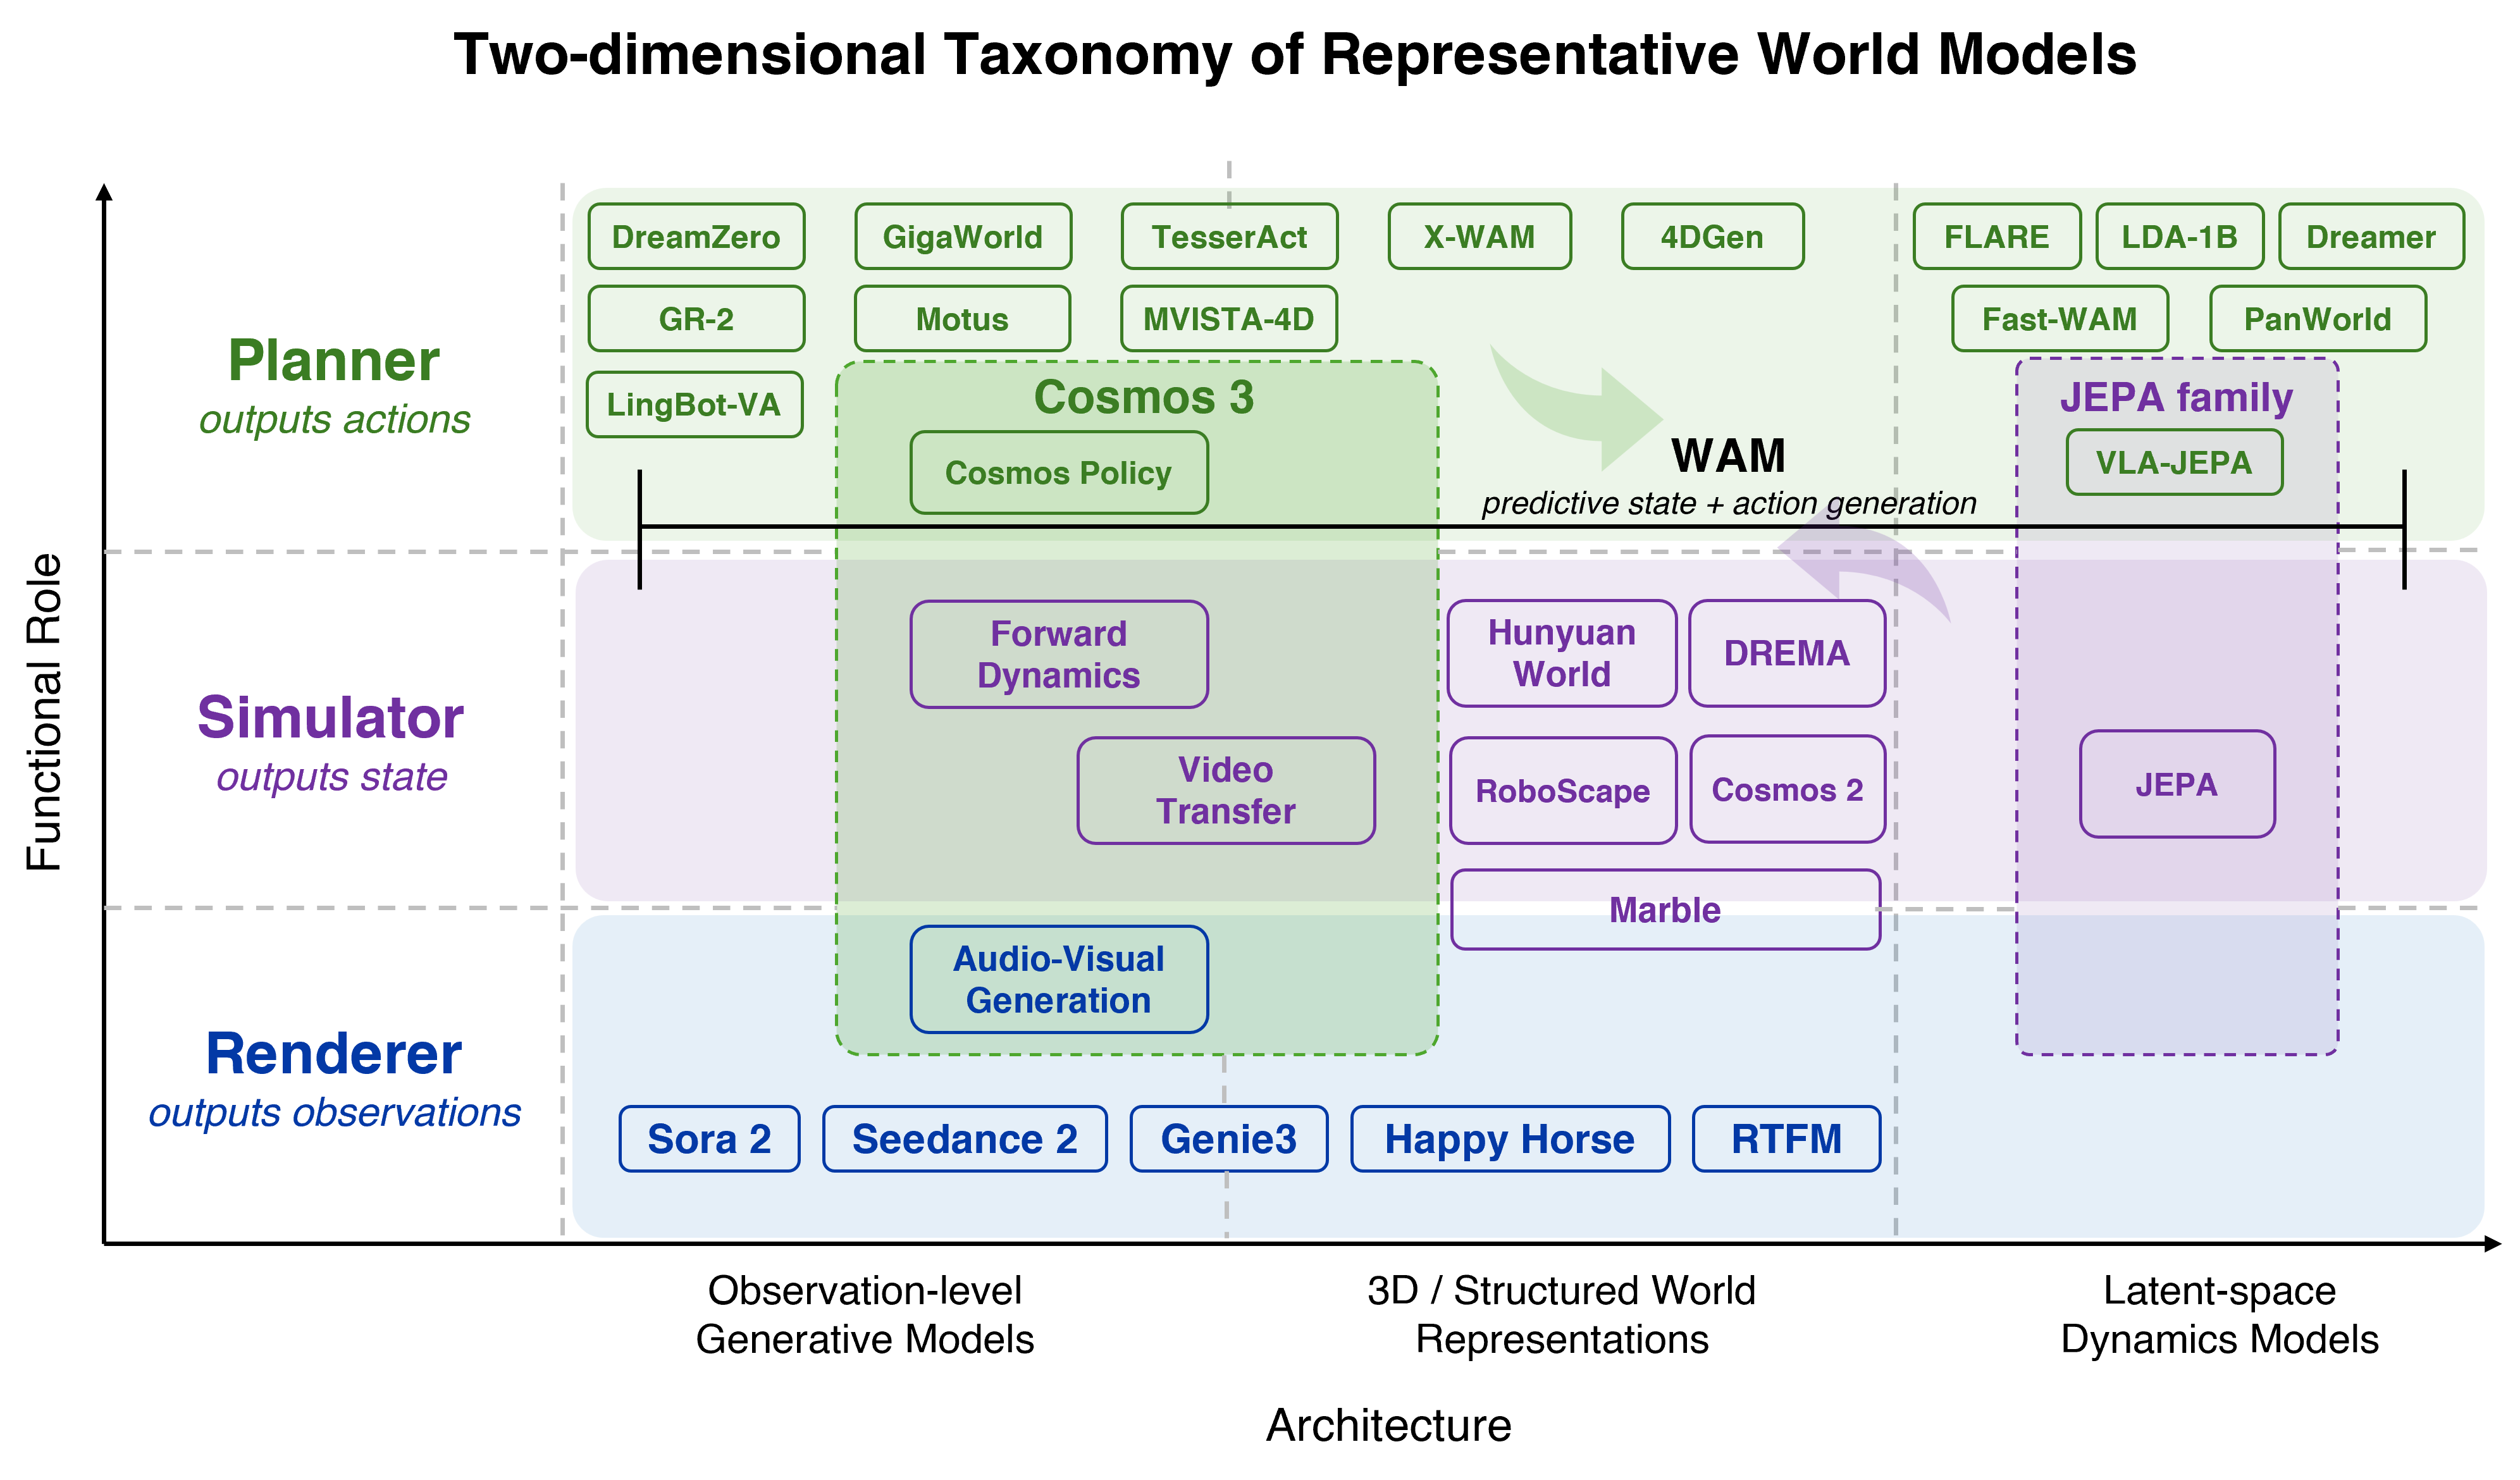
\includegraphics[width=0.96\linewidth]{figs/Taxonomy3.png}
    \caption{二维分类：功能与架构。}
    \label{fig:taxonomy}
\end{figure}

\subsection{将世界模型扩展到物理环境之外}
前述讨论主要仍局限于日常宏观环境，包括场景、机器人、车辆和可操作物体。更广泛的研究议程应当探讨：能否为科学领域构建类似的世界模型。在化学中，视任务而定，状态可以包括分子种类和结构、反应进程以及相关动力学或热力学变量；观测可以包括光谱、色谱或测得的产率；行动则可对应实验中可控的干预。在生物学中，相关状态可以通过层级或多尺度表征，跨越分子网络、细胞表型、组织及生物体层面的过程；干预可包括遗传扰动、给药及其他受控操作。在天文学中，潜在天体物理状态通过仪器被间接观测，而规划可能涉及根据天体物理动力学及仪器相关观测模型，选择观测目标、仪器与时间安排。

现有科学模型已经展示了这一表述的部分内容。在气象学中，GraphCast学习全球大气状态上的自回归转移模型，通过反复向前推进数百个大气变量，生成中期预报\citep{lam2023graphcast}。在本文分类中，它可被理解为结构化科学模拟器；但由于它不选择干预，也不闭合预测与行动之间的循环，因此不是智能体式世界模型。在分子尺度，MDGen学习分子动力学轨迹的生成模型，可以通过条件化用于前向模拟、转移路径生成及轨迹上采样\citep{jing2024mdgen}。它同样体现了学习式科学动力学建模，但本身不构成完整的实验规划系统。这些案例表明，即使没有明确使用“世界模型”这一名称，状态表征、时间推进、考虑不确定性的生成以及条件预测等世界建模组成部分，也已在各个科学领域涌现。在这些领域中，科学世界模型不能只生成看似合理的测量结果，还应捕捉机制性结构或其他具有科学意义的结构，在适用时遵守已知物理约束与不变量，量化不确定性，支持反事实干预，并在实际约束下帮助选择信息量大或效用最大的实验。完整的智能体式科学世界模型，还应把这些能力连接到实验循环：提出假说或干预，预测结果，执行实验，再依据新信息更新模型内部状态。

更广泛、也更具推测性的扩展，是有明确边界的社会系统\citep{zhou2025socialworldmodels}。我们将这一概念限制在参与者、交互规则、观测通道、干预空间和时间跨度都有清楚定义的系统，如小型团队、小型组织或界定狭窄的制度流程。这些系统可以建模为部分可观测的多智能体动力过程。候选潜在变量可以包括激励、信念、组织结构、资源约束和交互网络；观测可以包括通信、交易和绩效记录；干预可以包括任务分配、组织重构或协商达成的行动。在这些边界内，社会世界模型可以为团队协调与组织运营提供情景分析。

继续讨论之前，我们强调，本文的主要研究对象是物理世界的世界模型，而非社会系统。这里对社会领域的讨论，只是用来澄清适用范围和潜在局限的概念性扩展，不应被理解为本文的中心研究对象。

这种表述不应未经限定地扩展到国家、人口群体或全社会预测。大规模社会系统具有开放性、反身性和非平稳性，其规范性目标也存在争议：预测与干预可能改变被建模的行为，智能体可能对模型做出策略性反应，不同群体可能追求不相容的目标。此外，信念、偏好和意图等变量只能被部分观测，也可能依赖存在争议的理论假设。因此，当制度变化或公众知晓预测时，历史预测准确性并不能保证干预效果可靠。

其中的伦理与治理风险相当大。根据通信和行为记录推断潜在状态，可能助长侵犯隐私的监控；含有历史偏差的数据可能再现歧视或不平等的风险分配。模型输出用于分配机会、执行政策或塑造行为时，还可能产生施为性影响，形成自我强化的反馈循环\citep{perdomo2020performative}。因此，社会世界模型应显式表示不确定性，记录其因果与规范假设，并接受隐私保护、偏差审查、分布变化（distribution shift）测试和人工监督。它们应被视为有明确边界的决策支持工具，而非社会预言机；不应被用于不受约束的人口规模预测、大规模画像、自动化治理，或涉及个人和社会群体的高风险决策。

为避免术语泛化，“世界模型”这一名称应保留给以下系统：维持状态的内部表征，建模时间转移及适用时的干预条件转移，并生成可检验的预测。在这些限制下，二维框架仍可用于边界明确、具有操作性定义的社会领域。一个不受约束、试图建模整个国家或社会的模型，不应仅凭其规模或预测雄心，就被视为世界模型。

\section{架构范式}
沿着以表征为中心的世界模型观点，本节依据系统如何表示并推进世界状态，对现有系统进行分类。我们区分三类模型：直接在像素、体素或视频词元上预测的观测层模型，学习紧凑预测状态的潜在空间模型，以及引入显式空间、几何或实体层结构的三维增强模型（3D-enhanced model）或物体中心模型（object-centric model）。随后讨论跨范式统一的趋势，即在共享架构中整合生成、理解、交互，以及多模态（multimodal）信息与物理世界的关联。表\ref{tab:wm_architecture_comparison}概括了主要取舍与代表系统。

\subsection{观测层生成式世界模型}
观测层生成式世界模型将世界建模视为高维观测合成，直接预测未来像素、体素或视频词元。近期的大规模视频生成器，包括Sora类模型\citep{openai2024sora}、Wan\citep{wan2025wan}、Happy Horse\citep{happyhorse2026}、Seedance系列\citep{gao2025seedance,seedance2026seedance2}、Movie Gen\citep{polyak2024moviegen}、HunyuanVideo\citep{kong2024hunyuanvideo}、CogVideoX\citep{yang2024cogvideox}和Kling系列\citep{kling2025omni}，并不都属于严格的决策中心意义上的世界模型，但代表了从大规模视频学习物理先验的观测层路线。更明确具有交互能力的系统，包括Genie系列\citep{bruce2024genie,parkerholder2024genie2,genie3}、GameNGen\citep{valevski2025gamengen}、DIAMOND\citep{alonso2024diamond}和Oasis\citep{decart2024oasis}，则从被动续接视频迈向可控的环境生成。在物理与驾驶场景中，Cosmos\citep{nvidia2025cosmos}、GAIA-1\citep{hu2023gaia1}、DriveDreamer\citep{wang2023drivedreamer}、Drive-WM\citep{wang2023drivewm}以及Waymo World Model\citep{waymo2026worldmodel}进一步将观测层生成用于以轨迹、行动或场景为条件的模拟。

其主要优势在于规模：互联网视频提供了庞大的弱监督语料，可用于学习外观、运动、物体交互和场景动力学。因此，这些模型往往具有较高的视觉保真度，且覆盖广泛的现实世界现象。然而，视觉可信并不等于物理正确。像素空间模型生成的推演可能局部可信、整体却不一致；特别是在长时域中，物体恒存性、接触动力学、因果性或场景一致性方面的错误会逐渐积累。它们的计算成本也很高，因为预测发生在高维观测空间。因此，Diffusion Forcing\citep{chen2024diffusionforcing}、VideoPoet\citep{kondratyuk2024videopoet}、Wan\citep{wan2025wan}和Cosmos\citep{nvidia2025cosmos}等系统，探索如何把大型生成式视频模型的感知优势扩展到时间连贯的序列级预测。因此，评估观测层世界模型的核心标准不仅是感知保真度，还包括：在行动、指令、轨迹或其他条件信号下，所生成轨迹能否保持物理一致、因果连贯和可控。

\begin{table*}[t]
\centering
\setlength{\tabcolsep}{3pt}
\renewcommand{\arraystretch}{1.08}
\caption{主要世界模型架构范式的优势与局限。}
\label{tab:wm_architecture_comparison}
\vspace{.2cm}
\resizebox{\linewidth}{!}{
\begin{tabular}{@{} c | c | c | c @{}}
\hline
\textbf{范式} & \textbf{优势} & \textbf{局限} & \textbf{代表系统} \\
\hline
\makecell{观测层} &
\makecell{视觉保真度高；\\
输出直观；\\
可随互联网视频扩展} &
\makecell{生成成本高；\\
物理不一致；\\
长时域推演漂移} &
\makecell{\citep{openai2024sora}\\
\citep{bruce2024genie}\\
\citep{wan2025wan}\\
\citep{gao2025seedance}\\
\citep{nvidia2025cosmos}\\
\citep{chen2024diffusionforcing}} \\
\hline
\makecell{潜在空间} &
\makecell{高效想象式规划；\\
紧凑潜在状态；\\
适合扩展至长时域} &
\makecell{丢失关键细节；\\
难以目视检查；\\
目标不匹配} &
\makecell{\citep{ha2018worldmodels}\\
\citep{hafner2019planet}\\
\citep{hafner2019dreamer}\\
\citep{hafner2021dreamerv2}\\
\citep{hafner2023dreamerv3}\\
\citep{hansen2023tdmpc2}\\
\citep{schrittwieser2020muzero}\\
\citep{assran2023ijepa}\\
\citep{bardes2024vjepa}}\\
\hline
\makecell{三维／物体中心} &
\makecell{空间一致性更好；\\
物体级推理；\\
处理视角与遮挡} &
\makecell{需要结构化监督；\\
难以处理动态场景} &
\makecell{\citep{zheng2024occworld}\\
\citep{zhang2025robooccworld}\\
\citep{mildenhall2020nerf}\\
\citep{kerbl20233dgaussians}\\
\citep{worldlabs2025marble}\\
\citep{wu2023slotformer}\\
\citep{huang2025enerverse}} \\
\hline
\makecell{跨范式\\统一} &
\makecell{结合生成、\\理解、交互\\及多模态与物理世界的关联} &
\makecell{尚处早期；\\
模态对应关系问题；\\
行动保真度；\\
评估尚无定论} &
\makecell{\citep{liu2025lwm}\\
\citep{ge2024worldgpt}\\
\citep{zhou2025hermes}\\
\citep{ye2026dreamzero}\\
\citep{zhu2025uwm}\\
\citep{nvidia2026cosmos3}} \\
\hline
\end{tabular}}
\end{table*}

\subsection{潜在空间世界模型}
从像素空间转向潜在空间世界模型，不仅是效率提升，也反映了从视觉外观建模向任务相关状态演化建模的根本转变。PlaNet\citep{hafner2019planet}和Dreamer家族\citep{hafner2019dreamer,hafner2021dreamerv2,hafner2023dreamerv3}等早期潜在世界模型，利用循环状态空间模型（recurrent state-space model，RSSM）等潜在动力学模型，将高维观测编码为紧凑状态，并高效进行基于想象的规划。由于推演的是紧凑潜在状态，而非全分辨率像素，这些方法更容易扩展到长时域，更好地处理部分可观测性，也允许智能体在固定计算预算下评估更多假想未来。

除了效率之外，潜在建模还改变了世界建模的优化目标。潜在空间模型不必耗费容量重建每一处RGB细节，而可以聚焦于变化较慢、与决策相关、决定未来可控性的因素，如几何、物体关系、可供性（affordance）、接触动力学和时间演化。TD-MPC与TD-MPC2等基于模型的控制方法\citep{hansen2022tdmpc,hansen2023tdmpc2}进一步表明，规划可以直接在学习得到的、面向任务的潜在空间中进行，无需完整像素解码器即可高效优化轨迹。类似地，对比式及无重建世界模型\citep{kipf2019cswm,okada2022dreamingv2,poudel2023recore}表明，避免像素级重建，可以减轻对纹理、光照和细小光度变化等高频外观干扰因素的过拟合，从而提高鲁棒性。JEPA类预测表征学习等较新方法\citep{assran2023ijepa,bardes2024vjepa,assran2025vjepa2}通过预测表征而非像素，进一步质疑完整视觉重建的必要性。更广泛地，LDA-1B\citep{lyu2026lda1b}和Motus\citep{bi2025motus}等具身学习系统表明，有效策略往往可以从紧凑、面向任务的潜在表征中学得，而不必逼真重建整个视觉场景。从这个意义上说，潜在世界模型不仅可能更快，也可能更适合控制：保留低频、具有因果相关性的结构，同时抑制表面视觉细节，可以支持更鲁棒、更准确的决策。

不过，主要风险是过度抽象会丢弃视觉上很小、对决策却至关重要的信息，如夹爪与物体的接触、细小障碍物、微妙的物体姿态变化或形变。因此，核心挑战不只是压缩观测，而是学习一种潜在表征：舍弃外观噪声，同时保留决定未来可控性的因素。这也改变了评估方式：不能只按重建误差或预测误差评价潜在世界模型，还应检验其推演是否保留下游规划与控制所需的信息。

\subsection{三维增强与以物体为中心的世界模型}
三维增强和以物体为中心的世界模型，推动世界建模从单纯的帧预测转向结构化场景理解。传统视频模型可能生成视觉上可信的未来帧，但内部状态常难以解释，也可能不对应场景真实的三维布局。对具身人工智能而言，这构成了限制：模型还应支持对自由空间、物体位置、遮挡、视角变化、物体恒存性和物理合理性的推理。因此，近期研究探索了三维占据（3D occupancy）、鸟瞰图（bird's-eye view，BEV）表征、类似NeRF的辐射场（radiance field）、三维高斯泼溅，以及物体槽位（object slot），作为世界模型中结构更明确的状态空间\citep{mildenhall2020nerf,kerbl20233dgaussians,locatello2020slotattention,wu2023slotformer,zheng2024occworld,zhang2024bevworld,zhang2025robooccworld}。

一个方向是基于占据与BEV的世界建模。这些表征比像素更直接地揭示场景空间结构，因此有利于推理自由空间、障碍物、语义区域和未来场景演化。在自动驾驶中，OccWorld、OccSora、Drive-OccWorld和BEVWorld等系统，在占据或类似BEV的空间中学习未来场景动力学\citep{zheng2024occworld,wang2024occsora,yang2024driveoccworld,zhang2024bevworld}。在机器人学中，RoboOccWorld依据空间观测历史和未来相机姿态预测三维语义占据，将这种结构化状态观点扩展到室内具身预测\citep{zhang2025robooccworld}。这一家族的主要优势，是预测结果可以按空间位置查询，而不只是视觉上可信。

另一类方法使用连续或基于点的三维场景表征。NeRF和三维高斯泼溅提供具有几何信息的状态，支持新视角渲染与更强的视角一致性\citep{mildenhall2020nerf,kerbl20233dgaussians}。Marble、RenderWorld、GaussianWorld和GWM等近期系统，将这一思想扩展到持久三维世界生成、驾驶世界建模、流式占据预测及机器人操作\citep{worldlabs2025marble,yan2024renderworld,zuo2025gaussianworld,lu2025gwm}。与纯视频生成相比，这些模型能更好地跨视角、跨时间保留空间结构，但在动态场景和长时域交互方面仍面临困难。

以物体为中心的世界模型解决一个互补的问题：即使稠密的三维状态，也未必能分离出重要实体。OP3、C-SWM、Slot Attention、SAVi和SlotFormer等方法，学习物体或槽位层的表征与动力学，支持组合性更强的预测和推理\citep{veerapaneni2019op3,kipf2019contrastive,locatello2020slotattention,kipf2022savi,wu2023slotformer}。FOCUS和Object-Centric World Model for Language-Guided Manipulation等近期机器人系统，进一步将物体层抽象连接到操作及指令条件预测\citep{ferraro2023focus,jeong2025objectcentricwm}。这种抽象很有用，因为许多具身任务自然地围绕持续存在的实体及其关系定义，而非全局图像模式。

最有前景的方向，是结合这些表征，而非将其视为相互竞争的选择。占据表征支持自由空间与碰撞推理，NeRF和三维高斯表征支持视角一致的渲染，物体槽位则支持组合推理。EnerVerse和EnerVerse-AC等混合具身系统，通过连接多视角预测、记忆、四维场景表征、指令或行动条件化，以及具身未来生成，已经指向这一方向\citep{huang2025enerverse,jiang2025enerverseac}。更普遍的启示是，未来具身世界模型可能需要在共享物理表征中结合空间几何、时间记忆、物体结构及与交互的关联。

同时，加入三维结构并不会自动解决世界建模问题。模型可能准确重建空间，却仍无法捕捉可供性、因果性、物体恒存性或任务相关语义。物体中心模型紧凑且可解释，但在杂乱场景和遮挡下可靠地发现物体，仍然困难。NeRF或三维高斯模型可以渲染精细视图，但扩展到动态场景、长时域预测和闭环交互仍有挑战。因此，关键问题不是世界模型看起来是否更加三维，而是其状态是否构成对物理世界有用且连贯的表征。强大的具身世界模型，应具有几何一致性、时间上的持续一致性、物体感知能力和物理合理性，并能供下游推理、规划或控制模块使用。

\subsection{统一趋势：全模态世界模型}
\begin{figure}[t]
    \centering
    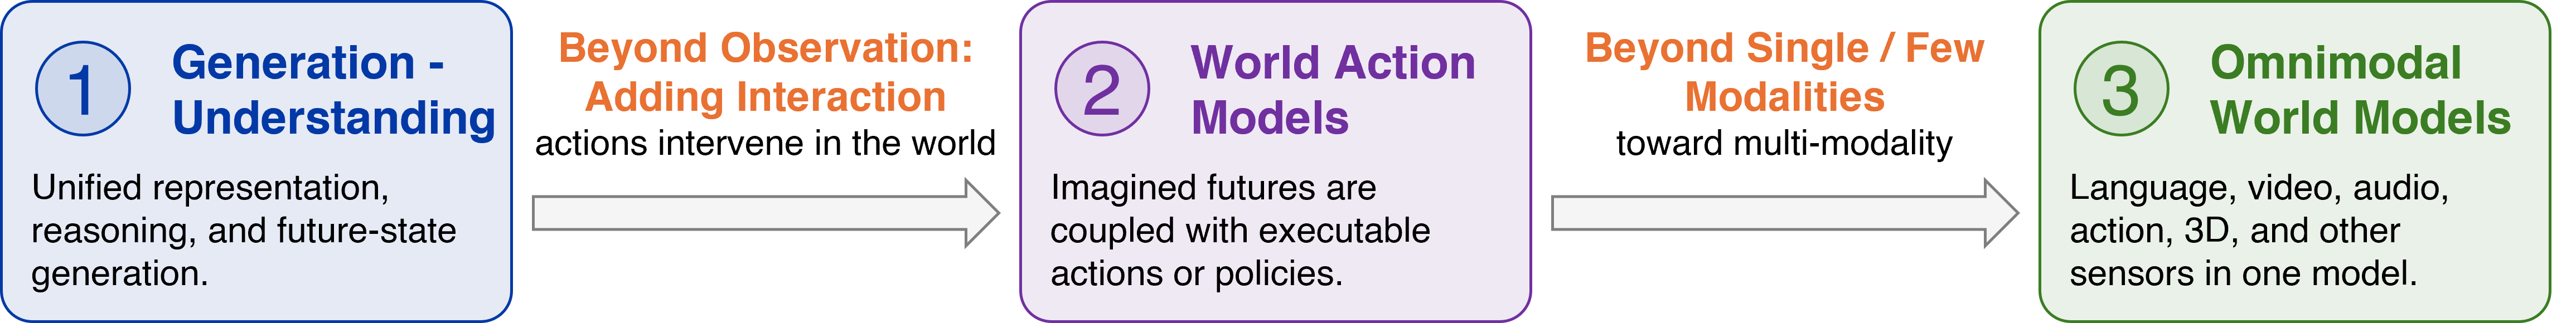
\includegraphics[width=\linewidth]{figs/omnimodal.png}
    \caption{世界模型架构的统一趋势。生成与理解统一模型首先通过引入交互及与行动的关联，超越被动观测，形成世界行动模型（WAM）。此后，该范式进一步超越单模态或少数模态建模，迈向全模态模型，在共享物理表征中整合语言、视频、音频、行动、三维结构及其他传感器信号。}
    \label{fig:omnimodal_world_model_trend}
\end{figure}

世界模型研究中逐渐形成一种共识：未来世界模型不应是纯生成器，而应是生成与理解统一的模型。世界模型不仅应合成未来观测，还应理解物体、空间关系、时间动力学、因果性和物理合理性。LWM\citep{liu2025lwm}、WorldGPT\citep{ge2024worldgpt}、HERMES\citep{zhou2025hermes}、HERMES++\citep{zhou2026hermespp}、GaussianDWM\citep{deng2026gaussiandwm}和UniDrive-WM\citep{xiong2026unidrivewm}等系统，更明确地体现了这一方向，尝试在统一框架中连接场景或视频理解与未来状态生成。相邻领域的多模态基础模型，如Chameleon\citep{chameleon2025}、Janus／Janus-Pr\citep{wu2024janus,chen2025januspro}和Emu系列\citep{wang2024emu3,cui2025emu35}，进一步表明理解与生成可以在共享的词元化或自回归架构中处理，为这一趋势提供支持。综合来看，世界建模正在超越视觉上吸引人的合成，迈向对动态世界联合进行表示、推理与生成的架构。

然而，物理世界不仅被观测，也承受行动。从部分可观测决策的角度看，具身智能体只能接收底层世界状态的部分观测，而其行动会干预潜在状态转移，塑造未来观测，如图\ref{fig:omnimodal_world_model_trend}所示。因此，仅统一生成与理解还不够。用于物理人工智能的世界模型，不仅应表征并生成未来状态，还应将想象的未来连接到可执行行动。这推动了世界行动模型（WAM）的出现\citep{wang2026wam_survey}，它们在共享生成框架中整合世界建模与行动或策略建模。WAM不再把动力学预测和策略学习作为独立模块，而是直接从视频—行动数据学习二者的耦合。例如，DreamZero\citep{ye2026dreamzero}表明，联合建模视频和行动，可以把世界模型转化为零样本策略；LingBot-VA\citep{li2026lingbotva}在自回归视频—行动框架中统一视觉动力学预测与行动推断；$\tau$0-WM\citep{zhou2026tau0wm}则为机器人操作整合行动生成、视频预测及未来状态评估。UWM\citep{zhu2025uwm}、Cosmos Policy\citep{kim2026cosmospolicy}、GigaWorld-Policy\citep{ye2026gigaworldpolicy}、Fast-WAM\citep{yuan2026fastwam}和Flash-WAM\citep{akbari2026flashwam}等相关系统，进一步探索视频预测与行动生成的不同耦合方式，包括联合扩散、以行动为中心的预测，以及无需在测试时显式想象视频的更快推理。这些模型共同标志着：研究正从被动世界模拟，转向既能想象物理未来，又能生成以这些未来为依据的行动的生成模型。

此外，世界模型正从单模态或少数模态场景扩展至全模态物理建模，在共享物理世界表征中整合语言、图像、视频、音频、行动、三维结构和传感器数据，见图\ref{fig:omnimodal_world_model_trend}。NVIDIA Cosmos 3\citep{nvidia2026cosmos3}是这一更广泛尝试的鲜明代表：它明确希望在混合Transformer架构中统一语言、图像、视频、音频和行动，从以视觉为中心的生成迈向通用物理人工智能后端。其他近期系统虽尚非完整全模态世界模型，也为这一方向提供了重要组成部分。Seedance 2.0\citep{seedance2026seedance2}探索以文本、图像、音频和视频为输入的统一多模态音视频生成；Wan／Wan2.1\citep{wan2025wan}提供可扩展的开放视频生成骨干；腾讯HunyuanVideo与HunyuanWorld系列\citep{kong2024hunyuanvideo,hunyuanworld2025}将视频生成扩展至可探索、可交互的三维世界构建；Kling-Omni\citep{kling2025omni}整合多模态指令遵循、视频生成、编辑与推理；Qwen-Omni\citep{qwen2025omni}则展示了如何在统一全模态基础模型中处理语言、视觉、音频和视频。综合来看，生成、理解、交互、空间推理和多模态物理预测，正在汇入共享的模型骨干。从这个意义上说，这一统一趋势源于物理人工智能的需求：用一个模型理解当下、想象合理未来、与世界交互，并整合多模态物理信号。

\section{训练与学习范式}
\begin{figure}[t]
    \centering
    \includegraphics[width=\linewidth]{figs/training-paradigm.pdf}
    \caption{世界模型主要训练与学习范式概览。}
    \label{fig:training-paradigm}
\end{figure}

\subsection{自监督与生成式预训练}
自监督与生成式预训练已成为世界模型的自然起点，因为在尚无任务奖励或密集专家标注时，它们便能把无标签经验转化为密集监督。令$\mathbf{x}_{1:T}$表示像素级观测或视频帧，$\mathbf{a}_{1:T}$表示行动，$\mathbf{c}$表示可选条件，$u_{1:T}$表示离散词元。共同目标不是为重建而重建，而是通过预测经验中被遮蔽、未来或下一个元素，获得紧凑信念状态（belief state）与转移先验。

视频预测是最直接的形式：
\begin{equation}
    p_{\theta}\!\left(
    \mathbf{x}_{t+1:t+K}
    \mid
    \mathbf{x}_{\le t},
    \mathbf{a}_{t:t+K-1},
    \mathbf{c}
    \right).
\end{equation}
它将表征学习建立在时间之上：持续存在、遮挡、接触、运动和场景变化，在每一帧都构成监督信号。然而，无行动条件的预测学习的是观测动力学，以行动为条件的预测才开始近似干预动力学——这一区别对规划至关重要。像素预测也是一个脆弱的替代目标：逼真画面既非可控物理理解的必要条件，也非充分条件。因此，现代系统越来越多地预测随机潜变量、词元化潜变量或扩散潜变量，将目标从渲染可信未来转向保留行动相关动力学\citep{finn2016unsupervised,ha2018worldmodels}。

掩码自编码（masked autoencoding）提供互补路线。MAE类目标根据可见上下文重建被掩蔽图块，视频变体则利用管状掩码（tube masking）与很高的掩码比例，发掘时间冗余\citep{he2022mae,tong2022videomae}。其有益作用在于压缩：编码器不能简单复制像素，必须从上下文推断结构。但重建只是替代目标。对世界模型而言，最好的掩码目标，应使潜在空间在干预下仍具有预测能力；这推动了JEPA类表征预测，在舍弃无关外观的同时，保留有利于规划的语义与动力学不变量\citep{bardes2024vjepa,assran2025vjepa2}。

下一词元预测（next-token prediction）提供了最易扩展的生成接口。视频、行动、语言、地图、本体感觉（proprioception）和奖励一经词元化或嵌入，预训练便可以最小化
\begin{equation}
\mathcal{L}_{\mathrm{NTP}}
=
-\sum_{t=1}^{T}
\log p_\theta\!\left(
u_t \mid u_{<t}, \mathbf{a}_{\le t}, \mathbf{c}
\right).
\end{equation}
这使世界建模能够借助Transformer的规模扩展，并支持多模态提示。GAIA-1将自动驾驶世界建模表述为离散词元序列预测；Genie则结合时空视频分词器（tokenizer）、自回归动力学模型，以及从无标签视频训练得到的潜在行动模型\citep{hu2023gaia1,bruce2024genie}。隐藏的瓶颈在于词元化：词元定义了模型的本体，而分词器舍弃的几何、接触或可控性信息，无法仅靠扩大规模恢复。

尺度定律将这些目标转化为系统问题。一种有用的抽象是
\begin{equation}
\mathcal{L}(N,D)
\approx
\mathcal{L}_{\infty}
+
A N^{-\alpha}
+
B D^{-\beta},
\qquad
C \approx \kappa N D,
\end{equation}
其中$N$是模型规模，$D$是训练数据，$C$是计算量。语言模型研究表明，扩大规模能带来可预测的幂律改进，而计算最优训练要求平衡参数量与词元量\citep{kaplan2020scaling,hoffmann2022training}。但对世界模型而言，$D$不应只理解为词元数量，还应理解为对状态、行动、机器人本体（embodiment）、视角、接触、罕见事件和时间跨度的覆盖。具身预训练的早期研究发现了类似的尺度行为，但其系数受到分词器、任务与架构的影响\citep{pearce2024scaling}。因此，仅有似然还不够：可扩展世界模型还必须按闭环一致性、可控性、长时域持续可靠性，以及对罕见运行情形的鲁棒性来评判。

因此，合成数据是扩展规模的实用途径。Omniverse Replicator和Isaac Sim等平台支持基于物理的合成数据生成；Cosmos-Drive-Dreams和GR00T-Dreams等近期流程，使用世界基础模型生成可控驾驶场景或合成机器人轨迹\citep{nvidia2022replicator,nvidia2025cosmos,nvidia2025grootdreams}。它们最有力的作用不是替代现实，而是扩展现实经验：真实数据确定分布的依据，模拟与生成式合成数据生成（synthetic data generation，SDG）则提供长尾、危险和反事实情形。核心问题在于校准：如何混合真实、模拟和生成数据，使更广覆盖改善物理泛化，而非让模型学到模拟器伪影。在这一观点下，预训练教给模型的不是如何渲染世界，而是智能体能够借以改变世界的那些变量。

\subsection{基于模型的强化学习}
\label{sec:mbrl}
基于模型的强化学习（MBRL）\citep{moerland2022modelbasedreinforcementlearningsurvey}，是最早赋予世界模型以决策为中心定义的学习范式：世界模型是一种内部模型，通过足够好地预测行动后果来改进策略。典型MBRL流程交替进行两个阶段：1）智能体与环境交互，拟合动力学模型，即学习转移模型$\widehat P_\theta$，通常也学习价值函数；2）将该模型用作现实的低成本、可微、可重置替代物，直接在模型中规划行动序列，或用想象推演训练策略，从而摊薄真实交互的成本。

形式上，MBRL定义为元组$\mathcal{M}_{\mathrm{MDP}} = (\mathcal{S}, \mathcal{A}, P^\star, R, \gamma, \rho_0)$，其中$\mathcal{S}$为状态空间，$\mathcal{A}$为行动空间，$P^\star(\mathbf{s}_{t+1} \mid \mathbf{s}_t, \mathbf{a}_t)$表示真实转移动力学，$R: \mathcal{S} \times \mathcal{A} \to \mathbb{R}$为奖励函数，$\gamma \in [0,1)$为折扣因子，$\rho_0$为初始状态分布。学习目标是寻找策略$\pi_\phi: \mathcal{S} \to \Delta(\mathcal{A})$，最大化期望累积回报：
\begin{equation}
    J(\pi_\phi)
    =
    \mathbb{E}_{\pi_\phi,P^\star}
    \left[
    \sum_{t=0}^{H-1}\gamma^t r_t
    \right],
    \qquad
    r_t = R(\mathbf{s}_t,\mathbf{a}_t).
\end{equation}
其关键区别在于学习由$\theta$参数化的\textbf{近似转移函数}$\widehat P_\theta$，以近似真实转移$P^\star$：
\begin{equation}
    \widehat P_\theta:
    \mathcal{S}\times\mathcal{A}\to\Delta(\mathcal{S}),
    \qquad
    \widehat{\mathbf{s}}_{t+1}
    \sim
    \widehat P_\theta(\cdot\mid\mathbf{s}_t,\mathbf{a}_t),
\end{equation}
其中，$\widehat P_\theta$通过最小化经验回放缓冲区（replay buffer）$\mathcal{D} = \{(\mathbf{s}_t, \mathbf{a}_t, \mathbf{s}_{t+1})\}$上的负对数似然来训练：
\begin{equation}
\label{eq:learn_dynamic_mbrl}
    \mathcal{L}_{\mathrm{dyn}}(\theta)
    =
    -\mathbb{E}_{(\mathbf{s},\mathbf{a},\mathbf{s}')\sim\mathcal{D}}
    \left[
    \log \widehat P_\theta(\mathbf{s}'\mid\mathbf{s},\mathbf{a})
    \right].
\end{equation}
学习$\widehat P_\theta$后，智能体可以完全在模型中进行策略优化，相较于无模型（model-free）方法，大幅提高\textbf{样本效率（sample efficiency）}。

现有MBRL研究主要关注\textit{模型学习（model learning）}与\textit{模型利用（model exploitation）}两个方向。在模型学习方面，PILCO等早期工作\citep{deisenroth2011pilco}用高斯过程刻画动力学的认识不确定性（epistemic uncertainty）；后续方法采用表达能力更强的深度神经网络，包括确定性网络\citep{nagabandi2018mbmf}、概率集成\citep{chua2018pets,janner2019mbpo}，以及联合学习紧凑状态表征与动力学的潜在空间世界模型\citep{hafner2019dreamer,hafner2020dreamerv2,hafner2023dreamerv3}。在模型利用方面，各方法使用所学模型的方式不同：Dyna类方法\citep{sutton1990dyna,janner2019mbpo}将模型作为生成器，扩充经验回放缓冲区，用于离策略（off-policy）策略优化；PETS\citep{chua2018pets}和MPPI\citep{williams2017mppi}等规划方法，通过模型预测控制（model predictive control，MPC）进行\textit{在线轨迹优化}；基于模型的策略梯度方法\citep{heess2015svg,clavera2020mbmpo}则\textit{通过模型推演}反向传播梯度，直接优化策略。这两条研究路线共同揭示了MBRL的核心挑战：学习足够准确的模型，同时高效利用模型进行下游策略优化。因此，下述推理与决策过程应理解为模型利用的具体形式，主要区别在于模型用于后台训练、决策时规划（decision-time planning），还是因果诊断。

\paragraph{作为模型利用的推理与决策。}
拥有世界模型不等于善用世界模型。\citet{sutton2018rl}将文献中的模型使用方式区分为\emph{后台规划（background planning）}与\emph{决策时规划}。在后台规划中，模型充当数据生成器，将想象轨迹作为改进策略的额外经验，例如Dyna类更新\citep{sutton1991dyna}、为限制模型误差而刻意截短的MBPO模型推演\citep{janner2019mbpo}，以及Dreamer在潜在想象中的演员—评论家学习\citep{hafner2019dreamer}。计算成本在训练时承担，部署时智能体通过将规划计算摊入参数的策略（amortized policy）做出反应。相对地，在前向搜索中，模型在决策时被查询：给定当前状态，智能体模拟候选未来，选择想象后果得分最高的行动。决策时规划能立即适应目标变化，并在推理阶段利用额外计算，但每一步都会重新承受模型误差。这两种方式互补而非竞争；MuZero等现代系统用学习策略提出行动，再通过搜索加以改进。摊销式反应与审议式搜索的取舍，越来越多地被类比于认知中的系统1／系统2区别\citep{kahneman2011thinking}。

前向搜索本身跨越两种方法传统。在连续控制中，规划被表述为行动序列上的轨迹优化，通常嵌入模型预测控制（MPC）：智能体依据模型优化$H$步行动序列，只执行第一个行动，下一步重新规划，以频繁反馈修正模型漂移。内部优化常使用交叉熵方法（cross-entropy method，CEM）；它是一种无导数采样器，反复利用想象轨迹中表现最好的部分重新拟合采样分布，PETS即采用此法\citep{chua2018pets}。后续改进包括模型预测路径积分控制\citep{williams2017mppi}，以及如TD-MPC那样，用已学策略和价值函数为采样提供初始解的混合方案\citep{hansen2022tdmpc}。在离散领域，主要工具是蒙特卡洛树搜索（Monte Carlo tree search，MCTS），在所学策略先验和价值估计的引导下逐步构建搜索树\citep{silver2016alphago,silver2017alphagozero}；MuZero表明搜索可以完全在学习得到的隐式模型中进行，Stochastic MuZero和Sampled MuZero进一步将这一方法扩展到随机动力学及大型或连续行动空间\citep{antonoglou2022stochasticmuzero,hubert2021sampledmuzero}。

当不完美的模型用于决策时，三种失效模式反复出现，推动了近期研究议程。第一是\emph{误差累积（compounding error）}：自回归推演将模型自身预测作为后续输入，单步误差因而不断累积，想象状态分布逐渐偏离训练中见过的状态，误差随时域超线性增长\citep{talvitie2017selfcorrecting,lambert2022compounding}。实际系统通过缩短推演\citep{janner2019mbpo}、在MPC中频繁重规划、采用$\lambda$类多时域估计对想象回报加权，或按集成模型的分歧惩罚轨迹等方式应对；但如何从原理上保证长时域推演可靠，仍未解决，我们也将其视为基于视频生成的世界模型的首要瓶颈。

第二是\emph{目标不匹配（objective mismatch）}：模型训练时最大化预测似然，评估时却看它所支持策略或计划的回报，这两个目标并不一致。将容量用于视觉显著、但与决策无关的细节的模型，可能不如一个预测较不准确、却保留决策相关信息的模型适合规划\citep{lambert2020objectivemismatch}。价值等价（value equivalence）与决策感知模型学习\citep{grimm2020valueequivalence,farahmand2017vaml}，直接用规划器所需的量训练模型，这正是MuZero体现的设计思想。

第三是\emph{乐观—悲观偏差（optimism--pessimism bias）}：规划器会以对抗性的方式使用自身模型，主动寻找预测回报高的行动序列，因此会系统地发现并利用模型的乐观误差。这有时被称为模型误差利用（model exploitation），在离线场景中，也被形容为规划器在没有数据支持的区域“幻觉出”价值。在线学习中，面对不确定性而保持经过校准的乐观是一种优点，可以推动探索\citep{curi2020hucrl}；但在离线或安全关键场景中，它会成为负担。MOPO和MOReL等保守方法从想象奖励中扣除不确定性惩罚，或终止离开数据流形的推演\citep{yu2020mopo,kidambi2020morel}。决定系统应处在乐观—悲观连续谱的何处，不是一个超参数细节，而是决定智能体在多大程度上信任自身世界模型；正如下文所论述，这个问题同样适用于部署在物理环境中的基础模型规模世界模型。

两种代表范式实现了上述模型利用方式。MuZero\citep{schrittwieser2020muzero}不同于在物理状态上显式近似转移函数$\widehat P_\theta$的传统MBRL方法：它学习价值等价的潜在动力学模型，完全在潜在空间内进行蒙特卡洛树搜索，无需显式环境先验，便在游戏中取得超人表现。Dreamer家族\citep{hafner2019dreamer,hafner2020dreamerv2,hafner2023dreamerv3}则采用循环状态空间模型（RSSM）想象潜在推演，通过演员—评论家学习优化策略，在视觉连续控制中表现出很高的样本效率。尽管这两种范式显著推进了MBRL，其世界模型仍限于特定任务和可控情境，每个新任务都需要从头训练。因此，近期研究转向在大规模异构数据上预训练的通用世界模型。例如，DreamZero\citep{ye2026dreamzero}以预训练视频扩散骨干构建世界—行动者模型（原文为World-Actor-Model，WAM），联合预测未来视频帧与机器人行动。它将视频视为物理动力学的密集表征，无需重复性演示即可学习多样技能，实现物理情境中的零样本任务泛化与少样本本体适应，同时保持7\,Hz实时闭环控制。这一路线将MBRL从特定环境的模型学习，扩展到预训练通用世界模型，使世界模型不只作为改进策略的替代模型，而成为蕴含广泛物理先验的基础。

\paragraph{MBRL中的仿真到现实差距。}
将MBRL部署到真实具身系统的一个根本障碍，是仿真到现实差距（sim2real gap），即$\widehat P_\theta$所学动力学与目标环境真实物理动力学$P^\star$之间的差异。在MBRL中，这一差距体现在两个层面：（i）$\widehat P_\theta$学习不完善造成的\textit{模型偏差（model bias）}，即使在训练分布内也会引入系统性预测误差；（ii）\textit{分布变化}，即策略$\pi_\phi$部署时访问的状态偏离模型训练时遇到的状态，使模型无法可靠外推\citep{janner2019mbpo,ross2011dagger}。可以从模型差异与策略部署的角度来表述这一问题。

缩小差距的办法可概括为：提高模型利用过程中的保真度，或提高策略执行时的鲁棒性。DreamZero\citep{ye2026dreamzero}采取了最直接的方式：以在大规模真实视频上预训练的视频扩散骨干构建世界模型，使动力学先验立足于真实物理观测，而非模拟观测。不过，DreamZero并未从理论上解决协变量变化和误差累积，只是通过技术手段加以缓解。这一范式也有若干限制：1）预训练计算开销较大，而且控制频率仍远低于动态或灵巧操作任务所需的高频控制要求\footnote{译注：原文第1点将“预训练计算开销”与“高频控制速率”直接比较，量纲不一致；此处依据前文7\,Hz控制频率及本句上下文，将两项限制分别表达。}；2）依赖完整真实数据学习，因此在机器人本体层面需要大量数据；3）行动预测质量根本上受视频生成质量制约；4）当前框架不支持多本体联合训练，限制了跨本体泛化的可扩展性。

由于MBRL智能体拥有显式预测模型，它们也能从原理上回答探索问题：寻找模型会出错的经验。好奇心驱动探索通过将模型误差或不确定性转化为\emph{内在奖励（intrinsic reward）}来实现这一点。内在好奇心模块等预测误差方法，按照前向模型在所学特征空间中的意外程度给予奖励\citep{pathak2017curiosity}；随机网络蒸馏则提供了衡量状态新颖性的鲁棒替代指标\citep{burda2019rnd}。信息论表述将探索重新理解为动力学的主动学习，奖励关于模型参数的期望信息增益\citep{houthooft2016vime}。Plan2Explore表明，智能体可以利用世界模型\emph{规划如何遭遇意外}：寻找潜在动力学模型集成中分歧较大的状态，从而学习不依赖具体任务、可以零样本迁移到下游奖励的世界模型\citep{sekar2020plan2explore}。因此，内在奖励在世界模型研究中具有双重作用：既是获取互联网视频无法提供的稀缺具身交互数据的机制，也是模型主动指导数据采集、进而改进自身的早期范例。本文后续还将多次讨论这一自我改进循环。

\subsection{在世界模型内部学习策略}
在讨论如何把想象未来转化为行为之前，有必要明确区分经典MBRL与前述WAM范式的结构差异。如上所述，传统MBRL将模型学习与策略优化解耦：先最小化状态预测负对数似然（式\eqref{eq:learn_dynamic_mbrl}），拟合显式转移模型$\hat{P}_\theta$以近似$P^\star$；然后才通过后台规划、决策时搜索或想象推演上的演员—评论家学习，利用模型改进另一套参数化策略$\pi_\phi$。WAM偏离这一两阶段方法，在单一生成过程中耦合动力学预测与行动生成，从视频—行动数据联合学习，而非采用专门的$(s,a,s')$转移目标\citep{ye2026dreamzero,wang2026wam_survey}。WAM共同建模预测未来状态及实现该状态的行动：可以采用先想象未来、再导出行动的级联分解，也可以采用状态与行动的完全联合分布\citep{ye2026dreamzero}。因此，在系统层面，“模型”与“策略”之间不再有清楚的分界。

这一架构变化以一组优势换取另一组优势。解耦MBRL保留可检查、可替换的动力学模型，可以使其训练目标感知决策需求\citep{grimm2020valueequivalence,farahmand2017vaml}，并显式量化认识不确定性，用于保守规划\citep{chua2018pets,janner2019mbpo}。但相应地，它更易受到预测似然与下游控制性能之间目标不匹配的影响\citep{lambert2020objectivemismatch}；动力学模型通常针对特定任务和机器人本体，也难以充分利用占现有物理数据主体、互联网规模且大多无行动标签的视频。相反，WAM从视频—行动预训练直接继承广泛物理先验，已被证明能够在维持实时闭环控制的同时，支持零样本任务泛化和少样本本体适应\citep{Ye2026b}。代价是失去解耦模型学习所提供的模块性与经过校准的不确定性：联合形式更难分离动力学误差与策略误差，预测行动保真度受底层视频生成骨干保真度制约；如前所述，当前实现也相对依赖大量机器人本体数据，并不适合进行基于集成或不确定性的MBRL所提供的、具有原理依据的分布外（out-of-distribution，OOD）检测。

世界模型对具身智能有用，不仅在于预测未来观测，还在于其内部未来能够转化为行动。这使关注点从经典MBRL中的模型利用，转向在模型表征空间\emph{内部}学习策略。Dreamer家族是典型例子。Dreamer学习循环状态空间模型（RSSM），将观测历史压缩为随机潜变量，预测奖励和过程继续的可能性，并在候选行动下展开潜在轨迹\citep{hafner2019dreamer,hafner2020dreamerv2,hafner2023dreamerv3}。演员和评论家网络在这些想象轨迹上训练：价值估计提供长时域学习信号，演员则将规划摊入反应式策略。因此，模型不只是合成数据生成器，还定义了改进行为所依赖的状态抽象、想象时域和承载梯度的接口。DreamerV2与DreamerV3进一步表明，通过离散潜变量、鲁棒的奖励／价值变换，以及跨不同领域基本固定的超参数，这一方法可以扩展到连续控制之外。

在具身基础模型中，同一问题以不同接口再次出现：策略应直接解码行动，还是以显式未来预测为行动依据？RT-2等视觉—语言—行动（vision-language-action，VLA）模型\citep{zitkovich2023rt}扩展预训练视觉语言模型，将机器人行动表示为以图像和语言为条件的输出词元。其优势在于语义迁移：互联网规模预训练帮助机器人理解机器人数据集中少见的物体、指令和关系。然而，连接行动与未来后果的物理动力学，在行动词元映射中大多仍是隐式的。世界行动模型（WAM）使这一通道显式化。依照具身世界模型观点，世界模型可以充当数据引擎（data engine）、策略评估器、规划模块或机器人端侧大脑\citep{shang2026survey}；WAM联合预测未来感知状态与行动，把视频视为物理变化的密集载体。DreamZero是这一范式的代表：它建立在预训练视频扩散骨干上，共同生成未来视频与机器人行动，使策略成为对想象世界演化的读出，而不仅是直接模仿的输出头\citep{ye2026dreamzero}。简言之，VLA问的是“给定这一指令和观测，接下来应输出哪个行动词元”，WAM问的则是“应当发生怎样的未来，以及什么行动序列能实现它”。

因此，在世界模型内部学习策略与MBRL相邻，却比MBRL更广泛。MBRL提供决策论基础：预测模型应改善控制。本小节强调这一思想的架构演化：从Dreamer中针对特定任务的潜在想象，到VLA中的基础模型策略，再到预测与行动生成耦合的WAM。模型偏差、误差累积、延迟和分布变化等风险依旧存在，但世界模型从辅助转移近似器，变成了表示、优化和泛化策略所依赖的计算基础。

\subsection{想象链：通过世界模型进行推理}
经典世界模型将想象作为规划基础：智能体把经验压缩为潜在状态，推演可能未来，并在所学模拟器中优化行动或价值\citep{ha2018worldmodels,hafner2019dreamer,Schrittwieser2020}。想象链（Chain-of-Imagination，CoI）标志着更鲜明的转变。世界模型不再只是被外部规划器查询的模拟器，而成为推理本身展开的计算媒介。在这一观点下，思考不一定是一句话，也可以是所学动力学空间中以行动为条件的转移。

这一重新表述受到潜在推理的启发。思维链（chain-of-thought，CoT）提示表明，中间计算能够使困难推理变得可处理\citep{wei2022chain}；但对具身决策而言，自然语言不是高效的载体：它把几何、动力学、不确定性和可供性串行化为词元，而这些词元可能与控制联系薄弱。Coconut允许大语言模型将连续隐藏状态作为“连续思考”回馈模型，避免过早确定离散文本，并在潜在空间保留尚未解决的备选项，从而明确揭示了表征问题\citep{hao2024coconut}。对具身智能体而言，类似的工作空间是时空信念状态：
\begin{equation}
    \mathbf{z}_t
    =
    E_\eta(\mathbf{o}_{\le t},\mathbf{a}_{<t}),
\end{equation}
它在策略确定行动之前，概括当前场景、交互上下文与不确定性。

因此，通用CoI推理轨迹应当区分审议深度与假说多样性。令$B_t$表示想象分支数，$K_b$表示分支$b$的推演深度，则
\begin{equation}
  \begin{aligned}
    \mathcal{C}_t &=
    \left\{
    \left[
    (\mathbf{a}_{b,1}, \widehat{\mathbf{z}}_{b,1\mid t}),
    \ldots,
    (\mathbf{a}_{b,K_b}, \widehat{\mathbf{z}}_{b,K_b\mid t})
    \right]
    \right\}_{b=1}^{B_t},
    \\[3pt]
    \widehat{\mathbf{z}}_{b,k\mid t}
    &=
    W_\theta(\widehat{\mathbf{z}}_{b,k-1\mid t}, \mathbf{a}_{b,k}),
    \quad
    \widehat{\mathbf{z}}_{b,0\mid t}=\mathbf{z}_t ,
  \end{aligned}
\end{equation}
最终决策同时以当前信念和想象的反事实为条件：
\begin{equation}
    \widehat{\mathbf{a}}_t
    =
    \pi_\phi\!\left(
    \mathbf{z}_t,
    \operatorname{Agg}_\psi(\mathcal{C}_t)
    \right).
\end{equation}
这一抽象刻画了CoI的本质：推理是一组具有结构的、想象的行动—后果配对，而非事后的语言理由。

近期系统实现了这一设计空间中的不同位置。MineDreamer提供视觉形式的CoI：逐步想象目标图像，并将其作为低层控制的视觉提示，使中间想象可以直接指导行动\citep{zhou2024minedreamer}。LCDrive把这一思想转移到用于端到端驾驶的紧凑潜在空间。它的潜在思维链交替放置行动提议词元与潜在世界模型预测词元，使每个候选机动在解码最终轨迹前，都根据其预测后果接受评估\citep{tan2025lcdrive}。关键在于，提议词元与策略共享行动词表，而世界模型词元使推理轨迹依托反事实动力学；因此，推理与控制在表征层面相互对应，而非靠事后解释连接。FutureX进一步提出一个系统层原则：审议计算应当按需分配，而非盲目消耗。其Auto-think Switch将常规场景交给即时策略，只在困难场景启用潜在世界模型推演；此时，汇总器利用想象的未来潜变量改进初始轨迹\citep{lin2025futurex}。更一般地，可将自适应CoI视为学习
\begin{equation}
    (B_t,K_t)=\rho_\omega(\mathbf{z}_t),
\end{equation}
使推理预算受风险、不确定性、交互复杂度及延迟约束支配。

因此，CoI是思维链推理与世界模型想象的汇合。思维链提供审慎的中间计算，世界模型提供有物理依据的反事实动力学，CoI将二者融合为想象行动及其后果的时空链。训练目标不应奖励仅仅听起来合理的解释，而应奖励能够改善决策的内部未来。高质量CoI需要潜在未来监督、行动与推理一致性、轨迹级或奖励级反馈、不确定性校准，以及选择性计算。其主要风险同样明确：未经校准的世界模型会把推理变成结构化幻觉。CoI的前景不是使智能体更善于解释行动，而是使它们使用行动所依赖的同一组变量进行思考。

\subsection{物理信息驱动与约束学习}
与纯数据驱动世界模型学习互补的方向，是将物理结构直接注入学习过程。动机很直接：世界模型不仅应生成看似合理的未来，还应生成符合物理世界规律的容许轨迹。这些规律可能表现为微分方程、守恒律、边界条件、物体恒存性、接触约束、稳定性要求或已知因果机制。从这个意义上说，物理信息驱动学习（physics-informed learning）提供一种归纳偏置，将假说空间从所有统计上可能的未来，收窄至同时具有物理连贯性的未来。

不过，物理知识的嵌入方式，在所能提供的保证强度及其在模型中的作用位置上，差异很大。可以按结构约束逐渐增强的三个层次组织现有方法：\emph{基于惩罚的软约束（soft constraint）}，将物理规律编码为辅助损失项；\emph{基于架构的硬约束（hard constraint）}，将物理规律内置于模型，使其由构造保证成立；\emph{物理—学习混合方案（hybrid physics--learning scheme）}，采用双通路设计，将可微物理引擎与学习组件耦合。这些层次在灵活性、所得模型的可靠性及分布外行为之间进行取舍。

\paragraph{基于惩罚的软约束。}
最常见、侵入性最小的办法，是将物理残差作为软惩罚加入训练目标。一般目标可写为
\begin{equation}
    \mathcal{L}
    =
    \mathcal{L}_{\mathrm{pred}}
    +
    \lambda_{\mathrm{dyn}}\mathcal{L}_{\mathrm{dyn}}
    +
    \lambda_{\mathrm{cons}}\mathcal{L}_{\mathrm{cons}}
    +
    \lambda_{\mathrm{bc}}\mathcal{L}_{\mathrm{bc}},
\end{equation}
其中，$\mathcal{L}_{\mathrm{pred}}$度量观测空间或潜在空间的预测误差，$\mathcal{L}_{\mathrm{dyn}}$惩罚对已知运动方程的违反，$\mathcal{L}_{\mathrm{cons}}$施加守恒性或不变性要求，$\mathcal{L}_{\mathrm{bc}}$编码边界、接触或可行性约束。这与物理信息神经网络（physics-informed neural network，PINN）密切相关：后者使用神经函数近似器，同时用控制方程和边界条件加以正则化\citep{raissi2019physics}。对于世界模型，这一思想不仅适用于连续物理场，也适用于潜在状态转移、物体轨迹、接触事件和行动条件推演。由于物理规律仅以加权惩罚进入，约束是\emph{受到鼓励，而非得到保证}：它易于附加到几乎任何可微模型上，但当数据项压过惩罚项时，预测轨迹仍可能违反预期规律；而不同项的尺度和优化刚性不同，平衡各个乘子$\lambda$通常也很困难。

\paragraph{基于架构的硬约束。}
更强的物理信息驱动学习将约束内置于架构，而非作为额外损失，使相关物理规律由构造保证满足。哈密顿、拉格朗日、辛及端口哈密顿神经网络，不直接预测任意状态更新，而是参数化能量函数或结构化动力系统，再由此导出演化规律，从而在积分误差之外精确守恒能量或动量\citep{greydanus2019hamiltonian,cranmer2020lagrangian,zhong2020symplectic}。类似地，基于图的神经模拟器将粒子、网格或物体作为节点，将物理相互作用作为边，以编码局部性和关系性交互，将平移不变性与成对交互结构内置于模型\citep{sanchez2020learning,pfaff2021learning}。这类结构保持设计尤其适合长时域预测：不受约束的推演误差常累积为物理上不可能的状态，而在架构中编码不变量可以减少能量漂移、改善稳定性，并提高训练分布外的泛化能力。代价是灵活性下降，并且依赖所假定结构的正确性：若硬约束编码了错误不变量，就会以软惩罚不会造成的方式使模型产生偏差。

\paragraph{物理—学习混合方案。}
第三条路线采用双通路设计，将显式、可微物理引擎与所学神经组件耦合，结合前两层的优势。当部分底层物理规律已知时，可以将可微模拟器嵌入世界模型，使梯度穿过物理状态更新、碰撞处理或控制目标\citep{de2018end,hu2020difftaichi,freeman2021brax}。学习则聚焦于未知或难以建模的组成部分，如摩擦、阻力、执行器延迟、可变形接触、材料参数，或残余的仿真到现实差距。这一混合策略通常比从头学习完整转移函数更节省数据：解析物理提供粗略的因果骨架，神经组件补偿模型不匹配。在具身场景中，这尤其有价值，因为真实交互数据昂贵，微小预测误差也可能导致不安全或无效的计划。实际中，这一层与上一层的边界并不清晰：当支配形式仅部分已知时，拉格朗日和哈密顿网络等基于架构的组件，也可以充当混合方案的解析通路。

不过，对视觉世界模型而言，物理知识虽有帮助，却并不完备。原始观测包含光照、纹理、遮挡、相机运动、背景杂乱及其他并不直接属于物理状态的因素。因此，在像素空间直接强制施加物理规律，可能过于严格。更适合的策略，是约束对应行动相关物理量的潜在变量，而将外观因素交给更灵活的生成组件。这提示一种分层设计：感知模块从观测推断紧凑物理状态，结构化动力学模块在行动作用下演化这些状态，渲染或解码模块再将潜在状态映射回观测。在这种设计中，物理约束不必解释每个像素，却应约束对预测、干预与控制重要的变量。

物理信息驱动学习也澄清了视觉可信与物理正确之间的重要区别。视频预测模型可能生成逼真的帧，却仍违反物体恒存性、动量守恒、接触一致性或对行动的因果响应。反过来，具有物理结构的模型可能准确预测粗粒度轨迹，却生成视觉上不完美的图像。这种张力是世界模型的核心问题：模型最终必须同时支持高保真感知与可靠物理推理。因此，物理信息驱动与约束学习不应被视为大规模自监督的替代品，而应被视为使所学表征符合规划和决策所需不变量的机制。

尽管前景可期，约束学习也带来自身困难。软物理惩罚难以与重建或预测损失平衡，尤其在各项尺度或优化刚性不同的情况下。假定结构正确时，硬约束可以改善外推；但当先验不完整或错误时，也可能使模型产生偏差。现实系统还涉及部分可观测性、不连续接触、隐藏材料属性、耗散、多物理场耦合及随机外部扰动，都使精确物理建模变得困难。因此，中心问题不是世界模型应当纯数据驱动还是基于物理，而是应在何处、以多大强度施加物理结构。

因此，最可能的前进道路是混合式的。未来世界模型很可能从广泛观测与交互数据中学习，同时在最需要可靠性的层次选择性施加物理约束，包括潜在状态表征、转移动力学、数值积分、接触处理及规划时可行性。从这个角度看，物理信息驱动学习不仅是提高预测准确性的技术，也是使世界模型部署到物理世界时具有更强因果性、可解释性与可信度的办法。

\subsection{反事实推理}
传统世界模型回答预测问题：给定当前状况，在不同行动下，哪些未来是合理的？反事实推理（counterfactual reasoning）提出更尖锐、更具诊断性的问题：给定实际发生的这一段经历，如果其中一个决策不同，同一段经历会怎样？从这个意义上说，反事实推理将世界模型从可能未来的模拟器，转化为因果归因工具。关键不只是生成另一条可信推演，而是在重演同一世界时，仅精确改变所分析的决策。

这一思想可以用结构因果模型（structural causal model，SCM）形式化：
\begin{equation}
    \mathcal{M}_{\mathrm{SCM}}
    =
    (\mathcal{U},\mathcal{V},\mathcal{F},P_{\mathcal{U}}),
\end{equation}
其中，$\mathcal{U}$表示外生背景变量（exogenous background variable）空间，$\mathcal{V}$表示模型内部的内生变量（endogenous variable），$\mathcal{F}$表示决定变量如何相互影响的机制，$P_{\mathcal{U}}$表示潜在情境的分布。反事实\(Y_x(u)\)的含义是：保持背景情境\(u\)相同，用干预\(X=x\)替换\(X\)的机制，再问\(Y\)在修改后的模型$(\mathcal{M}_{\mathrm{SCM}})_x$中取何值。观测到事实信息\(E=e\)后，相应查询为
\begin{equation}
    \mathbb{P}_{\mathcal{M}_{\mathrm{SCM}}}(Y_x \mid E=e)
    =
    \int
    \mathbb{P}_{(\mathcal{M}_{\mathrm{SCM}})_x}(Y\mid U=u)\,
    p_{\mathcal{M}_{\mathrm{SCM}}}(u\mid E=e)\,du .
\end{equation}
该式只是以下三步过程的形式化：推断哪些隐藏情境造成了事实经历；通过干预改变一个机制；在保持所推断背景不变的条件下，预测后果\citep{pearl2009causality,rubin1974estimating}。

这通常称为“溯因—行动—预测（abduction--action--prediction）”流程。\textbf{溯因}重建观测轨迹背后的潜在情境：隐藏状态、未观测上下文、物理参数、随机噪声或其他智能体的意图。\textbf{行动}进行精确的局部修改，例如用\(do(A_t=\mathbf{a}')\)替换事实行动\(A_t=\mathbf{a}\)。\textbf{预测}在同一组溯因得到的情境下，向前运行修改后的模型。因此，反事实不是问采取行动\(\mathbf{a}'\)后通常会发生什么，而是问在这里、就在这一段经历中，如果选择了\(\mathbf{a}'\)，会发生什么。这就是为什么一般而言，
\begin{equation}
    \mathbb{P}(Y_{\mathbf{a}'}\mid E=e)
    \neq
    \mathbb{P}(Y\mid A_t=\mathbf{a}',E=e).
\end{equation}
右侧比较的是恰好采取了\(\mathbf{a}'\)的其他经历，它们可能涉及不同状态、目标、噪声、对手或环境。左侧则保持事实世界不变，只改变决策\citep{pearl2009causality,pawlowski2020deep}。

这一区别的实际重要性在于“同一世界”约束。一个模型即使能在两种行动下生成两条视觉可信的推演，如果两条推演的隐藏背景因素不同，它仍可能不具备反事实能力。例如，评估机器人抓取时，改变抓取方向应当改变物体后续运动，而不是改变其质量、身份、光照或摩擦。如果这些背景因素悄然变化，模型就没有分离出决策效应，而是改变了世界本身。因此，真正的反事实对比形式为
\begin{equation}
    \Delta_Y(\mathbf{a}',\mathbf{a}\mid E=e)
    =
    \mathbb{E}_{\mathcal{M}_{\mathrm{SCM}}}
    \left[
    Y_{\mathbf{a}'}-Y_{\mathbf{a}}
    \mid E=e
    \right],
\end{equation}
由于潜在情境保持不变，其中差异可以归因于决策。这类对比是因果信用分配（causal credit assignment）、遗憾分析、策略调试、离策略解释和安全评估的核心。

这也解释了为什么反事实世界模型需要超越准确的下一步预测。观测预测可以学习某些事件往往接在其他事件之后，却不能单凭这一点确定：在相同潜在情境中采取另一行动，会发生什么。要支持反事实推断（counterfactual inference），模型不仅要学习时间规律，还要学习区分可操纵变量、不变机制与无关上下文的因果结构。干预数据或带行动标签的数据有助于区分\(P(Y\mid A)\)与\(P(Y\mid do(A))\)；配对模拟和反事实数据增强提供相同上下文下的直接对比；不变表征目标则促使模型将不变因果机制与变化背景条件分离\citep{scholkopf2021toward,pitis2022mocoda,richens2024robust,gupta2024essential}。溯因步骤尤其重要：如果没有经过校准的外生因素后验，所谓反事实推演就只是披上因果语言的条件生成。

局限同样根本。仅凭观测预测准确，通常无法识别反事实。多个结构模型可能在观测分布上相同，甚至在干预分布上也相同，却对\(Y_x\)等反事实量给出不同结论，因为它们对事实世界与假想世界之间的耦合做出了不同编码。深度生成参数化并不能消除这一歧义。单调性、可逆性、模块性、已知机制或足够丰富的干预等假设，属于结构性承诺，而不是扩大规模的自动结果\citep{bareinboim2022pearl,nasr2023counterfactual}。因此，具备反事实能力的世界模型，应当将反事实有效性视为语义约束，而不只是视觉或预测约束。它必须保留事实观测信息，保持外生因素的同一性，只修改被干预的机制，遵守因果支持范围，并避免不可能或分布外行动。当这些条件无法验证时，适当输出不应是一条充满自信的想象轨迹，而应是不确定性、界限，或对所假设因果结构的敏感性。

\subsection{长时域与层级规划}
世界模型使长时域规划变得可处理，靠的不是推演得更远，而是改变规划单位。对原始行动进行平坦规划，会面临指数级分支、薄弱的信用分配，以及被优化器放大的模型误差。因此，有用的世界模型会学习可控性的决策几何：哪些潜在区域可达，哪些转移可靠，哪些事件应当成为子目标。在部分可观测条件下，这种几何由循环信念承载，并通过紧凑潜在动力学进行想象：
\begin{equation}
    b_t
    =
    \mathcal{B}_\theta(b_{t-1},\mathbf{a}_{t-1},\mathbf{o}_t),
    \qquad
    \widehat{\mathbf{z}}_{t+1\mid t}
    \sim
    \widehat p_\theta(\cdot\mid \mathbf{z}_t,\mathbf{a}_t),
    \label{eq:belief-world-model}
\end{equation}
由此，规划转化为信念上的反事实搜索。这将Dyna类模拟与World Models、PlaNet、Dreamer以及MuZero类价值等价规划联系起来：模型是否有用，取决于它能否保留奖励、价值、可达性和行动相关因果结构\citep{sutton1991dyna,ha2018worldmodels,hafner2019planet,hafner2019dreamer,Schrittwieser2020}。

层级规划（hierarchical planning）将这种几何转化为时间分解。经典选项框架（options）和MAXQ形式化了时间延展行动与价值分解，现代世界模型智能体则学习目标空间本身\citep{sutton1999between,dietterich2000maxq}。高层策略选择潜在子目标、技能或瓶颈状态，低层策略通过反馈控制将其实现：
\begin{equation}
    \mathbf{g}_k
    \sim
    \pi_{\mathrm{hi}}(\cdot\mid b_{t_k},\mathbf{m}_{t_k}),
    \qquad
    \mathbf{a}_t
    \sim
    \pi_{\mathrm{lo}}(\cdot\mid b_t,\mathbf{g}_k),
    \quad
    t_k\le t<t_{k+1}.
    \label{eq:hierarchical-policy}
\end{equation}
收益不仅是推演变短，更在于搜索问题的熵降低：当每次抽象决策对应一个可执行闭环技能时，$H$个原始行动便可替换为$K\ll H$次抽象决策。Director从像素出发，在潜在目标上规划，实现了这一思想；THICK则展示层级世界模型如何揭示多时间尺度、可解释的时间抽象\citep{hafner2022director,gumbsch2024learning}。无法执行的子目标并非抽象，而是模型制造的虚构。

记忆提供时间连续性。工作记忆（working memory）在信念状态中维持隐藏变量、指令、既定安排和近期失败。情景记忆（episodic memory）检索具体轨迹——罕见成功、死路和标志性转移——为子目标提供初始候选、约束推演，或提供非参数价值依据。MERLIN、Neural Episodic Control、GEM和R2I展示了决策中互补的预测式、情景式与序列级记忆\citep{wayne2018merlin,pritzel2017neural,hu2021gem,samsami2024mastering}。因此，记忆不是辅助缓存，而是约束规划器可以把什么视为可能。

主要失效模式是模型设定错误下的幻觉式规划。由于规划在所学模型内优化，它会主动寻找模型误差：一个在想象中最优的策略，在环境中可能不可行或不安全。一项诊断指标是有限时域价值差：
\begin{equation}
    \Delta_H(\pi_\phi;b_t)
    =
    \left|
    V_{\widehat p_\theta,H}^{\pi_\phi}(b_t)
    -
    V_{P^\star,H}^{\pi_\phi}(b_t)
    \right|,
    \label{eq:model-misspecification-error}
\end{equation}
当推演离开数据支持区域时，这一差距可能增长。层级结构缩短推演，并允许在子目标边界重规划；但若抽象转移没有根据真实执行校准，也会放大幻觉。因此，鲁棒智能体将想象视为提案机制，而非预言机：推演长度、价值展开、不确定性、情景检索、可行性检查与在线修正，都必须让想象未来立足于经验\citep{talvitie2017self,jafferjee2020hallucinating}。世界模型并未消除规划风险，而是将其转移到表征、记忆与校准之中。

\section{应用领域}
\subsection{机器人与具身人工智能}
在机器人系统中，世界模型承担多种互补角色：作为预测模拟器用于策略评估与规划；作为表征学习器，从大规模观测中捕捉任务相关动力学；并且越来越多地作为数据引擎，生成用于下游策略训练的合成经验。这些能力在具身场景中尤其重要，因为采集真实交互数据代价高昂，智能体又必须跨多样任务、环境、物体和机器人本体进行泛化。

生成建模的近期进展，大幅拓展了机器人世界模型的范围与有效性。受大规模视频生成模型成功的启发\citep{rombach2022high}，越来越多的工作超越紧凑潜在状态预测，转向基于视频的世界建模，显式生成未来视觉观测并用于决策。这些模型利用大规模视频数据集中丰富的时空知识，已用于机器人操作、导航、策略评估、强化学习和合成数据生成。在这一趋势之上，近期世界行动模型（WAM）在统一生成框架中联合建模未来观测与机器人行动\citep{hu2024video,ye2026dreamzero}。WAM不将规划与控制视为独立阶段，而是学习未来世界状态与行动的联合分布，使行动预测直接受益于所学环境动力学。代表工作表明，将世界建模目标与行动预测结合，可以提高样本效率、鲁棒性、跨本体迁移，以及对新任务和新环境的泛化能力。更重要的是，WAM继承互联网规模视频预训练的视觉与物理先验，为可扩展具身智能指明了一条有前景的道路：生成式世界建模的进步可以直接转化为机器人能力的提升。因此，世界模型日益被视为面向未来具身智能体、整合感知、预测、模拟和行动生成的统一框架，而不只是规划模块。

除WAM所体现的统一“感知—预测—行动”表述外，世界模型对机器人系统的功能贡献，还可以沿三个互补维度更明确地区分。这些维度的区别，在于具身智能体流程在\emph{何时}、以多少计算预算使用预测未来。

\paragraph{数据引擎。}
在离线模式中，可以反复查询所学世界模型，并与实时控制解耦，合成大量在视觉与物理上合理的交互数据，以补充或替代昂贵的遥操作演示。近期具有组合性、考虑本体差异的世界模型具体展示了这一角色：RoboDreamer将语言条件视频生成分解为可复用基元，以合成未见物体与行动组合的计划\citep{zhou2024robodreamer}；UniSim则将异构图像、机器人和导航数据组织为通用交互模拟器，使高层与低层策略都能先完全在想象中训练，再零样本迁移到真实世界\citep{yang2024unisim}。

\paragraph{环境模拟器。}
这类用法不是生成训练数据，而是在评估时查询模型，通过推演预测后果，为候选策略、行动序列或超参数评分、排序，从而降低部署前物理试错的成本与风险。这一思想可追溯至Ha与Schmidhuber最初的世界模型：策略完全在学习得到的“梦境”环境中训练、评估，再迁移回真实环境\citep{ha2018worldmodels}。在机器人与驾驶场景中，MILE联合学习世界模型和驾驶策略，使复杂机动先完全通过想象规划和评估，再在CARLA模拟器中检验\citep{hu2022mile}。ReSim则针对只用安全专家数据训练的驾驶世界模型，遇到危险或非专家行为便容易失效的问题，明确关注这种计算机内评估的可靠性\citep{yang2025resim}。一条互补的非生成式路线，通过高保真渲染模拟而非学习动力学追求相同功能目标：SIMPLER表明，精心构建的模拟环境可以作为真实操作策略评估的可扩展、可复现替代，其结果与真实机器人表现高度相关，同时避免物理测试的成本与复现困难\citep{li2024simpler}。

\paragraph{行动规划器。}
第三种角色将世界模型直接嵌入控制循环，以低延迟在线查询，在候选行动条件下推断合理的近期状态，支持物理部署实时约束下的滚动时域规划（receding-horizon planning）或基于想象的规划。DayDreamer早期展示了这种模式：无需外部模拟器，直接在真实四足机器人和机械臂上学习潜在动力学并行动\citep{wu2022daydreamer}。

\paragraph{机器人本体世界模型。}
上述角色都涉及以智能体行动为条件，对\emph{外部环境}动力学建模。另一条正交且相对研究不足的路线，针对智能体自身的\emph{身体}：它不问给定行动后世界会发生什么，而是问，为达到目标或满足控制要求，智能体自身身体能够产生哪些行为。近期提出的行为基础模型（Behavior Foundation Model，BFM）在人形机器人全身控制中体现了这一方向\citep{zeng2025bfm}。现有全身控制框架仍大多针对特定任务，依赖繁重的人工奖励设计；由此出发，BFM在大规模行为数据上预训练，将掩码在线蒸馏框架与条件变分自编码器结合，对可行人形行为的广泛、可复用分布建模，随后可在不同控制模式下引导，或快速适应新行为，无需从头重训。世界模型编码外部场景如何演化的生成先验，而BFM及相关行为基础模型，编码受身体形态约束的自身技能流形上的生成先验，更像内部身体图式（body schema），而非外部场景模型。

我们认为，这两类生成先验——关于世界的先验和关于身体的先验——互补而非竞争。对于既要预期环境后果，又要知道自身身体能做什么的通用具身智能体，整合二者是一条有前景、且大体仍待探索的方向。

\textbf{驾驶模拟器。}
一类驾驶世界模型已经出现，明确将驾驶场景的演化，表述为给定过去观测与自车行动时，对未来感官观测进行条件生成的问题。GAIA-1以视频、文本与行动输入为联合条件，生成逼真的未来驾驶视频，表明大规模视频—行动预训练赋予模型对交通惯例和智能体动力学的隐式理解，使其还可充当生成训练与验证数据的神经模拟器\citep{hu2023gaia1}。DriveDreamer完全从真实驾驶场景构建世界模型，利用扩散模型表示结构化交通约束，同时支持可控视频生成和未来驾驶行动预测\citep{wang2023drivedreamer}。Vista进一步将这一范式扩展至具有泛化能力、高保真度的预测，支持跨异构行动表征的多样控制，明确针对早期驾驶世界模型对未见环境泛化有限、容易丢失安全关键细节的问题\citep{gao2024vista}。在这些系统中，时间维度不是附带因素，而是构成性要素：自动驾驶需要同时处理短时域反应式预测，例如即刻避撞，以及用于路线级决策的较长时域轨迹预测。驾驶世界模型通过在所学潜在空间或像素空间中自回归推演，将二者的计算摊入模型。从这一角度看，场景预测与轨迹预测不是独立子模块，而是同一底层预测基础的两个时间耦合实现，在显式生成、时间延展的框架内，重新体现了UniAD最初强调的联合感知—规划目标。

\subsection{科学发现}
\begin{figure}[t]
    \centering
    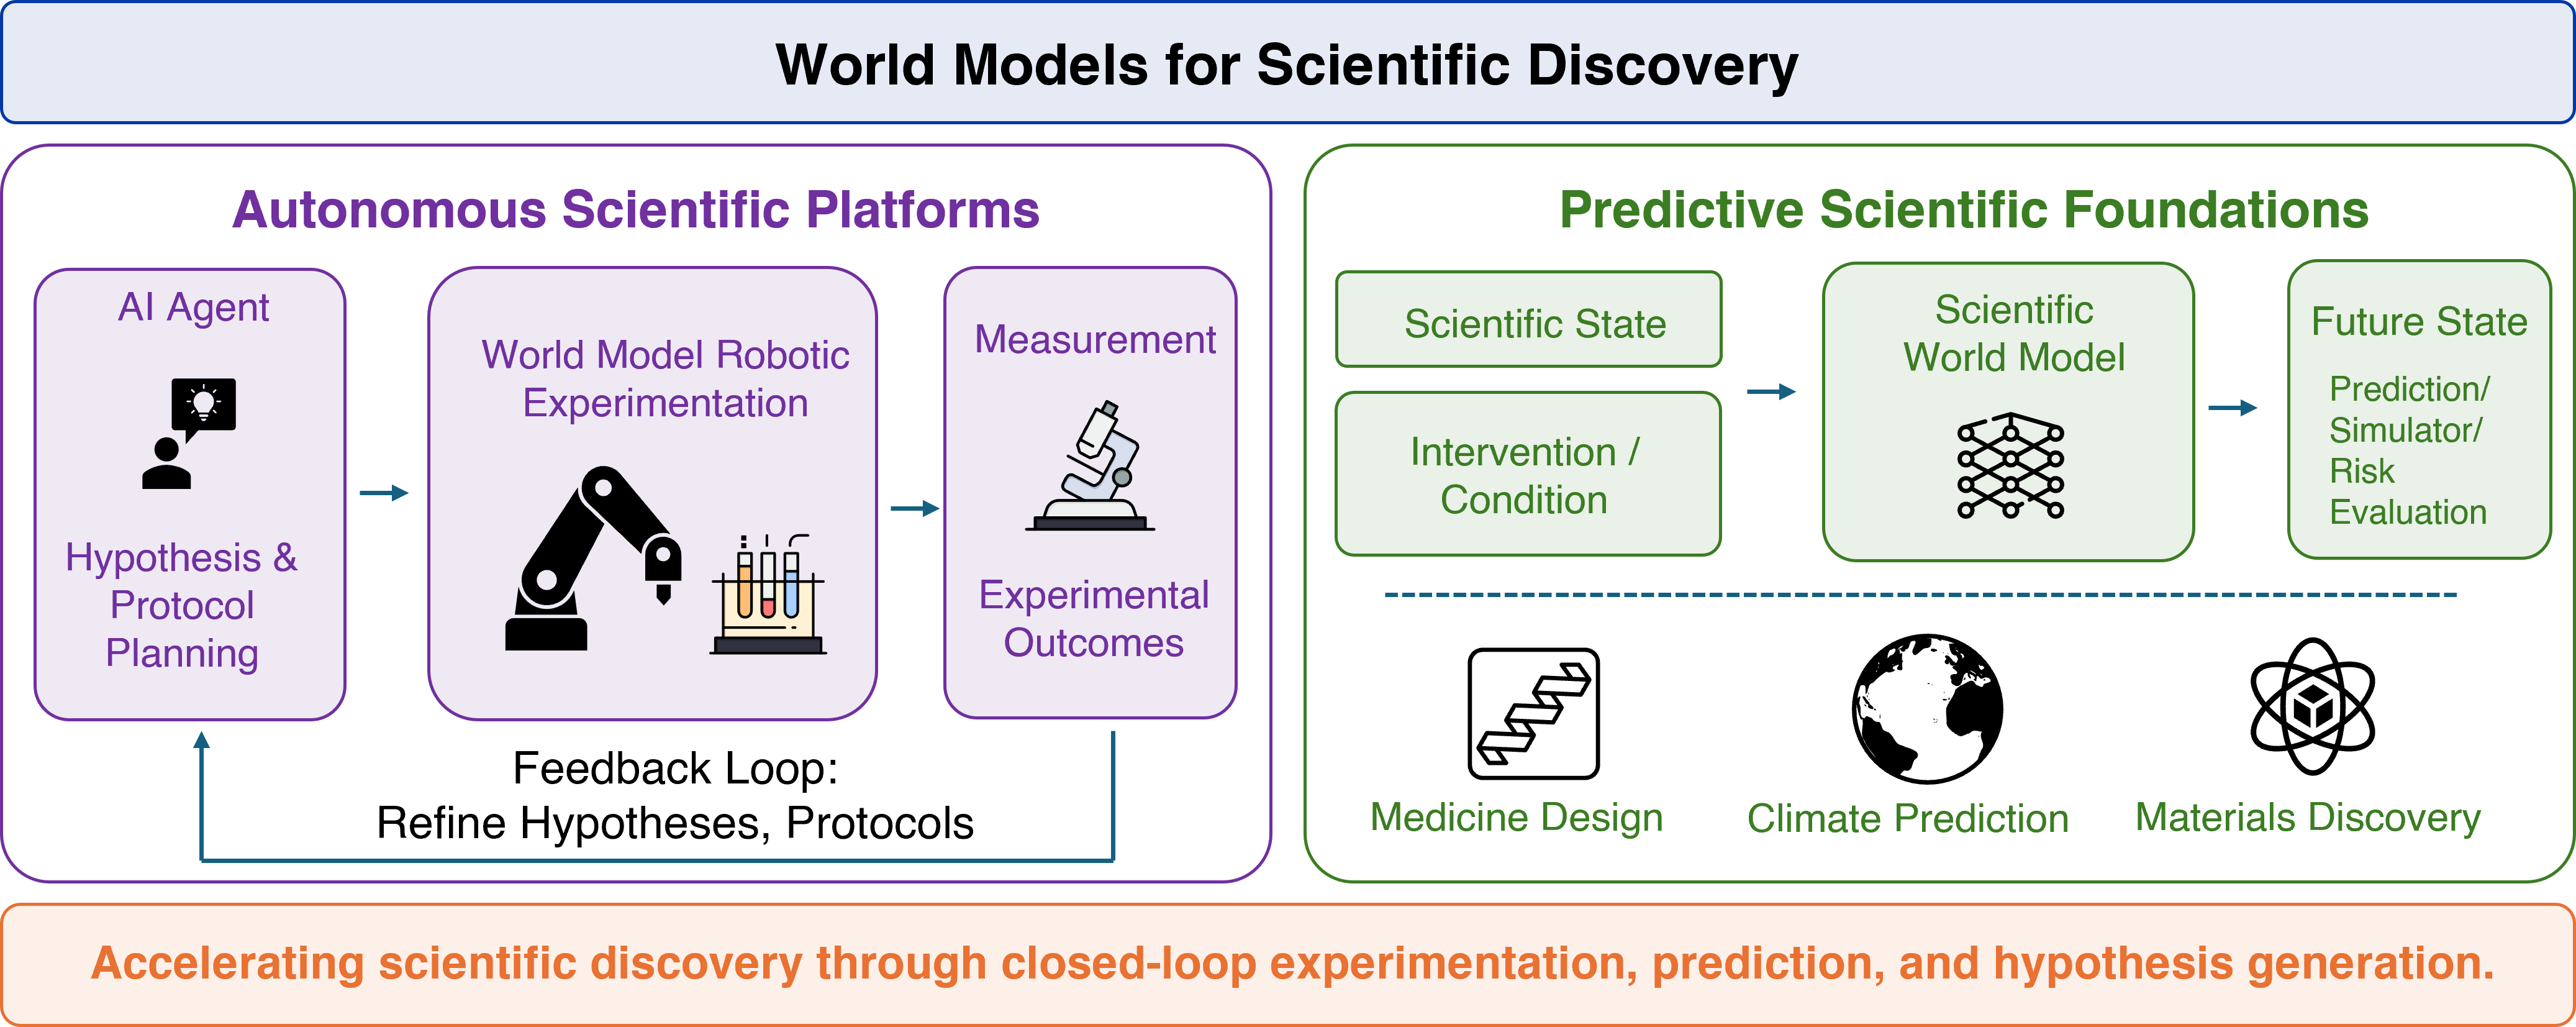
\includegraphics[width=\linewidth]{figs/science_discovery2.png}
    \caption{世界模型在科学发现中的应用。}
    \label{fig:future}
\end{figure}

世界模型已成为支撑人工智能驱动科学（AI for Science，AI4S）的基础范式，使科学发现平台能够全面进行智能化升级与优化\citep{wang2026towards}。通过提供系统性的数字框架，对客观世界的底层动力学、物理规律和运行原理建模，这些模型以两种高度互补的方式促进科学发现：赋能自主实验系统，以及充当复杂科学现象的预测基础。

首先，世界模型与人工智能智能体、机器人仪器和实验反馈结合，支持人工智能驱动的自主实验室\citep{szymanski2023autonomous,wei2025ai,wu2025ai}。它们覆盖复杂机器人操作、仪器状态动态变化等关键模态，通过协同闭环机制，与具备认知能力的大语言模型协作。真实平台部署产生的海量实验数据持续回流，用于迭代训练、改进世界模型。这形成应用驱动的双向范式：物理执行提高模型准确性，模型模拟则支持实际执行。在湿实验室中，这种整合显著提高具身系统的运行效率，使执行前的\textit{计算机内}预测推演能够预判流程与安全风险，从而减少危险，使工作流程更平顺\citep{lewis2026acht}。

其次，世界模型通过学习科学状态在不同条件或干预下如何演化，充当预测基础。它们将具身人工智能的“状态＋行动$\rightarrow$下一状态”概念扩展至科学领域，目标变为建模“科学状态＋干预／条件$\rightarrow$未来状态／响应”。科学基础模型与发现平台越来越多地支持这一角色，例如Intern-S1\citep{bai2025intern}、Intern-S1-Pro\citep{zou2026intern}和Intern-Discovery，提供推理、多模态理解、工具使用及工作流程基础设施。同时，各学科也在涌现领域专用预测世界模型。在天气与气候领域，GraphCast\citep{lam2023learning}、GenCast\citep{price2025probabilistic}、FengWu\citep{chen2023fengwu}和FengWu-W2S\citep{ling2024fengwu}等模型，将地球系统视为高维动力状态，学习其未来演化。医学与生命科学也有类似进展：Medical World Model\citep{yang2025medical}模拟以治疗为条件的肿瘤演化，Delphi-2M\citep{shmatko2025learning}则建模长期疾病进展。

最终，世界模型通过刻画超出现有人类认知边界的自然规律，推动前沿科学发现。通过符合物理规律的前向推演和反事实分析，它们识别潜在研究路径，启发新假说。这种能力不仅降低真实实验成本、加快闭环迭代，还使研究者能够探索难以直接观测的复杂过程，促进AI4S生态的长期演化与突破。

\section{开放挑战与瓶颈}
世界模型代表物理人工智能的前沿，但通往真正自主性的道路，受到感知合成与物理执行之间系统性裂缝的根本制约。当前范式能在互联网规模的被动视觉数据上轻松扩展，却在真实世界的交互性、安全关键约束面前十分脆弱。本节从整体视角分析世界模型面临的开放挑战：从使模型“视觉丰富却物理盲目”的结构性数据不对称（data asymmetry），到表面保真与可行动精度的背离，再到开环推演不断累积的漂移。我们认为，克服这些瓶颈需要根本性的范式转变：超越将世界模型仅作为生成渲染器的做法，迈向具有物理依据的模拟器和闭环交互规划器。这不仅需要考虑物理的归纳偏置与持续的环境数据采集，还需要重新构想评估框架、三方安全保证，以及能够协调集体智能与本地物理自主权的去中心化治理模式。

\subsection{数据不对称}
在渲染器、模拟器和规划器的功能分类下\citep{worldlabs2026taxonomy}，世界模型面临明确的数据不对称。渲染器可以依靠互联网规模图像、视频数据扩展，推动图像和视频生成快速进步\citep{kong2024hunyuanvideo,gao2025seedance,seedance2026seedance2,happyhorse2026}。但这些数据大多是被动、视觉性的：记录世界看起来怎样，却很少提供行动、物理属性、接触动力学或任务结果方面的监督。

相反，模拟器与规划器依赖结构更明确、可用于行动的数据。对模拟器而言，瓶颈在于可直接用于模拟的三维资产。虽然三维生成\citep{zhao2025hunyuan3d,hunyuan3d2025hunyuan3d,li2025triposg}迅速增加了视觉资产数量，但生成物体大多只适于渲染，而不能直接参与物理运行，往往缺少尺度、材料、碰撞几何、质量、摩擦、关节结构与可供性。PhysX-Anything\citep{cao2026physx}、PhysX-Omni\citep{cao2026phyomni}等近期研究，以及Lightwheel\citep{lightwheel2026}和Genesis World\citep{genesisworld2026}等工业平台，直接针对这一缺口；但真实感、非刚体动力学、长尾交互和可扩展性仍是开放挑战。对规划器而言，瓶颈进一步转向行动条件交互数据，如机器人演示、状态—行动轨迹和任务结果。Cosmos 3等近期模型\citep{nvidia2026cosmos3}将行动序列显式引入全模态世界建模，凸显行动条件数据对物理人工智能的重要性；但这类数据的可扩展性与透明程度，仍远逊于互联网视频。合成数据与模拟\citep{chang2017matterport3d,savva2019habitat,puig2024habitat,dosovitskiy2017carla,gan2020threedworld,gao2026nvidia}可部分缓解瓶颈，却引入视觉、几何、物理、行为和任务层面的分布变化。这些限制共同形成具身人工智能数据金字塔：底部是大量被动视频，中部是数量较少、可用于模拟的资产与交互轨迹，顶部则是稀缺却价值很高的触觉和力反馈。

应对这些系统性限制，需要根本改变物理智能获取世界信息的方式。现有数据采集受到规模边界与分布变化的内在限制，因此，未来世界模型的数据采集架构必须转向普遍存在、非侵入、持续运行的框架。首先，数据采集应无处不在，在不同物理场景中利用广泛、异构的采集机制，充分捕捉长尾环境。其次，数据获取流程应完全非侵入，在后台无缝运行，使采集不成为参与者的负担，也不打断日常工作；理想情况下，这种环境式采集还应通过人机协作主动提高运行效率。最后，采集必须持续进行，建立不间断的真实交互反馈循环，实时、动态、迭代地更新底层模型。

\subsection{保真度与精度}
世界模型的一项关键挑战，是感知保真度与物理精度不匹配。近期评测与研究给出了这类不匹配的经验结果。物理推理评估\citep{kang2024far,motamed2025generative,zhang2025morpheus,meng2024towards,gu2025phyworldbench,zheng2025vbench}表明，即使视觉质量提高，视频生成模型仍难以遵守物理规律和守恒约束，也难以实现分布外泛化。具身评测\citep{jiang2026robowm,shang2026worldarena}进一步揭示，视觉逼真的预测不一定转化为物理合理或可执行的机器人行为，暴露出用于操作与规划的世界模型在感知与功能之间的差距。

近期工作\citep{zhao2026phyworld,chen2026abot,wang2025physcorr,lin2026mmphysvideo}利用物理奖励、偏好配对、直接偏好优化（direct preference optimization，DPO）式训练，或结构化物理条件，在保留视觉质量的同时改善物理合理性。但当前奖励和偏好信号，仍是真实物理正确性的不完整替代，尤其难以涵盖细粒度接触、空间一致性和长尾交互。因此，感知保真度与物理精度之间的差距，仍是一项重要开放挑战。

要应对这一不匹配，需要从保真度优先的生成，转向以物理精度为中心的世界建模。首先，预训练应引入可扩展、物理信息丰富的监督，将视觉结果与潜在物理状态连接起来，如三维几何、物体运动、接触、力、材料属性和任务结果。其次，后训练应超越视觉偏好训练，引入度量约束满足、反事实有效性、长时域持续一致性和任务成功的物理奖励与评估。最后，应通过真实或高可信物理环境的闭环反馈校准世界模型，将预测与实际结果比较，并迭代改进。目标不仅是生成逼真未来，还要使世界模型预测在物理干预下能够指导行动、可以检验且可靠。

\subsection{预测误差累积}
即使世界模型局部准确，长时域部署仍可能失败，因为微小单步误差会递归反馈至后续预测。自回归推演中，每个预测观测、潜在状态或信念状态，都成为下一步上下文的一部分。因此，几何、速度、接触时刻、物体恒存性或隐藏状态估计中的细小误差会累积，将想象轨迹推离数据流形，最终偏离物理可实现行为。这一现象早已被认为是基于模型的强化学习与规划中模型偏差的主要来源\citep{talvitie2017selfcorrecting,lambert2022compounding}。视频预测与自回归视频生成也充分记录了类似失效模式：暴露偏差与时间漂移损害长时域推演\citep{nair2019hvf,chen2024diffusionforcing,huang2025selfforcing}。这同样是决策问题，而不仅是预测问题：规划器一旦开始针对不完美模型优化，就可能利用模型误差，将在真实环境中绝不可能成功的轨迹赋予高价值。在Dyna类规划中，这被强调为“幻觉出价值”\citep{jafferjee2020hallucinating}。在视觉丰富、接触密集的领域，挑战尤其突出：部分可观测性、分支未来和动力学中的剧烈不连续，使长开环推演内在脆弱。

多种缓解策略已被证明有用，但没有一种消除了问题。第一条路线是在紧凑潜在状态空间而非原始像素中预测，减少无关感知噪声，迫使模型聚焦决策相关动力学，如PlaNet和Dreamer家族\citep{hafner2019planet,hafner2019dreamer,hafner2021dreamerv2,hafner2023dreamerv3}。第二条路线通过概率动力学模型、集成和保守推演时域，使规划考虑不确定性，让行动选择更少依赖单一、脆弱的想象未来，更多依赖对可能未来经过校准的不确定性\citep{chua2018pets,janner2019mbpo,hansen2022tdmpc,hansen2023tdmpc2}。第三条路线通过自纠正目标、层级抽象和多尺度规划改善时间一致性，周期性地让长时域推理回到观测依据，而非无限期信任单一开环推演\citep{talvitie2017selfcorrecting,hafner2022director,gumbsch2024learning}。这些方法共同表明，关键目标不只是降低单步预测损失，而是让世界模型在真实规划所需时域内，保持误差有界、经过校准且适合决策。

\subsection{仿真到现实迁移}
在机器人中部署世界模型的根本挑战，是所学模拟与真实物理之间的差距。世界模型虽旨在从数据近似环境动力学，但即使微小建模误差，也可能在长时域推演中快速累积，造成不断加剧的分布变化，使真实世界预测不可靠。机器人中的这一问题尤其严重，因为接触丰富的动力学、部分可观测性及高维行动空间，使准确长期预测极其困难。

为缓解仿真到现实差距，人们探索了多种策略。经典方法是域随机化（domain randomization）：训练时让策略或动力学模型接触多样化模拟变化，促使其对视觉与物理扰动具有不变性，提高鲁棒性\citep{tobin2017domain,peng2018sim}。另一条路线关注系统辨识（system identification），从有限真实观测推断未知物理参数，用于校准模拟器或所学动力学模型\citep{nagabandi2018learning}。近期的在线适应方法，使世界模型能够利用真实反馈持续更新动力学，从而减少分布变化下的预测误差\citep{hafner2019dreamer,nagabandi2018neural}。

对基于视频的世界模型和世界行动模型（WAM）而言，这一挑战更突出：它们在高维像素空间运行，高度依赖大规模预训练所学视觉动力学先验。虽然这些模型受益于对多样互联网视频的强泛化能力，但由于物理规律、机器人本体和行动含义存在差异，将这些先验迁移至精确机器人控制仍非易事。此外，仅依靠视觉观测往往不足以支持机器人，因为视频缺少底层物理状态、本体感觉反馈及细粒度行动动力学的显式信息。加入本体感觉、触觉、力反馈及结构化机器人状态等额外模态，可为环境动力学提供互补约束，帮助缩小仿真到现实差距。应对这一差距，需要更好地整合考虑物理的归纳偏置、结构化状态表征，以及推理时自适应修正机制；这些仍是世界模型在真实机器人中规模化部署的开放挑战。

\subsection{评估与基准测试}
世界模型的评估格局仍很分散。世界模型跨越视觉预测、物理模拟、行动规划和下游决策，不同研究群体常使用不同指标与评测。对预测及生成模型，常用指标包括均方误差（mean squared error，MSE）等配对重建误差，以及FID、FVD等分布或感知指标，度量生成图像、视频相对于真实数据的质量。对控制与规划任务，通常依据任务表现评估，如奖励、回合回报、成功率或任务完成情况。泛化通常在分布外（OOD）或零样本条件下评估，在未见环境、物体、任务或动力学上度量相同预测或任务指标。在机器人和自动驾驶等安全关键场景，不确定性校准等面向可靠性的指标同样重要，因为智能体必须知道何时预测或计划不可靠，才能安全推演轨迹并进行考虑风险的规划。

在评测层面，这些指标用于一系列代表性基准测试。对预测式与生成式视频模型，VBench\citep{huang2023vbench}和VBench-2.0\citep{zheng2025vbench}等套件评估视频质量、时间一致性、与提示的符合程度及内在忠实性；与Cosmos 3一同引入的Cosmos-HUE等人工评估规程\citep{nvidia2025cosmos}，评估生成式与全模态世界模型的输出。对三维／四维世界生成，WorldScore\citep{duan2025worldscore}和4DWorldBench\citep{lu20264dworldbench}将评估从二维视频质量扩展到可控性、动力学和时空一致性。对物理一致性及世界模拟器保真度，PhyGenBench\citep{meng2024towards}、WorldModelBench\citep{li2026worldmodelbench}和PhyWorldBench\citep{gu2025phyworldbench}等面向物理的评测，考察生成视频是否遵循物理常识、具有物理真实感；WorldSimBench\citep{qin2024worldsimbench}进一步从感知和行动两个层面，将视频生成模型作为世界模拟器评估。

对行动条件与下游功能评估，Atari／ALE\citep{bellemare2013arcade}和DM Control\citep{tassa2018deepmind}常用于基于模型的强化学习和连续控制；Habitat\citep{savva2019habitat}和CARLA\citep{dosovitskiy2017carla}在模拟中评估具身导航和自动驾驶；RoboArena\citep{atreya2025roboarena}将评估扩展到真实机器人策略；EWMBench\citep{yue2025ewmbench}从场景一致性、运动正确性与语义符合程度评估具身世界模型；WorldArena\citep{shang2026worldarena}评估其功能效用。对于交互式世界模型，WBench\citep{ying2026wbench}和WorldMark\citep{xu2026worldmark}等近期评测，考察模型能否遵循多轮交互、保持控制一致性和物理合理性。作为补充，MBench\citep{zhang2026mbench}、WorldPrediction\citep{chen2025worldprediction}和WorldReasonBench\citep{wu2026worldreasonbench}等长时域状态推理评测，考察世界模型能否维持持续状态、支持程序性规划，并生成在物理、社会、逻辑与信息层面具有一致状态演化的未来视频。

近期CoW-Bench进一步围绕“一致性三位一体”——模态、空间与时间一致性——组织世界模型评估，测试生成模型在复杂多模态情境下，能否保留跨模态对应关系、具有三维感知的空间结构、物体恒存性，以及物理合理的时间演化\citep{wei2026trinityconsistencydefiningprinciple}。尤其需要指出，现有评测往往忽略推理效率；但真实物理交互所需的闭环控制频率，无法容忍高延迟推演。亚秒级生成速度不只是计算指标，也是基本安全要求，因为推理滞后会直接引发高动态环境中的控制不稳定。

归根结底，当前评估范式的根本瓶颈，是缺少真实物理依据。虚拟模拟器采用简化物理引擎，使世界模型能够利用在现实中失效的非因果捷径。真正的验证需要真实部署和持续物理交互，以面对未被建模的随机动力学。然而，转向物理平台也引入了真实性与实验控制程度之间的重要取舍。核心开放挑战是评测标准化与公平性。与可复现的软件容器不同，物理评估受到硬件退化、初始状态不一致，以及极高重复成本的影响。如何制定规程，规范不同机器人本体的评估，并将硬件噪声与模型能力分离，仍是下一步的重要研究方向。

\subsection{安全、透明性与可持续性}
\paragraph{安全探索与三方交互安全。}
具身人工智能和自主智能体的部署引入显著物理风险，因为在不受约束的环境中实时决策，比孤立的数据分析危险得多。模拟与现实的残余差距永远无法彻底消除，因此，未经测试就在真实环境探索，本身便具有危险\citep{billard2025roadmap}。物理世界模型充当学习得到的内部模拟器，使智能体策略能在部署前通过想象推演充分优化，从而缓解风险。推理时，这些模型提供连续状态表征与多步规划，以预判行动后果。与重型或高吞吐量机械交互时，为保证安全，必须在推演引擎中嵌入约束方法和严格的不确定性阈值；一旦预测外推至不安全状态区域，就停止执行。由于环境、机器人本体和任务会在智能体运行生命周期中演化，安全探索必须是一项与终身学习耦合的持续能力。

此外，这种安全范式会在动态三方生态中非线性扩展，涉及人机协调、环境反馈的共同演化，以及异构多智能体同步。首先在人机交互中，安全不止于反应式避障，而成为博弈论意义上的认知协调；人类应对行为会根据机器人轨迹动态变化，因此世界模型必须将心智理论框架融入潜在推演，主动适应隐含人类意图。其次，在机器—环境循环中，世界模型必须体现因果双向性：不仅预测智能体如何改变周围环境，还要预测非平稳环境反馈，如结构疲劳或热变形，如何反过来破坏控制保证。第三，不同形态的异构智能体共处时，主要风险会从单个控制器失效，转向系统性共振：各自世界模型之间不对称的不一致，可能级联成分布式碰撞。

\paragraph{透明性、可解释性与可验证控制。}
要合乎伦理、可靠地部署世界模型，可解释性对建立操作人员信任和厘清责任至关重要。与传统黑箱端到端策略相比，世界模型依赖环境动力学的显式表征，因而提供了结构更明确的透明化路径。但深度神经网络本身难以解释，将这些动力学转化为可验证预测，仍是开放工程问题。仅依赖人为构建的可解释层，维持含义清晰的潜在维度，以运行时验证速度界限、能量守恒等不变量，还不够。所学组件必须系统地结合控制理论或形式化验证框架，取得可证明的稳定性与约束满足，使预测具有数学保证，而非不受约束的外推。

此外，操作人员进入循环后，单靠技术可解释性无法消除系统风险。世界模型高度逼真的模拟输出，可能引发自动化偏差（automation bias）等认知弱点；已有研究记录，操作人员容易过度依赖看似权威的模型预测，即使这些预测错误或处在分布外\citep{parasuraman1997humans}。这一弱点源于人如何在认知上接受解释，而非底层模型准确性，因此仅改善可解释性无法解决。缓解自动化偏差，需要面向用户的界面显式呈现认识不确定性，例如标记偏离已验证训练分布的推演，使人的信任准确对应系统的客观可靠程度。

\paragraph{合乎伦理的部署与保护隐私的治理。}
合乎伦理的部署是一项独立要求，涉及根据世界模型的人类相关预测与数据采取行动是否合法正当。这带来三项中心义务。第一，预测人类行为以规划机器人行动时，世界模型不得依赖基于偏见的画像\citep{billard2025roadmap}。这一约束极难落实，因为预测直接进入物理行动，而非供人拒绝的信息建议。第二，数据采集存在严格隐私边界：物理交互数据集中的参与者必须不可识别，不应能推断敏感属性，记录也不得超出原始范围转作他用\citep{billard2025roadmap}。这些约束虽必要，却严重限制大规模人类交互数据集的构建。第三，透明性是事故责任认定的前提，但商业上普遍采用闭源感知和控制系统，抵制独立审查，这与透明要求直接冲突\citep{billard2025roadmap}，使问责仍是开放治理挑战。

为解决跨机构数据汇集障碍并兼顾商业保密，协作框架必须转向联邦世界模型（federated world model）。在这一范式下，本地数据孤岛保持原状，参与方只交换潜在梯度或网络权重。为防御梯度反演攻击（gradient inversion attack），这些架构必须整合安全多方计算（secure multi-party computation），或使用硬件强制保护的可信执行环境（trusted execution environment，TEE）进行加密联合训练。关键在于，为适应不同机构环境中的非独立同分布（Non-IID）数据\footnote{译注：原文将Non-IID展开为“non-identical and independently distributed”，与该缩写通常表示的“非独立同分布”不符；此处按Non-IID及上下文翻译。}，框架必须将不变的物理常识——全局学习、普遍共享，以支撑集体智能——与变化很大的领域特定潜在表征——本地保留——分离，从而兼顾集体智能与本地数据主权。

不过，还有一项重要限制：当前优化几乎只关注训练和推理运行阶段的能耗，完全忽略硬件整个生命周期的环境足迹。完整的可持续性评估必须纳入生命周期管理框架，涵盖材料开采、制造与报废处理\citep{billard2025designing}。稀土采矿、软执行器聚合物合成和半导体制造等上游环境成本，在当今人工智能评测中大多被忽略。可持续计算文献表明，隐含碳排放（embodied carbon）与运行碳排放（operational carbon）往往存在取舍；孤立优化其中一项，可能无意中放大另一项\citep{lee2025view}。因此，仅依据计算指标提出效率结论，从根本上说是不完整的，必须审慎解读。

\section{发展路线图}\label{sec:roadmap}
\begin{figure}[t]
    \centering
    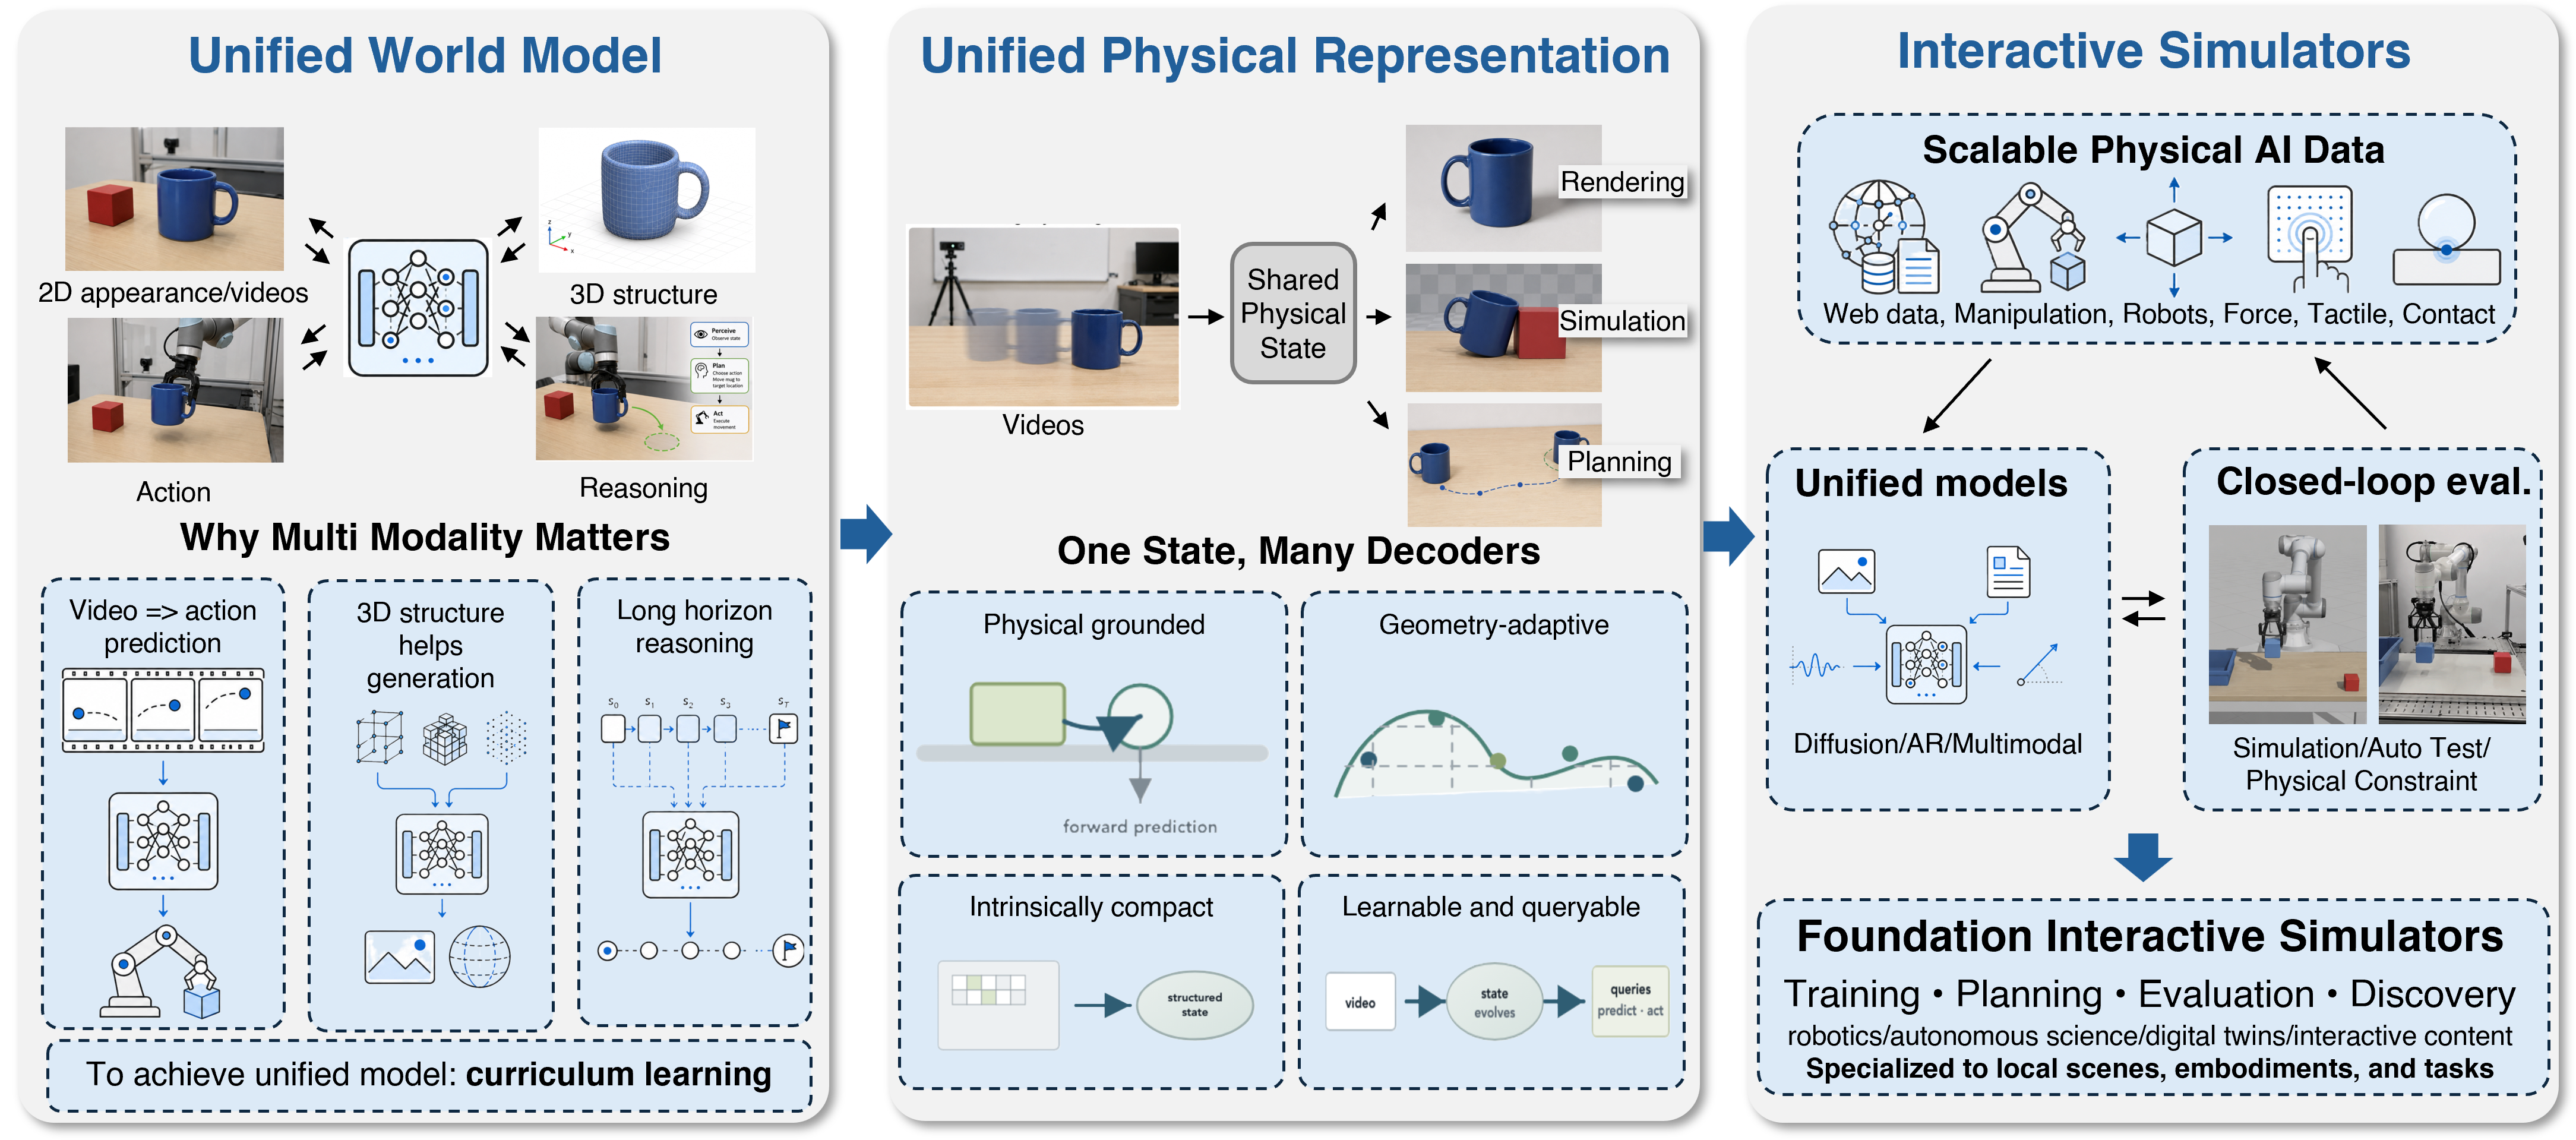
\includegraphics[width=\linewidth]{figs/future2.png}
    \caption{发展下一代世界模型的分阶段路线图。}
    \label{fig:roadmap}
\end{figure}

基于前述讨论，构建未来鲁棒的物理世界模型，需要经过图\ref{fig:roadmap}所示的三个递进阶段。首先，世界模型必须利用多种统一模态，整合各类异步采样信号，使模型能够在大多数物理环境中工作。其次，必须将这些不同模态提炼为统一物理表征（Unified Physical Representation），即单一、高度压缩的内部状态；各种下游任务都能直接从这一状态解码出渲染、模拟与规划。第三，结合先进架构与具有物理依据的数据，扩展这些表征，进而实现基础模型规模的交互模拟器（Foundation-Scale Interactive Simulator）。在这一最终阶段，世界模型成为闭环、可复用环境，允许智能体在真实执行之前安全地探索、评估和改进行动。

\subsection{迈向统一多模态世界模型}
统一多模态是未来世界模型的中心问题，因为准确预测要求共同表示外观、空间结构、状态、行动和长时域推理。视频捕捉运动，三维结构支持视角一致的记忆，行动—状态信号解释可控变化，语义推理把局部预测与长期目标联系起来。因此，统一世界模型不应只是合并模态，还应将这些信号与世界变化方式关联起来。统一多模态对这一问题至关重要，原因有以下几点。

第一，长时域推理需要多模态信息。虽然视频扩散模型能生成可信未来，但操作等许多任务需要长期未来规划，单纯视频扩散模型在有限计算资源下可能难以实现。因此，模型需要搜索、策略或价值信号，在生成分支之间选择。基于扩散的控制系统常将生成与树搜索或行动策略配对\citep{huang2025forgetree,chi2023diffusionpolicy}。引入更多模态后，模型在长期感知、预测与行动选择方面具有更大扩展潜力。

第二，三维等模态能够提供有益补充，在数据稀缺时改善泛化。机器人与驾驶数据集很少覆盖智能体可能遇到的所有相机视角、物体姿态或空间配置。稀疏视角重建与具有几何依据的视频生成，可以合成缺失视角、姿态，以及运动一致的样本，用于训练或测试可控模型\citep{yu2020pixelnerf,liu2023zero123,kang2026geonvs}。这使多模态成为改善泛化的实际途径，因为没有任何单一模态能够充分覆盖罕见空间情况。

第三，行动与状态信号将视频预测从被动预报转化为具身预测。仅凭视觉观测，不能确定哪种抓取会成功，因为同一场景在推、抓取或不行动后，可能产生不同未来。近期视频—行动世界模型，将视觉上下文与显式行动和状态输入结合\citep{zhou2026tau0wm,alradi2026aeroworld}。这说明，仅有视觉规模还不够；模型还必须编码使变化可控的变量。

实际可行的路径，是将统一视为课程（curriculum），而非单一混合词元流。训练可以从静态表征学习开始，用JEPA等图像目标建立语义特征\citep{assran2023ijepa}；随后加入视频、状态、行动和具身数据，同时用紧凑潜在行动，将可控变化与背景外观分离\citep{bruce2024genie,bi2025motus}。

\subsection{迈向统一物理表征}
如前所述，信息压缩是实现统一世界模型的关键。为了将高维感官观测压缩为保留物理世界结构的共享内部状态，表征选择比任何单个渲染器、模拟器或规划器的选择都更重要。然而，当前多数系统维持三种彼此分离的世界定义：渲染采用辐射场或高斯基元等以外观为中心的基元\citep{mildenhall2020nerf,kerbl20233dgaussians}；模拟采用网格或粒子；规划采用占据栅格（occupancy grid）或物体槽位。它们之间的转换有损且缺乏统一原则。因此，必须同时支持感知、模拟与控制的世界模型，会提出这些解码器尚未回答的前置问题：三者究竟可以从哪一种单一内部状态解码出来？

最有希望的长期方向，不是孤立地改进渲染器、模拟器或规划器，而是建立一种\emph{共享物理表征}，使每种功能都成为对它的解码操作。这一表征应具有以下性质。首先，它应有物理依据、可用于模拟，使同一状态承载前向预测所需的动力学与接触结构，而不只是表面外观。其次，它应适应几何差异，容纳真实场景中异构、不规则的几何，而不强加规则栅格或固定模板。此外，它应内在紧凑，编码结构化状态而非稠密场，使容量用于缓慢变化、与决策相关的物理因素，而非像素级细节。在这种表征下，几何、运动、材料属性、外观、语义身份、不确定性与交互状态，将共同编码于一个持续保持的状态中；渲染、模拟与规划不再需要三种独立世界定义，而成为对同一压缩物理状态的不同解码操作：解码为像素或泼溅基元以渲染，解码为形变、应力与接触变量以模拟，或解码为“物体—部件—可供性”结构以规划行动。

这种“一个状态，多个解码器”原则已有部分先例。例如，PhysGaussian\citep{xie2024physgaussian}从同一组高斯核驱动物理模拟与渲染。更广泛的挑战，是设计同时满足各项要求的统一表征：1）能够解码外观、有模拟依据、适应不同几何且紧凑；2）能够从互联网规模视觉数据学习，并将这些数据压缩为持续保持的物理状态；3）该状态能够通过解析或所学动力学演化，并通过任务专用查询接口提供感知预测、反事实模拟与控制。具体采用何种基础结构，仍是开放问题。归根结底，通往物理世界模型的中心问题是：\textit{怎样一种紧凑内部结构，能够保留足够的物理与语义信息，以支持具身智能的所有下游投影？}

\subsection{基础模型规模的交互模拟器}
最后，世界模型的另一用途，是构建支持行动想象、任务生成、反馈整合或持续改进的交互模拟器。世界模型有助于扩大模拟器规模，提供可复用环境，使智能体与科学系统能够在真实实验之前测试行动、评估风险并探索可能结果。

这一愿景受到大语言模型和近期视频生成模型规模扩展成功的启发：更大模型、更广泛数据与更多计算，带来了推理和泛化能力的系统性提升。这给世界模型提出中心问题：物理动力学能否出现类似尺度行为？更具体地说，更大的模型、更多样的数据、可扩展的交互训练数据集，以及物理信息丰富的标注，能否提高世界模型维持物理一致性、预测长时域动力学、可靠响应智能体行动并充当交互模拟器的能力？

为实现这一目标，需要考虑三个关键方面。首先，需要可扩展模型架构，同时支持高保真世界预测与可靠的行动条件交互。近期扩散和流匹配模型能够生成高质量视觉未来，自回归及大语言模型式架构在长上下文序列建模和推理方面具有优势。Cosmos 3等较新的统一多模态模型，以及Bernini等规划器—渲染器框架进一步表明，语言、视觉、视频、音频和行动可以在更加统一的建模框架中被处理或协调。对基础模型规模交互模拟器而言，关键架构问题仍然开放：什么样的模型设计，能够在引入力、触觉反馈、接触状态及本体感觉等更丰富物理模态的同时，扩展可控交互能力？

其次，基础模型规模交互模拟器的发展，既依赖互联网视频，也依赖可扩展物理数据集的构建。互联网视频引入通用视觉与行动先验；第一人称操作视频以行动或手部运动标注补充；真实机器人轨迹提供具有物理依据的控制信号。除这些来源外，更丰富的物理监督同样重要，包括三维状态、物体运动、接触事件、力、触觉反馈、热信号和材料属性。

第三，物理交互模拟器必须在闭环场景中检验。学习得到的模拟器可以为策略训练与评估提供低成本交互环境，但其自身预测仍须根据真实结果或可靠物理约束验证。因此，未来系统需要超越视觉可信性的评估规程，度量预测未来是否与行动保持因果一致，能否在长时域保持一致，以及能否预测机器人或人工智能驱动自主湿实验室中的真实执行结果。

\section{展望：通往物理通用人工智能之路}
\label{sec:path-to-physical-agi}
大语言模型（LLM）使机器以前所未有的程度掌握了人类语法、语义和积累的知识。然而，尽管大语言模型对我们如何描述现实有百科全书般的理解，它们却缺乏对物理现实本身的根本依托。我们正在迅速接近离身智能的极限\citep{coveney2025wall}。

语言模型与世界模型的关系，定义了人工智能发展的下一次重大范式转变。要勾勒通往通用人工智能（artificial general intelligence，AGI）的更广阔道路，必须认识到人工认知的一个基本事实：i）语言赋予机器谈论世界的方式；ii）世界模型将使机器理解世界、想象世界、借助世界进行推理，并在其中行动。如果AGI需要在物理领域导航和操作，就不能只靠预测序列中的下一个词完成这些任务。它必须原生地具备对物理、因果、空间推理和时间的直觉理解，必须能够在行动前模拟后果——预测现实本身的下一个状态；更重要的是，它需要评估给定当前物理智能体，在真实世界中哪些任务可能实现。

\paragraph{三位一体架构：自主演化的引擎}
要实现物理通用人工智能（Physical AGI）愿景，仅有基于历史数据被动训练的静态模型还不够。AGI需要一个动态、自我演化的系统，能够持续与真实世界交互并自主学习。为此，我们提出\textbf{三位一体架构（Trinity Architecture）}这一概念：一个三部分的认知循环，旨在自主弥合数字推理与物理能力之间的差距。架构由三个相互依赖的组件构成：
\begin{itemize}
\item \textbf{智能体（Agent）：任务执行引擎。}行动者（Actor）即物理智能体，接收任务指令，并以物理方式（或物理模拟方式）尝试完成任务。它将高层意图转化为环境中细粒度、序贯的行动。
\item \textbf{评估器（Evaluator）：任务完成的裁判。}智能体运行时，评估器观察轨迹数据，评价任务完成的有效性与效率，对失败、物理规律违反或次优运动提供精确反馈。
\item \textbf{世界模型：核心模拟器与课程设计者。}世界模型接收智能体生成、经评估器评分的轨迹数据，通过观察交互，学习世界的底层物理、动力学和因果关系。关键在于，世界模型理解智能体当前能力的确切\emph{边界}，利用内部模拟，想象并提出复杂程度逐渐提高、\textit{略超出}智能体当前能力的新任务，充当自动课程生成器。
\end{itemize}

这里，世界模型承担关键角色：i）内化世界知识；ii）了解当前行动者可行任务的边界；iii）通过提出新任务，指导下一轮智能体—世界交互。这也类似于人类学习和使用脑内世界模型的方式\citep{taniguchi2023world,deng2025simura}。行动者与评论家组件同样可以借助大语言模型增强，例如实现为基于大语言模型的多智能体系统\citep{yang2025unlocking}；因此，这些组件中的规划、推理与决策，自然依赖大语言模型的认知智能。由此，三位一体架构提供了大语言模型与世界模型相互增强的机制。

\begin{figure}
    \centering
    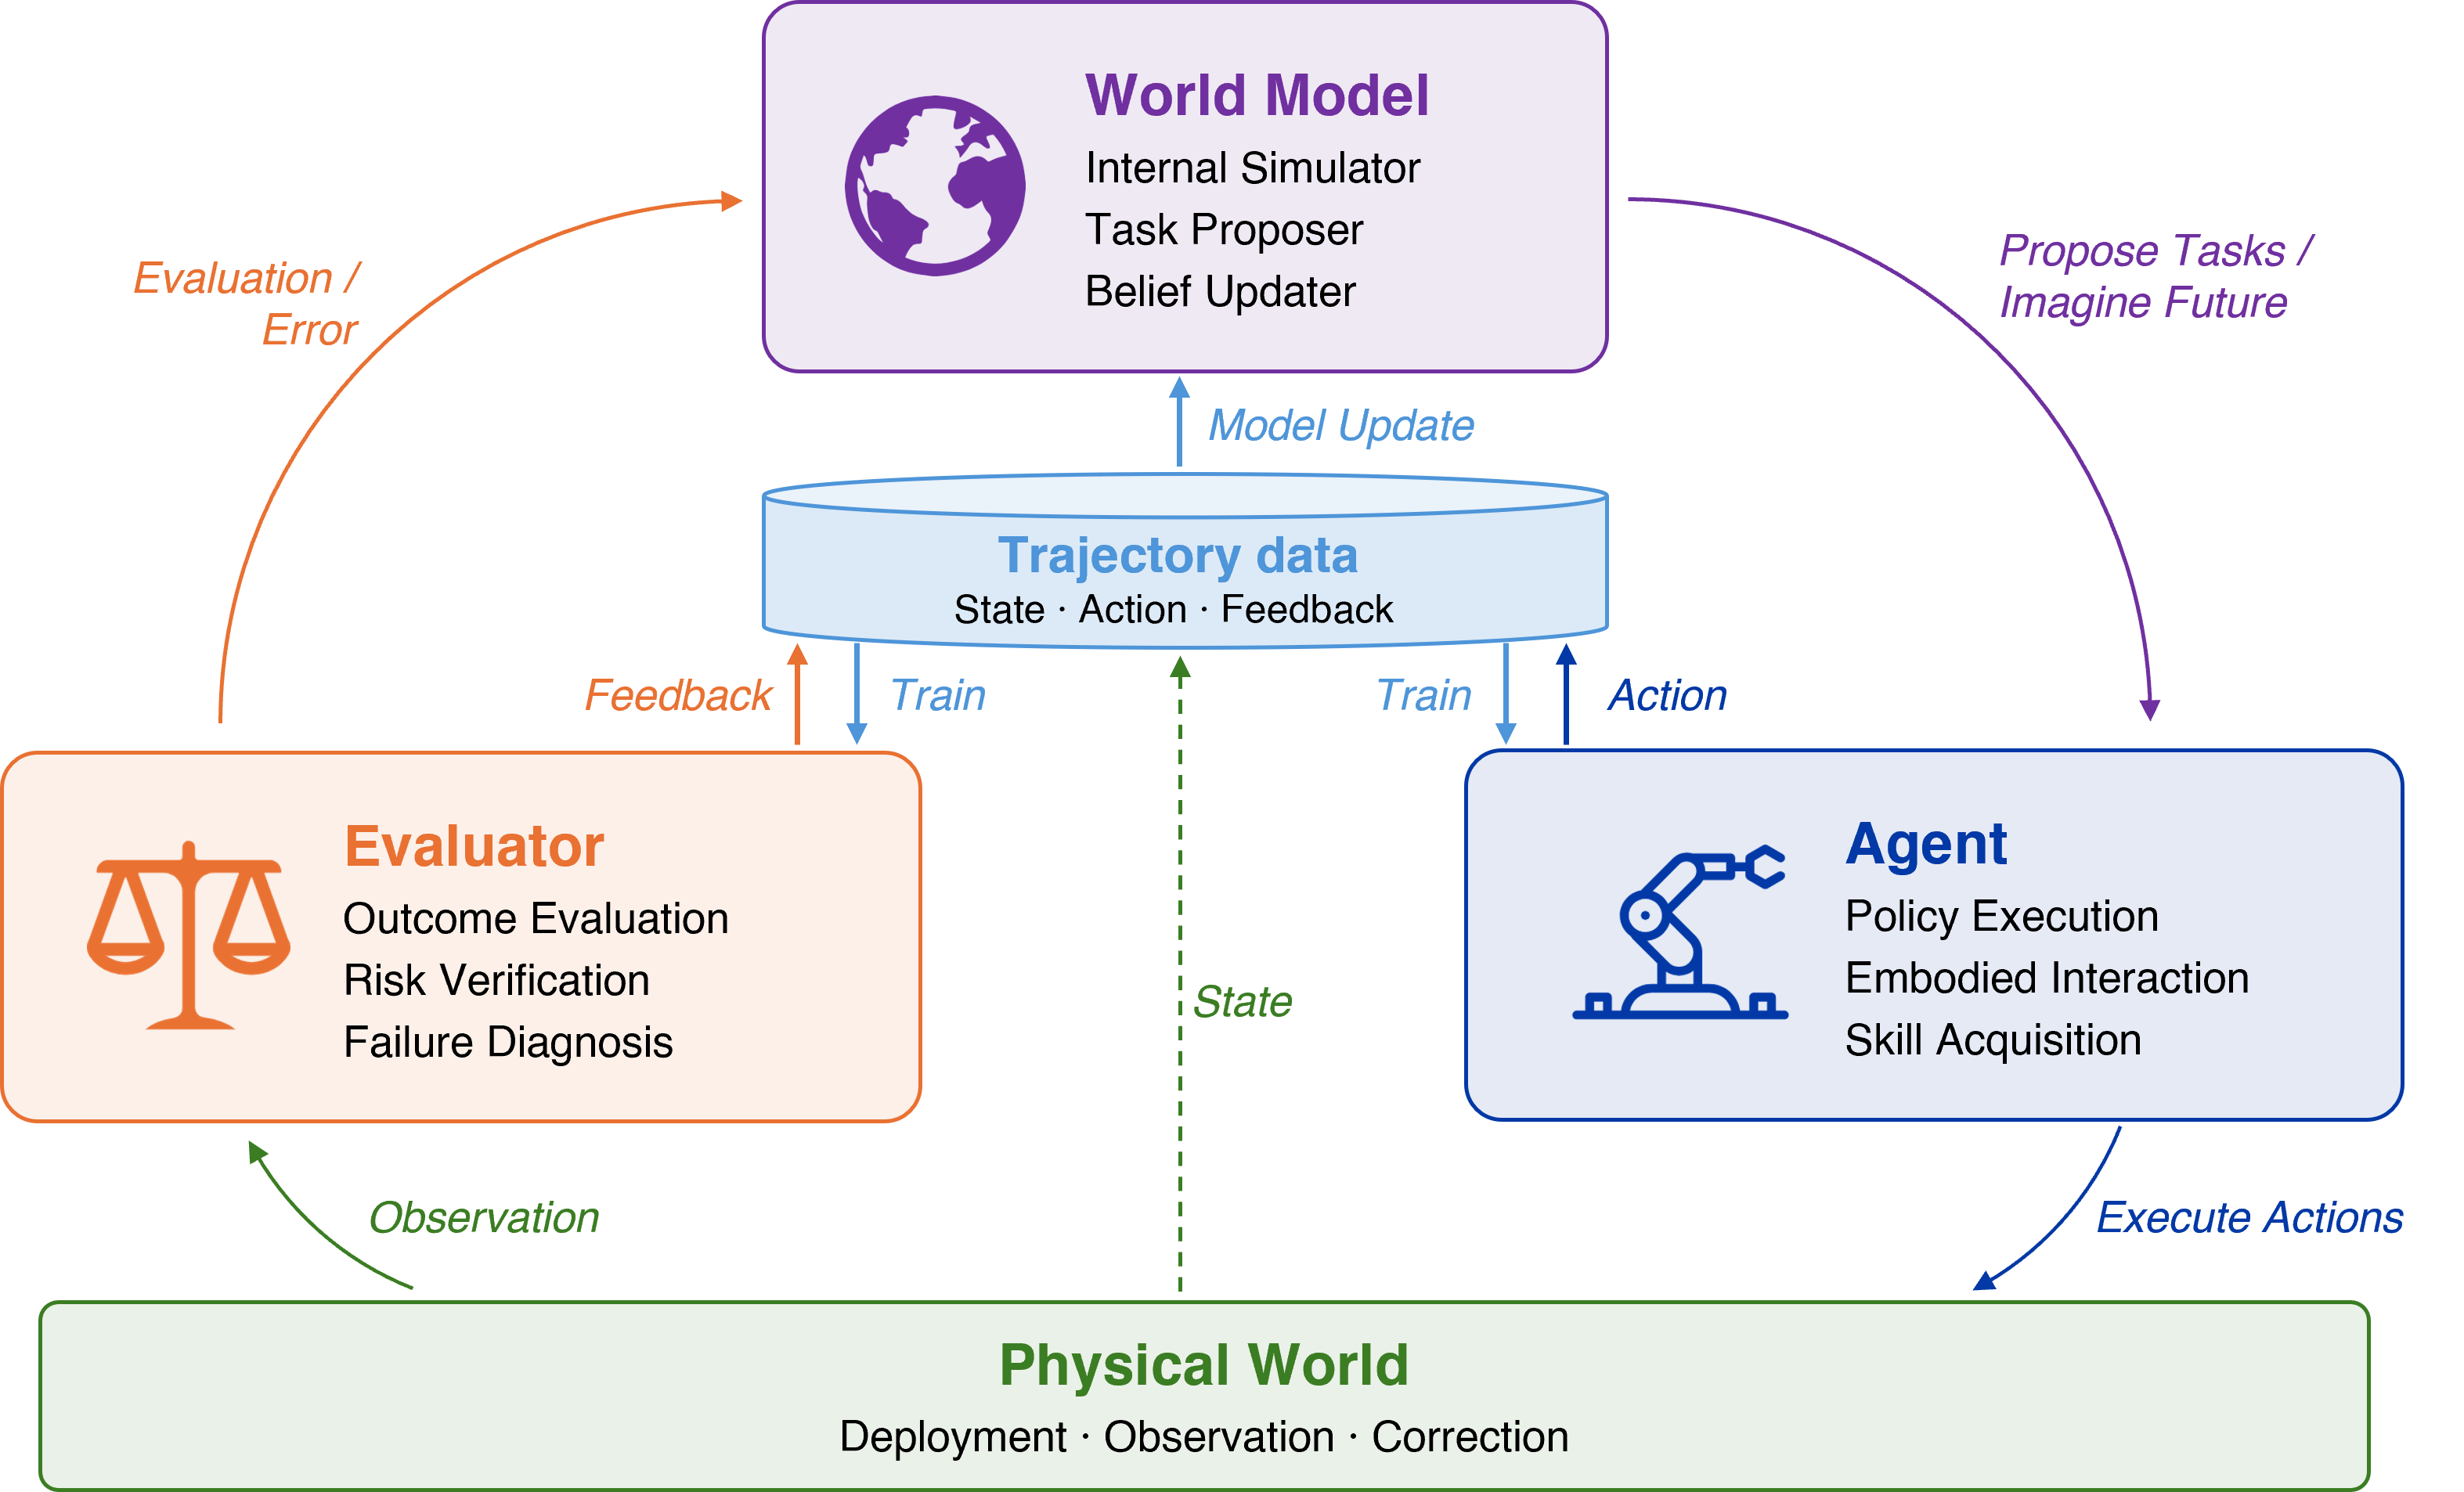
\includegraphics[width=0.85\linewidth]{figs/trinity_architecture2.png}
    \caption{三位一体架构概览。}
    \label{fig:trinity}
\end{figure}

\paragraph{通过与世界交互迈向AGI}
这一三位一体体系的真正力量，在于与现实持续交互。循环同时运行于数字模拟与物理世界。世界模型可以安全地想象数千种情境，并提出任务，让行动者先在高保真数字孪生（digital twin）中尝试。行动者掌握这些任务后，系统将所学直觉部署到物理世界，评论家评估现实中不可避免的摩擦与噪声，再将新数据反馈给世界模型。

通过不断行动、评估和更新内部模拟的循环，人工智能不再完全依赖人工整理的数据集，而开始像生物智能一样，通过物理试验、错误和想象来学习。这一三位一体架构不仅是改进机器人的蓝图，也是将人工智能从被动对话者转变为主动的物理AGI的演化引擎。


\section*{贡献者}
本文贡献者如下，按姓氏的字母顺序排列：
Xinyuan Chen, Haoyu Guo, Shi Guo, Bingqi Jiang, Chunhua Shen, Xing Shen, Tianfan Xue, Yufei Xue, Mulin Yu, Weinan Zhang, Bin Zhao, Bowen Zhou, Ming Zhou.



\bibliographystyle{plainnat}
\bibliography{wm-pjlab}
\end{document}
